%&preformat-synopsis
\RequirePackage[l2tabu,orthodox]{nag} % Раскомментировав, можно в логе получать рекомендации относительно правильного использования пакетов и предупреждения об устаревших и нерекомендуемых пакетах

% Откомментируйте, чтобы отключить генерацию закладок в pdf
% \PassOptionsToPackage{bookmarks=false}{hyperref}
\documentclass[a5paper,10pt,twoside,openany,article]{memoir} %,draft

%%%%%%%%%%%%%%%%%%%%%%%%%%%%%%%%%%%%%%%%%%%%%%%%%%%%%%%%%%%%%%%%%%%%%%%%%%%%%%%%
%%%% Файл упрощённых настроек шаблона, общих для диссертации и автореферата %%%%
%%%%%%%%%%%%%%%%%%%%%%%%%%%%%%%%%%%%%%%%%%%%%%%%%%%%%%%%%%%%%%%%%%%%%%%%%%%%%%%%

%%% Режим черновика %%%
\makeatletter
\@ifundefined{c@draft}{
  \newcounter{draft}
  \setcounter{draft}{1}  % 0 --- чистовик (максимальное соблюдение ГОСТ)
                         % 1 --- черновик (отклонения от ГОСТ, но быстрая
                         %       сборка итоговых PDF)
}{}
\makeatother

%%% Пометки в тексте %%%
\makeatletter
\@ifundefined{c@showmarkup}{
  \newcounter{showmarkup}
  \setcounter{showmarkup}{0}  % 0 --- скрыть пометки
                              % 1 --- показывать пометки
}{}
\makeatother

%%% Использование в pdflatex шрифтов не по-умолчанию %%%
\makeatletter
\@ifundefined{c@usealtfont}{
  \newcounter{usealtfont}
  \setcounter{usealtfont}{1}    % 0 --- шрифты на базе Computer Modern
                                % 1 --- использовать пакет pscyr, при его
                                %       наличии
                                % 2 --- использовать пакет XCharter, при наличии
                                %       подходящей версии
}{}
\makeatother

%%% Использование в xelatex и lualatex семейств шрифтов %%%
\makeatletter
\@ifundefined{c@fontfamily}{
  \newcounter{fontfamily}
  \setcounter{fontfamily}{1}  % 0 --- CMU семейство. Используется как fallback;
                              % 1 --- Шрифты от MS (Times New Roman и компания)
                              % 2 --- Семейство Liberation
}{}
\makeatother

%%% Библиография %%%
\makeatletter
\@ifundefined{c@bibliosel}{
  \newcounter{bibliosel}
  \setcounter{bibliosel}{1}   % 0 --- встроенная реализация с загрузкой файла
                              %       через движок bibtex8;
                              % 1 --- реализация пакетом biblatex через движок
                              %       biber
}{}
\makeatother

%%% Вывод типов ссылок в библиографии %%%
\makeatletter
\@ifundefined{c@mediadisplay}{
  \newcounter{mediadisplay}
  \setcounter{mediadisplay}{1}   % 0 --- не делать ничего; надписи [Текст] и
                                 %       [Эл. ресурс] будут выводиться только в ссылках с
                                 %       заполненным полем `media`;
                                 % 1 --- автоматически добавлять надпись [Текст] к ссылкам с
                                 %       незаполненным полем `media`; таким образом, у всех
                                 %       источников будет указан тип, что соответствует
                                 %       требованиям ГОСТ
                                 % 2 --- автоматически удалять надписи [Текст], [Эл. Ресурс] и др.;
                                 %       не соответствует ГОСТ
                                 % 3 --- автоматически удалять надпись [Текст];
                                 %       не соответствует ГОСТ
                                 % 4 --- автоматически удалять надпись [Эл. Ресурс];
                                 %       не соответствует ГОСТ
}{}
\makeatother

%%% Предкомпиляция tikz рисунков для ускорения работы %%%
\makeatletter
\@ifundefined{c@imgprecompile}{
  \newcounter{imgprecompile}
  \setcounter{imgprecompile}{0}   % 0 --- без предкомпиляции;
                                  % 1 --- пользоваться предварительно
                                  %       скомпилированными pdf вместо генерации
                                  %       заново из tikz
}{}
\makeatother
          % общие настройки шаблона
%%% Проверка используемого TeX-движка %%%
\newif\ifxetexorluatex   % определяем новый условный оператор (http://tex.stackexchange.com/a/47579)
\ifxetex
    \xetexorluatextrue
\else
    \ifluatex
        \xetexorluatextrue
    \else
        \xetexorluatexfalse
    \fi
\fi

\newif\ifsynopsis           % Условие, проверяющее, что документ --- автореферат

\usepackage{etoolbox}[2015/08/02]   % Для продвинутой проверки разных условий
\providebool{presentation}

\usepackage{comment}    % Позволяет убирать блоки текста (добавляет
                        % окружение comment и команду \excludecomment)

%%% Поля и разметка страницы %%%
\usepackage{pdflscape}  % Для включения альбомных страниц
\usepackage{geometry}   % Для последующего задания полей

%%% Математические пакеты %%%
\usepackage{amsthm,amsmath,amscd}   % Математические дополнения от AMS
\usepackage{amsfonts,amssymb}       % Математические дополнения от AMS
\usepackage{mathtools}              % Добавляет окружение multlined
\usepackage{xfrac}                  % Красивые дроби
\usepackage[
    locale = DE,
    list-separator       = {;\,},
    list-final-separator = {;\,},
    list-pair-separator  = {;\,},
    list-units           = single,
    range-units          = single,
    range-phrase={\text{\ensuremath{-}}},
    % quotient-mode        = fraction, % красивые дроби могут не соответствовать ГОСТ
    fraction-function    = \sfrac,
    separate-uncertainty,
    ]{siunitx}[=v2]                 % Размерности SI
\sisetup{inter-unit-product = \ensuremath{{}\cdot{}}}

% Кириллица в нумерации subequations
% Для правильной работы требуется выполнение сразу после загрузки пакетов
\patchcmd{\subequations}{\def\theequation{\theparentequation\alph{equation}}}
{\def\theequation{\theparentequation\asbuk{equation}}}
{\typeout{subequations patched}}{\typeout{subequations not patched}}

%%%% Установки для размера шрифта 14 pt %%%%
%% Формирование переменных и констант для сравнения (один раз для всех подключаемых файлов)%%
%% должно располагаться до вызова пакета fontspec или polyglossia, потому что они сбивают его работу
\newlength{\curtextsize}
\newlength{\bigtextsize}
\setlength{\bigtextsize}{13.9pt}

\makeatletter
%\show\f@size    % неплохо для отслеживания, но вызывает стопорение процесса,
                 % если документ компилируется без команды  -interaction=nonstopmode
\setlength{\curtextsize}{\f@size pt}
\makeatother

%%% Кодировки и шрифты %%%
\ifxetexorluatex
    \ifpresentation
        \providecommand*\autodot{} % quick fix for polyglossia 1.50
    \fi
    \PassOptionsToPackage{no-math}{fontspec}    % https://tex.stackexchange.com/a/26295/104425
    \usepackage{polyglossia}[2014/05/21]        % Поддержка многоязычности
                                        % (fontspec подгружается автоматически)
\else
   %%% Решение проблемы копирования текста в буфер кракозябрами
    \ifnumequal{\value{usealtfont}}{0}{}{
        \input glyphtounicode.tex
        \input glyphtounicode-cmr.tex %from pdfx package
        \pdfgentounicode=1
    }
    \usepackage{cmap}   % Улучшенный поиск русских слов в полученном pdf-файле
    \ifnumequal{\value{usealtfont}}{2}{}{
        \defaulthyphenchar=127  % Если стоит до fontenc, то переносы
                                % не впишутся в выделяемый текст при
                                % копировании его в буфер обмена
    }
    \usepackage{textcomp}
    \usepackage[T1,T2A]{fontenc}                    % Поддержка русских букв
    \ifnumequal{\value{usealtfont}}{1}{% Используется pscyr, при наличии
        \IfFileExists{pscyr.sty}{\usepackage{pscyr}}{}  % Подключение pscyr
    }{}
    \usepackage[utf8]{inputenc}[2014/04/30]         % Кодировка utf8
    \usepackage[english, russian]{babel}[2014/03/24]% Языки: русский, английский
    \makeatletter\AtBeginDocument{\let\@elt\relax}\makeatother % babel 3.40 fix
    \ifnumequal{\value{usealtfont}}{2}{
        % http://dxdy.ru/post1238763.html#p1238763
        \usepackage[scaled=0.914]{XCharter}[2017/12/19] % Подключение русифицированных шрифтов XCharter
        \usepackage[charter, vvarbb, scaled=1.048]{newtxmath}[2017/12/14]
        \ifpresentation
        \else
            \setDisplayskipStretch{-0.078}
        \fi
    }{}
\fi

%%% Оформление абзацев %%%
\ifpresentation
\else
    \indentafterchapter     % Красная строка после заголовков типа chapter
    \usepackage{indentfirst}
\fi

%%% Цвета %%%
\ifpresentation
\else
    \usepackage[dvipsnames, table, hyperref]{xcolor} % Совместимо с tikz
\fi

%%% Таблицы %%%
\usepackage{longtable} % Длинные таблицы
\usepackage{multirow,makecell}   % Улучшенное форматирование таблиц
\usepackage{tabulary,tabularray} % Таблицы с автоматически подбирающейся
                                 % шириной столбцов
\UseTblrLibrary{booktabs}
\ExplSyntaxOn% define \IfTokenListEmpty to use \captionof with tabularray
\prg_generate_conditional_variant:Nnn \tl_if_empty:n { e } { TF }
\let \IfTokenListEmpty = \tl_if_empty:eTF
\ExplSyntaxOff

\usepackage{threeparttable}      % автоматический подгон ширины подписи таблицы

%%% Общее форматирование
%\usepackage{soul}% Поддержка переносоустойчивых подчёркиваний и зачёркиваний
\usepackage{icomma}  % Запятая в десятичных дробях

%%% Оптимизация расстановки переносов и длины последней строки абзаца
\IfFileExists{impnattypo.sty}{% проверка установленности пакета impnattypo
    \ifluatex
        \ifnumequal{\value{draft}}{1}{% Черновик
            \usepackage[hyphenation, lastparline, nosingleletter, homeoarchy,
            rivers, draft]{impnattypo}
        }{% Чистовик
            \usepackage[hyphenation, lastparline, nosingleletter]{impnattypo}
        }
    \else
        \usepackage[hyphenation, lastparline]{impnattypo}
    \fi
}{}

%% Векторная графика

\usepackage{tikz}                   % Продвинутый пакет векторной графики
\usetikzlibrary{chains}             % Для примера tikz рисунка
\usetikzlibrary{shapes.geometric}   % Для примера tikz рисунка
\usetikzlibrary{shapes.symbols}     % Для примера tikz рисунка
\usetikzlibrary{arrows}             % Для примера tikz рисунка

\usepackage[european,cuteinductors]{circuitikz} % Электрические схемы
\usepackage{pgfplots}                           % Графики
\pgfplotsset{compat=newest}
\usepgfplotslibrary{groupplots,units}
\pgfkeys{/pgf/number format/.cd,use comma,1000 sep={}} % форматирование чисел в графиках

%%% Гиперссылки %%%
\ifxetexorluatex
    \let\CYRDZE\relax
\fi
\usepackage{hyperref}[2012/11/06]

%%% Изображения %%%
\usepackage{graphicx}[2014/04/25]   % Подключаем пакет работы с графикой
\usepackage{caption}                % Подписи рисунков и таблиц
\usepackage{subcaption}             % Подписи подрисунков и подтаблиц
\usepackage{pdfpages}               % Добавление внешних pdf файлов

%%% Счётчики %%%
\usepackage{aliascnt}
\usepackage[figure,table]{totalcount}   % Счётчик рисунков и таблиц
\usepackage{totcount}   % Пакет создания счётчиков на основе последнего номера
                        % подсчитываемого элемента (может требовать дважды
                        % компилировать документ)
\usepackage{totpages}   % Счётчик страниц, совместимый с hyperref (ссылается
                        % на номер последней страницы). Желательно ставить
                        % последним пакетом в преамбуле

%%% Продвинутое управление групповыми ссылками (пока только формулами) %%%
\ifpresentation
\else
    \usepackage[russian]{cleveref} % cleveref имеет сложности со считыванием
    % языка из babel. Такое решение русификации вывода выбрано вместо
    % определения в documentclass из опасности что-то лишнее передать во все
    % остальные пакеты, включая библиографию.

    % Добавление возможности использования пробелов в \labelcref
    % https://tex.stackexchange.com/a/340502/104425
    \usepackage{kvsetkeys}
    \makeatletter
    \let\org@@cref\@cref
    \renewcommand*{\@cref}[2]{%
        \edef\process@me{%
            \noexpand\org@@cref{#1}{\zap@space#2 \@empty}%
        }\process@me
    }
    \makeatother
\fi

\usepackage{placeins} % для \FloatBarrier

\ifnumequal{\value{draft}}{1}{% Черновик
    \usepackage[firstpage]{draftwatermark}
    \SetWatermarkText{DRAFT}
    \SetWatermarkFontSize{14pt}
    \SetWatermarkScale{15}
    \SetWatermarkAngle{45}
}{}

%%% Цитата, не приводимая в автореферате:
% возможно, актуальна только для biblatex
%\newcommand{\citeinsynopsis}[1]{\ifsynopsis\else ~\cite{#1} \fi}

% если текущий процесс запущен библиотекой tikz-external, то прекомпиляция должна быть включена
\ifdefined\tikzexternalrealjob
    \setcounter{imgprecompile}{1}
\fi

\ifnumequal{\value{imgprecompile}}{1}{% Только если у нас включена предкомпиляция
    \usetikzlibrary{external}   % подключение возможности предкомпиляции
    \tikzexternalize[prefix=images/cache/,optimize command away=\includepdf] % activate! % здесь можно указать отдельную папку для скомпилированных файлов
    \ifxetex
        \tikzset{external/up to date check={diff}}
    \fi
}{}
       % Пакеты общие для диссертации и автореферата
\synopsistrue                 % Этот документ --- автореферат
%%% Опционально %%%
% Следующий пакет может быть полезен, если надо ужать текст, чтобы сам текст не править, но чтобы места он занимал поменьше
%\usepackage{savetrees}

%%% Списки %%%
\usepackage{enumitem}

% Этот пакет может быть полезен для печати текста брошюрой
%\usepackage[print]{booklet}
  % Пакеты для автореферата
%%% Микротипографика %%%
%\ifnumequal{\value{draft}}{0}{% Только если у нас режим чистовика
%    \usepackage[final]{microtype}[2016/05/14] % улучшает представление букв и слов в строках, может помочь при наличии отдельно висящих слов
%}{}
 % Пакеты для специфических пользовательских задач

% Новые переменные, которые могут использоваться во всём проекте
% ГОСТ 7.0.11-2011
% 9.2 Оформление текста автореферата диссертации
% 9.2.1 Общая характеристика работы включает в себя следующие основные структурные
% элементы:
% актуальность темы исследования;
\newcommand{\actualityTXT}{Актуальность темы.}
% степень ее разработанности;
\newcommand{\progressTXT}{Степень разработанности темы.}
% цели и задачи;
\newcommand{\aimTXT}{Целью}
\newcommand{\tasksTXT}{задачи}
% Объект и субъект исследования
\newcommand{\researchObjectTXT}{Объектом исследования}
\newcommand{\researchSubjectTXT}{Предметом исследования}
% научную новизну;
\newcommand{\noveltyTXT}{Научная новизна:}
% научную новизну;
\newcommand{\theoreticalValueTXT}{Теоретическая значимость}
\newcommand{\practicalValueTXT}{Практическая значимость:}
% теоретическую и практическую значимость работы;
%\newcommand{\influenceTXT}{Теоретическая и практическая значимость}
% или чаще используют просто
\newcommand{\influenceTXT}{Практическая значимость}
% методологию и методы исследования;
\newcommand{\methodsTXT}{Методология и методы исследования.}
% положения, выносимые на защиту;
\newcommand{\defpositionsTXT}{Основные положения, выносимые на~защиту:}
% положения, выносимые на защиту;
\newcommand{\specialityRelationTXT}{Область исследования.}
% степень достоверности и апробацию результатов.
\newcommand{\reliabilityTXT}{Достоверность}
\newcommand{\probationTXT}{Апробация работы.}

\newcommand{\contributionTXT}{Личный вклад.}
\newcommand{\publicationsTXT}{Публикации.}


%%% Заголовки библиографии:

% для автореферата:
\newcommand{\bibtitleauthor}{ОСНОВНЫЕ ПУБЛИКАЦИИ ПО ТЕМЕ ДИССЕРТАЦИИ}

% для стиля библиографии `\insertbiblioauthorgrouped`
\newcommand{\bibtitleauthorvak}{В изданиях из списка ВАК РФ}
\newcommand{\bibtitleauthorscopus}{В изданиях, входящих в международную базу цитирования Scopus}
\newcommand{\bibtitleauthorwos}{В изданиях, входящих в международную базу цитирования Web of Science}
\newcommand{\bibtitleauthorother}{В прочих изданиях}
\newcommand{\bibtitleauthorconf}{В сборниках трудов конференций}
\newcommand{\bibtitleauthorpatent}{Зарегистрированные патенты}
\newcommand{\bibtitleauthorprogram}{Зарегистрированные программы для ЭВМ}

% для стиля библиографии `\insertbiblioauthorimportant`:
\newcommand{\bibtitleauthorimportant}{Наиболее значимые \protect\MakeLowercase\bibtitleauthor}

% для списка литературы в диссертации и списка чужих работ в автореферате:
\newcommand{\bibtitlefull}{Список литературы} % (ГОСТ Р 7.0.11-2011, 4)
       % Новые переменные, которые могут использоваться во всём проекте
%%%%%%%%%%%%%%%%%%%%%%%%%%%%%%%%%%%%%%%%%%%%%%%%%%%%%%%
%%%% Файл упрощённых настроек шаблона автореферата %%%%
%%%%%%%%%%%%%%%%%%%%%%%%%%%%%%%%%%%%%%%%%%%%%%%%%%%%%%%

%%% Инициализирование переменных, не трогать!  %%%
\newcounter{showperssign}
\newcounter{showsecrsign}
\newcounter{showopplead}
%%%%%%%%%%%%%%%%%%%%%%%%%%%%%%%%%%%%%%%%%%%%%%%%%%%%%%%

%%% Список публикаций %%%
\makeatletter
\@ifundefined{c@usefootcite}{
  \newcounter{usefootcite}
  \setcounter{usefootcite}{0} % 0 --- два (или более) списка литературы;
                              % 1 --- список публикаций автора + цитирование
                              %       других работ в сносках
}{}
\makeatother

\makeatletter
\@ifundefined{c@bibgrouped}{
  \newcounter{bibgrouped}
  \setcounter{bibgrouped}{0}  % 0 --- единый список работ автора;
                              % 1 --- сгруппированные работы автора
}{}
\makeatother

%%% Область упрощённого управления оформлением %%%

%% Управление зазором между подрисуночной подписью и основным текстом %%
\setlength{\belowcaptionskip}{10pt plus 20pt minus 2pt}


%% Подпись таблиц %%

% смещение строк подписи после первой
\newcommand{\tabindent}{0cm}

% тип форматирования таблицы
% plain --- название и текст в одной строке
% split --- название и текст в разных строках
\newcommand{\tabformat}{plain}

%%% настройки форматирования таблицы `plain'

% выравнивание по центру подписи, состоящей из одной строки
% true  --- выравнивать
% false --- не выравнивать
\newcommand{\tabsinglecenter}{false}

% выравнивание подписи таблиц
% justified   --- выравнивать как обычный текст
% centering   --- выравнивать по центру
% centerlast  --- выравнивать по центру только последнюю строку
% centerfirst --- выравнивать по центру только первую строку
% raggedleft  --- выравнивать по правому краю
% raggedright --- выравнивать по левому краю
\newcommand{\tabjust}{justified}

% Разделитель записи «Таблица #» и названия таблицы
\newcommand{\tablabelsep}{~\cyrdash\ }

%%% настройки форматирования таблицы `split'

% положение названия таблицы
% \centering   --- выравнивать по центру
% \raggedleft  --- выравнивать по правому краю
% \raggedright --- выравнивать по левому краю
\newcommand{\splitformatlabel}{\raggedleft}

% положение текста подписи
% \centering   --- выравнивать по центру
% \raggedleft  --- выравнивать по правому краю
% \raggedright --- выравнивать по левому краю
\newcommand{\splitformattext}{\raggedright}

%% Подпись рисунков %%
%Разделитель записи «Рисунок #» и названия рисунка
\newcommand{\figlabelsep}{~\cyrdash\ }  % (ГОСТ 2.105, 4.3.1)
                                        % "--- здесь не работает

%Демонстрация подписи диссертанта на автореферате
\setcounter{showperssign}{1}  % 0 --- не показывать;
                              % 1 --- показывать
%Демонстрация подписи учёного секретаря на автореферате
\setcounter{showsecrsign}{1}  % 0 --- не показывать;
                              % 1 --- показывать
%Демонстрация информации об оппонентах и ведущей организации на автореферате
\setcounter{showopplead}{1}   % 0 --- не показывать;
                              % 1 --- показывать

%%% Цвета гиперссылок %%%
% Latex color definitions: http://latexcolor.com/
\definecolor{linkcolor}{rgb}{0.9,0,0}
\definecolor{citecolor}{rgb}{0,0.6,0}
\definecolor{urlcolor}{rgb}{0,0,1}
%\definecolor{linkcolor}{rgb}{0,0,0} %black
%\definecolor{citecolor}{rgb}{0,0,0} %black
%\definecolor{urlcolor}{rgb}{0,0,0} %black
        % Упрощённые настройки шаблона

%%% Основные сведения %%%
\newcommand{\thesisAuthorLastName}{Каратач}
\newcommand{\thesisAuthorOtherNames}{Сергей Александрович}
\newcommand{\thesisAuthorInitials}{С.\,А.}
\newcommand{\thesisAuthor}             % Диссертация, ФИО автора
{%
    \texorpdfstring{% \texorpdfstring takes two arguments and uses the first for (La)TeX and the second for pdf
        \thesisAuthorLastName~\thesisAuthorOtherNames% так будет отображаться на титульном листе или в тексте, где будет использоваться переменная
    }{%
        \thesisAuthorLastName, \thesisAuthorOtherNames% эта запись для свойств pdf-файла. В таком виде, если pdf будет обработан программами для сбора библиографических сведений, будет правильно представлена фамилия.
    }
}
\newcommand{\thesisAuthorShort}        % Диссертация, ФИО автора инициалами
{\thesisAuthorInitials~\thesisAuthorLastName}
%\newcommand{\thesisUdk}                % Диссертация, УДК
%{\fixme{xxx.xxx}}
\newcommand{\thesisTitle}              % Диссертация, название
{Разработка высокопроизводительных методов интеллектуального анализа данных на основе нечетких систем при несинглтонной фаззификации}
\newcommand{\thesisSpecialtyNumber}    % Диссертация, специальность, номер
{02.03.01}
\newcommand{\thesisSpecialtyTitle}     % Диссертация, специальность, название (название взято с сайта ВАК для примера)
{Системный анализ, управление и обработка информации, статистика}
%% \newcommand{\thesisSpecialtyTwoNumber} % Диссертация, вторая специальность, номер
%% {\fixme{XX.XX.XX}}
%% \newcommand{\thesisSpecialtyTwoTitle}  % Диссертация, вторая специальность, название
%% {\fixme{Теория и~методика физического воспитания, спортивной тренировки,
%% оздоровительной и~адаптивной физической культуры}}
\newcommand{\thesisDegree}             % Диссертация, ученая степень
{кандидата технических наук}
\newcommand{\thesisDegreeShort}        % Диссертация, ученая степень, краткая запись
{канд. техн. наук}
\newcommand{\thesisCity}               % Диссертация, город написания диссертации
{Белгород}
\newcommand{\thesisYear}               % Диссертация, год написания диссертации
{\the\year}
\newcommand{\thesisOrganization}       % Диссертация, организация
{Федеральное государственное бюджетное образовательное учреждение высшего образования <<Белгородский государственный технологический университет им. В.Г. Шухова>> (БГТУ им. В. Г. Шухова)}
\newcommand{\thesisOrganizationShort}  % Диссертация, краткое название организации для доклада
{БГТУ им. В. Г. Шухова}

\newcommand{\thesisInOrganization}     % Диссертация, организация в предложном падеже: Работа выполнена в ...
{федеральном государственном бюджетном образовательном учреждении высшего образования <<Белгородский государственный технологический университет им. В.Г.Шухова>> (БГТУ им.В.Г.Шухова)}

%% \newcommand{\supervisorDead}{}           % Рисовать рамку вокруг фамилии
\newcommand{\supervisorFio}              % Научный руководитель, ФИО
{Синюк Василий Григорьевич}
\newcommand{\supervisorRegalia}          % Научный руководитель, регалии
{кандидат технических наук, профессор}
\newcommand{\supervisorFioShort}         % Научный руководитель, ФИО
{В.\,Г.~Синюк}
\newcommand{\supervisorRegaliaShort}     % Научный руководитель, регалии
{к. т. н..,~проф.}

%% \newcommand{\supervisorTwoDead}{}        % Рисовать рамку вокруг фамилии
%% \newcommand{\supervisorTwoFio}           % Второй научный руководитель, ФИО
%% {\fixme{Фамилия Имя Отчество}}
%% \newcommand{\supervisorTwoRegalia}       % Второй научный руководитель, регалии
%% {\fixme{уч. степень, уч. звание}}
%% \newcommand{\supervisorTwoFioShort}      % Второй научный руководитель, ФИО
%% {\fixme{И.\,О.~Фамилия}}
%% \newcommand{\supervisorTwoRegaliaShort}  % Второй научный руководитель, регалии
%% {\fixme{уч.~ст.,~уч.~зв.}}

\newcommand{\opponentOneFio}           % Оппонент 1, ФИО
{\fixme{Фамилия Имя Отчество}}
\newcommand{\opponentOneRegalia}       % Оппонент 1, регалии
{\fixme{доктор физико-математических наук, профессор}}
\newcommand{\opponentOneJobPlace}      % Оппонент 1, место работы
{\fixme{Не очень длинное название для места работы}}
\newcommand{\opponentOneJobPost}       % Оппонент 1, должность
{\fixme{старший научный сотрудник}}

\newcommand{\opponentTwoFio}           % Оппонент 2, ФИО
{\fixme{Фамилия Имя Отчество}}
\newcommand{\opponentTwoRegalia}       % Оппонент 2, регалии
{\fixme{кандидат физико-математических наук}}
\newcommand{\opponentTwoJobPlace}      % Оппонент 2, место работы
{\fixme{Основное место работы c длинным длинным длинным длинным названием}}
\newcommand{\opponentTwoJobPost}       % Оппонент 2, должность
{\fixme{старший научный сотрудник}}

%% \newcommand{\opponentThreeFio}         % Оппонент 3, ФИО
%% {\fixme{Фамилия Имя Отчество}}
%% \newcommand{\opponentThreeRegalia}     % Оппонент 3, регалии
%% {\fixme{кандидат физико-математических наук}}
%% \newcommand{\opponentThreeJobPlace}    % Оппонент 3, место работы
%% {\fixme{Основное место работы c длинным длинным длинным длинным названием}}
%% \newcommand{\opponentThreeJobPost}     % Оппонент 3, должность
%% {\fixme{старший научный сотрудник}}

%\newcommand{\leadingOrganizationTitle} % Ведущая организация, дополнительные строки. Удалить, чтобы не отображать в автореферате
%{\fixme{Федеральное государственное бюджетное образовательное учреждение высшего
%профессионального образования с~длинным длинным длинным длинным названием}}

\newcommand{\defenseDate}              % Защита, дата
{\fixme{DD mmmmmmmm YYYY~г.~в~XX часов}}
\newcommand{\defenseCouncilNumber}     % Защита, номер диссертационного совета
{БелГУ.22.08}
\newcommand{\defenseCouncilTitle}      % Защита, учреждение диссертационного совета
{Белгородском государственном национальном исследовательском университете (НИУ <<БелГУ>>)}
\newcommand{\defenseCouncilAddress}    % Защита, адрес учреждение диссертационного совета
{308015, г. Белгород, ул. Победы, 85, корпус 14, каб. 1-1}
\newcommand{\defenseCouncilPhone}      % Телефон для справок
{\fixme{+7~(0000)~00-00-00}}
\newcommand{\defenseCouncilEmail}      % Email для справок
{BSU.22.08@bsuedu.ru; zhikharev@bsuedu.ru}

\newcommand{\defenseSecretaryFio}      % Секретарь диссертационного совета, ФИО
{Жихарев Александр Геннадиевич}
\newcommand{\defenseSecretaryRegalia}  % Секретарь диссертационного совета, регалии
{кандидат технических наук}            % Для сокращений есть ГОСТы, например: ГОСТ Р 7.0.12-2011 + http://base.garant.ru/179724/#block_30000

\newcommand{\synopsisLibrary}          % Автореферат, название библиотеки
{\fixme{ФГАОУ ВО <<Белгородский государственный национальный исследовательский университет>> (НИУ <<БелГУ>>)}}
\newcommand{\synopsisDate}             % Автореферат, дата рассылки
{\fixme{DD mmmmmmmm}\the\year~года}

% To avoid conflict with beamer class use \providecommand
\providecommand{\keywords}%            % Ключевые слова для метаданных PDF диссертации и автореферата
{}
           % Основные сведения
%%% Кодировки и шрифты %%%
\ifxetexorluatex
    % Язык по-умолчанию русский с поддержкой приятных команд пакета babel
    \setmainlanguage[babelshorthands=true]{russian}
    % Дополнительный язык = английский (в американской вариации по-умолчанию)
    \setotherlanguage{english}

    % Проверка существования шрифтов. Недоступна в pdflatex
    \ifnumequal{\value{fontfamily}}{1}{
        \IfFontExistsTF{Times New Roman}{}{\setcounter{fontfamily}{0}}
    }{}
    \ifnumequal{\value{fontfamily}}{2}{
        \IfFontExistsTF{LiberationSerif}{}{\setcounter{fontfamily}{0}}
    }{}

    \ifnumequal{\value{fontfamily}}{0}{% Семейство шрифтов CMU. Используется как fallback
        \setmonofont[
          BoldFont={cmuntb.otf},
          ItalicFont={cmunit.otf},
          BoldItalicFont={cmuntx.otf}
        ]{cmuntt.otf} % {CMU Typewriter Text} % моноширинный шрифт
        \newfontfamily\cyrillicfonttt[
          BoldFont={cmuntb.otf},
          ItalicFont={cmunit.otf},
          BoldItalicFont={cmuntx.otf}
        ]{cmuntt.otf} % {CMU Typewriter Text} % моноширинный шрифт для кириллицы
        \defaultfontfeatures{Ligatures=TeX}   % стандартные лигатуры TeX, замены нескольких дефисов на тире и т. п. Настройки моноширинного шрифта должны идти до этой строки, чтобы при врезках кода программ в коде не применялись лигатуры и замены дефисов
        \setmainfont[
          SlantedFont={cmunsl.otf},
          BoldSlantedFont={cmunbl.otf},
          BoldFont={cmunbx.otf},
          ItalicFont={cmunti.otf},
          BoldItalicFont={cmunbi.otf}
        ]{cmunrm.otf} % {CMU Serif}           % Шрифт с засечками
        \newfontfamily\cyrillicfont[
          SlantedFont={cmunsl.otf},
          BoldSlantedFont={cmunbl.otf},
          BoldFont={cmunbx.otf},
          ItalicFont={cmunti.otf},
          BoldItalicFont={cmunbi.otf}
        ]{cmunrm.otf}   % {CMU Serif}         % Шрифт с засечками для кириллицы
        \setsansfont[
          BoldFont={cmunsx.otf},
          ItalicFont={cmunsi.otf},
          BoldItalicFont={cmunso.otf}
        ]{cmunss.otf} % {CMU Sans Serif}      % Шрифт без засечек
        \newfontfamily\cyrillicfontsf[
          BoldFont={cmunsx.otf},
          ItalicFont={cmunsi.otf},
          BoldItalicFont={cmunso.otf}
        ]{cmunss.otf} % {CMU Sans Serif}      % Шрифт без засечек для кириллицы
    }

    \ifnumequal{\value{fontfamily}}{1}{                    % Семейство MS шрифтов
        \setmonofont{Courier New}                          % моноширинный шрифт
        \newfontfamily\cyrillicfonttt{Courier New}         % моноширинный шрифт для кириллицы
        \defaultfontfeatures{Ligatures=TeX}                % стандартные лигатуры TeX, замены нескольких дефисов на тире и т. п. Настройки моноширинного шрифта должны идти до этой строки, чтобы при врезках кода программ в коде не применялись лигатуры и замены дефисов
        \setmainfont{Times New Roman}                      % Шрифт с засечками
        \newfontfamily\cyrillicfont{Times New Roman}       % Шрифт с засечками для кириллицы
        \setsansfont{Arial}                                % Шрифт без засечек
        \newfontfamily\cyrillicfontsf{Arial}               % Шрифт без засечек для кириллицы
    }

    \ifnumequal{\value{fontfamily}}{2}{                    % Семейство шрифтов Liberation (https://pagure.io/liberation-fonts)
        \setmonofont{LiberationMono}[Scale=0.87] % моноширинный шрифт
        \newfontfamily\cyrillicfonttt{LiberationMono}[     % моноширинный шрифт для кириллицы
            Scale=0.87]
        \defaultfontfeatures{Ligatures=TeX}                % стандартные лигатуры TeX, замены нескольких дефисов на тире и т. п. Настройки моноширинного шрифта должны идти до этой строки, чтобы при врезках кода программ в коде не применялись лигатуры и замены дефисов
        \setmainfont{LiberationSerif}                      % Шрифт с засечками
        \newfontfamily\cyrillicfont{LiberationSerif}       % Шрифт с засечками для кириллицы
        \setsansfont{LiberationSans}                       % Шрифт без засечек
        \newfontfamily\cyrillicfontsf{LiberationSans}      % Шрифт без засечек для кириллицы
    }

\else
    \ifnumequal{\value{usealtfont}}{1}{% Используется pscyr, при наличии
        \IfFileExists{pscyr.sty}{\renewcommand{\rmdefault}{ftm}}{}
    }{}
\fi
          % Определение шрифтов (частичное)
%%% Шаблон %%%
\DeclareRobustCommand{\fixme}{\textcolor{red}}  % решаем проблему превращения
                                % названия цвета в результате \MakeUppercase,
                                % http://tex.stackexchange.com/a/187930,
                                % \DeclareRobustCommand protects \fixme
                                % from expanding inside \MakeUppercase
\AtBeginDocument{%
    \setlength{\parindent}{2.5em}                   % Абзацный отступ. Должен быть одинаковым по всему тексту и равен пяти знакам (ГОСТ Р 7.0.11-2011, 5.3.7).
}

%%% Таблицы %%%
\DeclareCaptionLabelSeparator{tabsep}{\tablabelsep} % нумерация таблиц
\DeclareCaptionFormat{split}{\splitformatlabel#1\par\splitformattext#3}

\captionsetup[table]{
        format=\tabformat,                % формат подписи (plain|hang)
        font=normal,                      % нормальные размер, цвет, стиль шрифта
        skip=.0pt,                        % отбивка под подписью
        parskip=.0pt,                     % отбивка между параграфами подписи
        position=above,                   % положение подписи
        justification=\tabjust,           % центровка
        indent=\tabindent,                % смещение строк после первой
        labelsep=tabsep,                  % разделитель
        singlelinecheck=\tabsinglecenter, % не выравнивать по центру, если умещается в одну строку
}

%%% Рисунки %%%
\DeclareCaptionLabelSeparator{figsep}{\figlabelsep} % нумерация рисунков

\captionsetup[figure]{
        format=plain,                     % формат подписи (plain|hang)
        font=normal,                      % нормальные размер, цвет, стиль шрифта
        skip=.0pt,                        % отбивка под подписью
        parskip=.0pt,                     % отбивка между параграфами подписи
        position=below,                   % положение подписи
        singlelinecheck=true,             % выравнивание по центру, если умещается в одну строку
        justification=centerlast,         % центровка
        labelsep=figsep,                  % разделитель
}

%%% Подписи подрисунков %%%
\DeclareCaptionSubType{figure}
\renewcommand\thesubfigure{\asbuk{subfigure}} % нумерация подрисунков
\ifsynopsis
\DeclareCaptionFont{norm}{\fontsize{10pt}{11pt}\selectfont}
\newcommand{\subfigureskip}{2.pt}
\else
\DeclareCaptionFont{norm}{\fontsize{14pt}{16pt}\selectfont}
\newcommand{\subfigureskip}{0.pt}
\fi

\captionsetup[subfloat]{
        labelfont=norm,                 % нормальный размер подписей подрисунков
        textfont=norm,                  % нормальный размер подписей подрисунков
        labelsep=space,                 % разделитель
        labelformat=brace,              % одна скобка справа от номера
        justification=centering,        % центровка
        singlelinecheck=true,           % выравнивание по центру, если умещается в одну строку
        skip=\subfigureskip,            % отбивка над подписью
        parskip=.0pt,                   % отбивка между параграфами подписи
        position=below,                 % положение подписи
}

%%% Настройки ссылок на рисунки, таблицы и др. %%%
% команды \cref...format отвечают за форматирование при помощи команды \cref
% команды \labelcref...format отвечают за форматирование при помощи команды \labelcref

\ifpresentation
\else
    \crefdefaultlabelformat{#2#1#3}

    % Уравнение
    \crefformat{equation}{(#2#1#3)} % одиночная ссылка с приставкой
    \labelcrefformat{equation}{(#2#1#3)} % одиночная ссылка без приставки
    \crefrangeformat{equation}{(#3#1#4) \cyrdash~(#5#2#6)} % диапазон ссылок с приставкой
    \labelcrefrangeformat{equation}{(#3#1#4) \cyrdash~(#5#2#6)} % диапазон ссылок без приставки
    \crefmultiformat{equation}{(#2#1#3)}{ и~(#2#1#3)}{, (#2#1#3)}{ и~(#2#1#3)} % перечисление ссылок с приставкой
    \labelcrefmultiformat{equation}{(#2#1#3)}{ и~(#2#1#3)}{, (#2#1#3)}{ и~(#2#1#3)} % перечисление без приставки

    % Подуравнение
    \crefformat{subequation}{(#2#1#3)} % одиночная ссылка с приставкой
    \labelcrefformat{subequation}{(#2#1#3)} % одиночная ссылка без приставки
    \crefrangeformat{subequation}{(#3#1#4) \cyrdash~(#5#2#6)} % диапазон ссылок с приставкой
    \labelcrefrangeformat{subequation}{(#3#1#4) \cyrdash~(#5#2#6)} % диапазон ссылок без приставки
    \crefmultiformat{subequation}{(#2#1#3)}{ и~(#2#1#3)}{, (#2#1#3)}{ и~(#2#1#3)} % перечисление ссылок с приставкой
    \labelcrefmultiformat{subequation}{(#2#1#3)}{ и~(#2#1#3)}{, (#2#1#3)}{ и~(#2#1#3)} % перечисление без приставки

    % Глава
    \crefformat{chapter}{#2#1#3} % одиночная ссылка с приставкой
    \labelcrefformat{chapter}{#2#1#3} % одиночная ссылка без приставки
    \crefrangeformat{chapter}{#3#1#4 \cyrdash~#5#2#6} % диапазон ссылок с приставкой
    \labelcrefrangeformat{chapter}{#3#1#4 \cyrdash~#5#2#6} % диапазон ссылок без приставки
    \crefmultiformat{chapter}{#2#1#3}{ и~#2#1#3}{, #2#1#3}{ и~#2#1#3} % перечисление ссылок с приставкой
    \labelcrefmultiformat{chapter}{#2#1#3}{ и~#2#1#3}{, #2#1#3}{ и~#2#1#3} % перечисление без приставки

    % Параграф
    \crefformat{section}{#2#1#3} % одиночная ссылка с приставкой
    \labelcrefformat{section}{#2#1#3} % одиночная ссылка без приставки
    \crefrangeformat{section}{#3#1#4 \cyrdash~#5#2#6} % диапазон ссылок с приставкой
    \labelcrefrangeformat{section}{#3#1#4 \cyrdash~#5#2#6} % диапазон ссылок без приставки
    \crefmultiformat{section}{#2#1#3}{ и~#2#1#3}{, #2#1#3}{ и~#2#1#3} % перечисление ссылок с приставкой
    \labelcrefmultiformat{section}{#2#1#3}{ и~#2#1#3}{, #2#1#3}{ и~#2#1#3} % перечисление без приставки

    % Приложение
    \crefformat{appendix}{#2#1#3} % одиночная ссылка с приставкой
    \labelcrefformat{appendix}{#2#1#3} % одиночная ссылка без приставки
    \crefrangeformat{appendix}{#3#1#4 \cyrdash~#5#2#6} % диапазон ссылок с приставкой
    \labelcrefrangeformat{appendix}{#3#1#4 \cyrdash~#5#2#6} % диапазон ссылок без приставки
    \crefmultiformat{appendix}{#2#1#3}{ и~#2#1#3}{, #2#1#3}{ и~#2#1#3} % перечисление ссылок с приставкой
    \labelcrefmultiformat{appendix}{#2#1#3}{ и~#2#1#3}{, #2#1#3}{ и~#2#1#3} % перечисление без приставки

    % Рисунок
    \crefformat{figure}{#2#1#3} % одиночная ссылка с приставкой
    \labelcrefformat{figure}{#2#1#3} % одиночная ссылка без приставки
    \crefrangeformat{figure}{#3#1#4 \cyrdash~#5#2#6} % диапазон ссылок с приставкой
    \labelcrefrangeformat{figure}{#3#1#4 \cyrdash~#5#2#6} % диапазон ссылок без приставки
    \crefmultiformat{figure}{#2#1#3}{ и~#2#1#3}{, #2#1#3}{ и~#2#1#3} % перечисление ссылок с приставкой
    \labelcrefmultiformat{figure}{#2#1#3}{ и~#2#1#3}{, #2#1#3}{ и~#2#1#3} % перечисление без приставки

    % Таблица
    \crefformat{table}{#2#1#3} % одиночная ссылка с приставкой
    \labelcrefformat{table}{#2#1#3} % одиночная ссылка без приставки
    \crefrangeformat{table}{#3#1#4 \cyrdash~#5#2#6} % диапазон ссылок с приставкой
    \labelcrefrangeformat{table}{#3#1#4 \cyrdash~#5#2#6} % диапазон ссылок без приставки
    \crefmultiformat{table}{#2#1#3}{ и~#2#1#3}{, #2#1#3}{ и~#2#1#3} % перечисление ссылок с приставкой
    \labelcrefmultiformat{table}{#2#1#3}{ и~#2#1#3}{, #2#1#3}{ и~#2#1#3} % перечисление без приставки

    % Листинг
    \crefformat{lstlisting}{#2#1#3} % одиночная ссылка с приставкой
    \labelcrefformat{lstlisting}{#2#1#3} % одиночная ссылка без приставки
    \crefrangeformat{lstlisting}{#3#1#4 \cyrdash~#5#2#6} % диапазон ссылок с приставкой
    \labelcrefrangeformat{lstlisting}{#3#1#4 \cyrdash~#5#2#6} % диапазон ссылок без приставки
    \crefmultiformat{lstlisting}{#2#1#3}{ и~#2#1#3}{, #2#1#3}{ и~#2#1#3} % перечисление ссылок с приставкой
    \labelcrefmultiformat{lstlisting}{#2#1#3}{ и~#2#1#3}{, #2#1#3}{ и~#2#1#3} % перечисление без приставки

    % Листинг
    \crefformat{ListingEnv}{#2#1#3} % одиночная ссылка с приставкой
    \labelcrefformat{ListingEnv}{#2#1#3} % одиночная ссылка без приставки
    \crefrangeformat{ListingEnv}{#3#1#4 \cyrdash~#5#2#6} % диапазон ссылок с приставкой
    \labelcrefrangeformat{ListingEnv}{#3#1#4 \cyrdash~#5#2#6} % диапазон ссылок без приставки
    \crefmultiformat{ListingEnv}{#2#1#3}{ и~#2#1#3}{, #2#1#3}{ и~#2#1#3} % перечисление ссылок с приставкой
    \labelcrefmultiformat{ListingEnv}{#2#1#3}{ и~#2#1#3}{, #2#1#3}{ и~#2#1#3} % перечисление без приставки
\fi

%%% Настройки гиперссылок %%%
\ifluatex
    \hypersetup{
        unicode,                % Unicode encoded PDF strings
    }
\fi

\hypersetup{
    linktocpage=true,           % ссылки с номера страницы в оглавлении, списке таблиц и списке рисунков
%    linktoc=all,                % both the section and page part are links
%    pdfpagelabels=false,        % set PDF page labels (true|false)
    plainpages=false,           % Forces page anchors to be named by the Arabic form  of the page number, rather than the formatted form
    colorlinks,                 % ссылки отображаются раскрашенным текстом, а не раскрашенным прямоугольником, вокруг текста
    linkcolor={linkcolor},      % цвет ссылок типа ref, eqref и подобных
    citecolor={citecolor},      % цвет ссылок-цитат
    urlcolor={urlcolor},        % цвет гиперссылок
%    hidelinks,                  % Hide links (removing color and border)
    pdftitle={\thesisTitle},    % Заголовок
    pdfauthor={\thesisAuthor},  % Автор
    pdfsubject={\thesisSpecialtyNumber\ \thesisSpecialtyTitle},      % Тема
%    pdfcreator={Создатель},     % Создатель, Приложение
%    pdfproducer={Производитель},% Производитель, Производитель PDF
    pdfkeywords={\keywords},    % Ключевые слова
    pdflang={ru},
}
\ifnumequal{\value{draft}}{1}{% Черновик
    \hypersetup{
        draft,
    }
}{}

%%% Списки %%%
% Используем короткое тире (endash) для ненумерованных списков (ГОСТ 2.105-95, пункт 4.1.7, требует дефиса, но так лучше смотрится)
\renewcommand{\labelitemi}{\normalfont\bfseries{--}}

% Перечисление строчными буквами латинского алфавита (ГОСТ 2.105-95, 4.1.7)
%\renewcommand{\theenumi}{\alph{enumi}}
%\renewcommand{\labelenumi}{\theenumi)}

% Перечисление строчными буквами русского алфавита (ГОСТ 2.105-95, 4.1.7)
\makeatletter
\AddEnumerateCounter{\asbuk}{\russian@alph}{щ}      % Управляем списками/перечислениями через пакет enumitem, а он 'не знает' про asbuk, потому 'учим' его
\makeatother
%\renewcommand{\theenumi}{\asbuk{enumi}} %первый уровень нумерации
%\renewcommand{\labelenumi}{\theenumi)} %первый уровень нумерации
\renewcommand{\theenumii}{\asbuk{enumii}} %второй уровень нумерации
\renewcommand{\labelenumii}{\theenumii)} %второй уровень нумерации
\renewcommand{\theenumiii}{\arabic{enumiii}} %третий уровень нумерации
\renewcommand{\labelenumiii}{\theenumiii)} %третий уровень нумерации

\setlist{nosep,%                                    % Единый стиль для всех списков (пакет enumitem), без дополнительных интервалов.
    labelindent=\parindent,leftmargin=*%            % Каждый пункт, подпункт и перечисление записывают с абзацного отступа (ГОСТ 2.105-95, 4.1.8)
}

%%% Правильная нумерация приложений, рисунков и формул %%%
%% По ГОСТ 2.105, п. 4.3.8 Приложения обозначают заглавными буквами русского алфавита,
%% начиная с А, за исключением букв Ё, З, Й, О, Ч, Ь, Ы, Ъ.
%% Здесь также переделаны все нумерации русскими буквами.
\ifxetexorluatex
    \makeatletter
    \def\russian@Alph#1{\ifcase#1\or
       А\or Б\or В\or Г\or Д\or Е\or Ж\or
       И\or К\or Л\or М\or Н\or
       П\or Р\or С\or Т\or У\or Ф\or Х\or
       Ц\or Ш\or Щ\or Э\or Ю\or Я\else\xpg@ill@value{#1}{russian@Alph}\fi}
    \def\russian@alph#1{\ifcase#1\or
       а\or б\or в\or г\or д\or е\or ж\or
       и\or к\or л\or м\or н\or
       п\or р\or с\or т\or у\or ф\or х\or
       ц\or ш\or щ\or э\or ю\or я\else\xpg@ill@value{#1}{russian@alph}\fi}
    \def\cyr@Alph#1{\ifcase#1\or
        А\or Б\or В\or Г\or Д\or Е\or Ж\or
        И\or К\or Л\or М\or Н\or
        П\or Р\or С\or Т\or У\or Ф\or Х\or
        Ц\or Ш\or Щ\or Э\or Ю\or Я\else\xpg@ill@value{#1}{cyr@Alph}\fi}
    \def\cyr@alph#1{\ifcase#1\or
        а\or б\or в\or г\or д\or е\or ж\or
        и\or к\or л\or м\or н\or
        п\or р\or с\or т\or у\or ф\or х\or
        ц\or ш\or щ\or э\or ю\or я\else\xpg@ill@value{#1}{cyr@alph}\fi}
    \makeatother
\else
    \makeatletter
    \if@uni@ode
      \def\russian@Alph#1{\ifcase#1\or
        А\or Б\or В\or Г\or Д\or Е\or Ж\or
        И\or К\or Л\or М\or Н\or
        П\or Р\or С\or Т\or У\or Ф\or Х\or
        Ц\or Ш\or Щ\or Э\or Ю\or Я\else\@ctrerr\fi}
    \else
      \def\russian@Alph#1{\ifcase#1\or
        \CYRA\or\CYRB\or\CYRV\or\CYRG\or\CYRD\or\CYRE\or\CYRZH\or
        \CYRI\or\CYRK\or\CYRL\or\CYRM\or\CYRN\or
        \CYRP\or\CYRR\or\CYRS\or\CYRT\or\CYRU\or\CYRF\or\CYRH\or
        \CYRC\or\CYRSH\or\CYRSHCH\or\CYREREV\or\CYRYU\or
        \CYRYA\else\@ctrerr\fi}
    \fi
    \if@uni@ode
      \def\russian@alph#1{\ifcase#1\or
        а\or б\or в\or г\or д\or е\or ж\or
        и\or к\or л\or м\or н\or
        п\or р\or с\or т\or у\or ф\or х\or
        ц\or ш\or щ\or э\or ю\or я\else\@ctrerr\fi}
    \else
      \def\russian@alph#1{\ifcase#1\or
        \cyra\or\cyrb\or\cyrv\or\cyrg\or\cyrd\or\cyre\or\cyrzh\or
        \cyri\or\cyrk\or\cyrl\or\cyrm\or\cyrn\or
        \cyrp\or\cyrr\or\cyrs\or\cyrt\or\cyru\or\cyrf\or\cyrh\or
        \cyrc\or\cyrsh\or\cyrshch\or\cyrerev\or\cyryu\or
        \cyrya\else\@ctrerr\fi}
    \fi
    \makeatother
\fi


%%http://www.linux.org.ru/forum/general/6993203#comment-6994589 (используется totcount)
\makeatletter
\def\formtotal#1#2#3#4#5{%
    \newcount\@c
    \@c\totvalue{#1}\relax
    \newcount\@last
    \newcount\@pnul
    \@last\@c\relax
    \divide\@last 10
    \@pnul\@last\relax
    \divide\@pnul 10
    \multiply\@pnul-10
    \advance\@pnul\@last
    \multiply\@last-10
    \advance\@last\@c
    #2%
    \ifnum\@pnul=1#5\else%
    \ifcase\@last#5\or#3\or#4\or#4\or#4\else#5\fi
    \fi
}
\makeatother

\newcommand{\formbytotal}[5]{\total{#1}~\formtotal{#1}{#2}{#3}{#4}{#5}}

%%% Команды рецензирования %%%
\ifboolexpr{ (test {\ifnumequal{\value{draft}}{1}}) or (test {\ifnumequal{\value{showmarkup}}{1}})}{
        \newrobustcmd{\todo}[1]{\textcolor{red}{#1}}
        \newrobustcmd{\note}[2][]{\ifstrempty{#1}{#2}{\textcolor{#1}{#2}}}
        \newenvironment{commentbox}[1][]%
        {\ifstrempty{#1}{}{\color{#1}}}%
        {}
}{
        \newrobustcmd{\todo}[1]{}
        \newrobustcmd{\note}[2][]{}
        \excludecomment{commentbox}
}
         % Стили общие для диссертации и автореферата
%%% Изображения %%%
\graphicspath{{images/}{Synopsis/images/}}         % Пути к изображениям

%%% Макет страницы %%%
\geometry{a5paper, top=14mm, bottom=14mm, inner=18mm, outer=10mm, footskip=5mm, nomarginpar}%, showframe
\setlength{\topskip}{0pt}   %размер дополнительного верхнего поля

%%% Интервалы %%%
%% Реализация средствами класса (на основе setspace) ближе к типографской классике.
%% И правит сразу и в таблицах (если со звёздочкой)
%\DoubleSpacing*     % Двойной интервал
%\OnehalfSpacing*    % Полуторный интервал
\SingleSpacing      % Одинарный интервал
%\setSpacing{1.42}   % Полуторный интервал, подобный Ворду (возможно, стоит включать вместе с предыдущей строкой)

%%% Выравнивание и переносы %%%
%% http://tex.stackexchange.com/questions/241343/what-is-the-meaning-of-fussy-sloppy-emergencystretch-tolerance-hbadness
%% http://www.latex-community.org/forum/viewtopic.php?p=70342#p70342
\tolerance 1414
\hbadness 1414
\emergencystretch 1.5em % В случае проблем регулировать в первую очередь
\hfuzz 0.3pt
\vfuzz \hfuzz
%\raggedbottom
%\sloppy                 % Избавляемся от переполнений
\clubpenalty=10000      % Запрещаем разрыв страницы после первой строки абзаца
\widowpenalty=10000     % Запрещаем разрыв страницы после последней строки абзаца

%%% Колонтитулы %%%
\makeevenhead{plain}{}{}{}
\makeoddhead{plain}{}{}{}
\makeevenfoot{plain}{}{\thepage}{}
\makeoddfoot{plain}{}{\thepage}{}
\pagestyle{plain}

%%% Размеры заголовков %%%
\setsecheadstyle{\normalfont\large\bfseries}
\renewcommand*{\chaptitlefont}{\normalfont\large\bfseries}

%%% Подписи %%%
\setfloatadjustment{table}{%
    \setlength{\abovecaptionskip}{0pt}   % Отбивка над подписью
    \setlength{\belowcaptionskip}{0pt}   % Отбивка под подписью
}

%%% Отступы у плавающих блоков %%%
\setlength\textfloatsep{1ex}
    % Стили для автореферата
\newcommand\blank[1][\textwidth]{\noindent\rule[-.2ex]{#1}{.4pt}}   % Стили для специфических пользовательских задач

%%% Библиография. Выбор движка для реализации %%%
\ifnumequal{\value{bibliosel}}{0}{%
    %%% Реализация библиографии встроенными средствами посредством движка bibtex8 %%%

%%% Пакеты %%%
\usepackage{cite}                                   % Красивые ссылки на литературу


%%% Стили %%%
\bibliographystyle{BibTeX-Styles/utf8gost71u}    % Оформляем библиографию по ГОСТ 7.1 (ГОСТ Р 7.0.11-2011, 5.6.7)

\makeatletter
\renewcommand{\@biblabel}[1]{#1.}   % Заменяем библиографию с квадратных скобок на точку
\makeatother
%% Управление отступами между записями
%% требует etoolbox
%% http://tex.stackexchange.com/a/105642
%\patchcmd\thebibliography
% {\labelsep}
% {\labelsep\itemsep=5pt\parsep=0pt\relax}
% {}
% {\typeout{Couldn't patch the command}}

%%% Список литературы с красной строки (без висячего отступа) %%%
%\patchcmd{\thebibliography} %может потребовать включения пакета etoolbox
%  {\advance\leftmargin\labelsep}
%  {\leftmargin=0pt%
%   \setlength{\labelsep}{\widthof{\ }}% Управляет длиной отступа после точки
%   \itemindent=\parindent%
%   \addtolength{\itemindent}{\labelwidth}% Сдвигаем правее на величину номера с точкой
%   \advance\itemindent\labelsep%
%  }
%  {}{}

%%% Цитирование %%%
\renewcommand\citepunct{;\penalty\citepunctpenalty%
    \hskip.13emplus.1emminus.1em\relax}                % Разделение ; при перечислении ссылок (ГОСТ Р 7.0.5-2008)

\newcommand*{\autocite}[1]{}  % Чтобы примеры цитирования, рассчитанные на biblatex, не вызывали ошибок при компиляции в bibtex

%%% Создание команд для вывода списка литературы %%%
\newcommand*{\insertbibliofull}{
\bibliography{biblio/external,biblio/author}         % Подключаем BibTeX-базы % После запятых не должно быть лишних пробелов — он "думает", что это тоже имя пути
}

\newcommand*{\insertbiblioauthor}{
\bibliography{biblio/author}         % Подключаем BibTeX-базы % После запятых не должно быть лишних пробелов — он "думает", что это тоже имя пути
}

\newcommand*{\insertbiblioexternal}{
\bibliography{biblio/external}         % Подключаем BibTeX-базы
}


%% Счётчик использованных ссылок на литературу, обрабатывающий с учётом неоднократных ссылок
%% Требуется дважды компилировать, поскольку ему нужно считать актуальный внешний файл со списком литературы
\newtotcounter{citenum}
\def\oldcite{}
\let\oldcite=\bibcite
\def\bibcite{\stepcounter{citenum}\oldcite}
 % Встроенная реализация с загрузкой файла через движок bibtex8
}{
    %%% Реализация библиографии пакетами biblatex и biblatex-gost с использованием движка biber %%%

\usepackage{csquotes} % biblatex рекомендует его подключать. Пакет для оформления сложных блоков цитирования.
%%% Загрузка пакета с основными настройками %%%
\makeatletter
\ifnumequal{\value{draft}}{0}{% Чистовик
\usepackage[%
backend=biber,% движок
bibencoding=utf8,% кодировка bib файла
sorting=none,% настройка сортировки списка литературы
style=gost-numeric,% стиль цитирования и библиографии (по ГОСТ)
language=autobib,% получение языка из babel/polyglossia, default: autobib % если ставить autocite или auto, то цитаты в тексте с указанием страницы, получат указание страницы на языке оригинала
autolang=other,% многоязычная библиография
clearlang=true,% внутренний сброс поля language, если он совпадает с языком из babel/polyglossia
% defernumbers=true,% нумерация проставляется после двух компиляций, зато позволяет выцеплять библиографию по ключевым словам и нумеровать не из большего списка
sortcites=true,% сортировать номера затекстовых ссылок при цитировании (если в квадратных скобках несколько ссылок, то отображаться будут отсортированно, а не абы как)
%doi=false,% Показывать или нет ссылки на DOI
isbn=false,% Показывать или нет ISBN, ISSN, ISRN
]{biblatex}[2016/09/17]
\ltx@iffilelater{biblatex-gost.def}{2017/05/03}%
{\toggletrue{bbx:gostbibliography}%
\renewcommand*{\revsdnamepunct}{\addcomma}}{}
}{%Черновик
\usepackage[%
backend=biber,% движок
bibencoding=utf8,% кодировка bib файла
sorting=none,% настройка сортировки списка литературы
style=gost-numeric,% стиль цитирования и библиографии (по ГОСТ)
% defernumbers=true, % откомментируйте, если требуется правильная нумерация ссылок на литературу в режиме черновика. Замедляет сборку
]{biblatex}[2016/09/17]%
}
\makeatother

\AtEveryBibitem{%
	\clearfield{note}%
}

\providebool{blxmc} % biblatex version needs and has MakeCapital workaround
\boolfalse{blxmc} % setting our new boolean flag to default false
\ifxetexorluatex
\else
% Исправление случая неподдержки знака номера в pdflatex
    \DefineBibliographyStrings{russian}{number={\textnumero}}

% Исправление случая отсутствия прописных букв в некоторых случаях
% https://github.com/plk/biblatex/issues/960#issuecomment-596658282
    \ifdefmacro{\ExplSyntaxOn}{}{\usepackage{expl3}}
    \makeatletter
    \ltx@ifpackagelater{biblatex}{2020/02/23}{
    % Assuming this version of biblatex defines MakeCapital correctly
    }{
        \ltx@ifpackagelater{biblatex}{2019/12/01}{
            % Assuming this version of biblatex defines MakeCapital incorrectly
            \usepackage{expl3}[2020/02/25]
            \@ifpackagelater{expl3}{2020/02/25}{
                \booltrue{blxmc} % setting our new boolean flag to true
            }{}
        }{}
    }
    \makeatother
    \ifblxmc
        \typeout{Assuming this version of biblatex defines MakeCapital
        incorrectly}
        \usepackage{xparse}
        \makeatletter
        \ExplSyntaxOn
        \NewDocumentCommand \blx@maketext@lowercase {m}
          {
            \text_lowercase:n {#1}
          }

        \NewDocumentCommand \blx@maketext@uppercase {m}
          {
            \text_uppercase:n {#1}
          }

        \RenewDocumentCommand \MakeCapital {m}
          {
            \text_titlecase_first:n {#1}
          }
        \ExplSyntaxOff

        \protected\def\blx@biblcstring#1#2#3{%
          \blx@begunit
          \blx@hyphenreset
          \blx@bibstringsimple
          \lowercase{\edef\blx@tempa{#3}}%
          \ifcsundef{#2@\blx@tempa}
            {\blx@warn@nostring\blx@tempa
             \blx@endnounit}
            {#1{\blx@maketext@lowercase{\csuse{#2@\blx@tempa}}}%
             \blx@endunit}}

        \protected\def\blx@bibucstring#1#2#3{%
          \blx@begunit
          \blx@hyphenreset
          \blx@bibstringsimple
          \lowercase{\edef\blx@tempa{#3}}%
          \ifcsundef{#2@\blx@tempa}
            {\blx@warn@nostring\blx@tempa
             \blx@endnounit}
            {#1{\blx@maketext@uppercase{\csuse{#2@\blx@tempa}}}%
             \blx@endunit}}
        \makeatother
    \fi
\fi

\ifsynopsis
\ifnumgreater{\value{usefootcite}}{0}{
    \ExecuteBibliographyOptions{autocite=footnote}
    \newbibmacro*{cite:full}{%
        \printtext[bibhypertarget]{%
            \usedriver{%
                \DeclareNameAlias{sortname}{default}%
            }{%
                \thefield{entrytype}%
            }%
        }%
        \usebibmacro{shorthandintro}%
    }
    \DeclareCiteCommand{\smartcite}[\mkbibfootnote]{%
        \usebibmacro{prenote}%
    }{%
        \usebibmacro{citeindex}%
        \usebibmacro{cite:full}%
    }{%
        \multicitedelim%
    }{%
        \usebibmacro{postnote}%
    }
}{}
\fi

%%% Подключение файлов bib %%%
\addbibresource[label=bl-external]{biblio/external.bib}
\addbibresource[label=bl-author]{biblio/author.bib}
\addbibresource[label=bl-registered]{biblio/registered.bib}

%http://tex.stackexchange.com/a/141831/79756
%There is a way to automatically map the language field to the langid field. The following lines in the preamble should be enough to do that.
%This command will copy the language field into the langid field and will then delete the contents of the language field. The language field will only be deleted if it was successfully copied into the langid field.
\DeclareSourcemap{ %модификация bib файла перед тем, как им займётся biblatex
    \maps{
        \map{% перекидываем значения полей language в поля langid, которыми пользуется biblatex
            \step[fieldsource=language, fieldset=langid, origfieldval, final]
            \step[fieldset=language, null]
        }
        \map{% перекидываем значения полей numpages в поля pagetotal, которыми пользуется biblatex
            \step[fieldsource=numpages, fieldset=pagetotal, origfieldval, final]
            \step[fieldset=numpages, null]
        }
        \map{% перекидываем значения полей pagestotal в поля pagetotal, которыми пользуется biblatex
            \step[fieldsource=pagestotal, fieldset=pagetotal, origfieldval, final]
            \step[fieldset=pagestotal, null]
        }
        \map[overwrite]{% перекидываем значения полей shortjournal, если они есть, в поля journal, которыми пользуется biblatex
            \step[fieldsource=shortjournal, final]
            \step[fieldset=journal, origfieldval]
            \step[fieldset=shortjournal, null]
        }
        \map[overwrite]{% перекидываем значения полей shortbooktitle, если они есть, в поля booktitle, которыми пользуется biblatex
            \step[fieldsource=shortbooktitle, final]
            \step[fieldset=booktitle, origfieldval]
            \step[fieldset=shortbooktitle, null]
        }
        \map{% если в поле medium написано "Электронный ресурс", то устанавливаем поле media, которым пользуется biblatex, в значение eresource.
            \step[fieldsource=medium,
            match=\regexp{Электронный\s+ресурс},
            final]
            \step[fieldset=media, fieldvalue=eresource]
            \step[fieldset=medium, null]
        }
        \map[overwrite]{% стираем значения всех полей issn
            \step[fieldset=issn, null]
        }
        \map[overwrite]{% стираем значения всех полей abstract, поскольку ими не пользуемся, а там бывают "неприятные" латеху символы
            \step[fieldsource=abstract]
            \step[fieldset=abstract,null]
        }
        \map[overwrite]{ % переделка формата записи даты
            \step[fieldsource=urldate,
            match=\regexp{([0-9]{2})\.([0-9]{2})\.([0-9]{4})},
            replace={$3-$2-$1$4}, % $4 вставлен исключительно ради нормальной работы программ подсветки синтаксиса, которые некорректно обрабатывают $ в таких конструкциях
            final]
        }
        \map[overwrite]{ % стираем ключевые слова
            \step[fieldsource=keywords]
            \step[fieldset=keywords,null]
        }
        % реализация foreach различается для biblatex v3.12 и v3.13.
        % Для версии v3.13 эта конструкция заменяет последующие 7 структур map
        % \map[overwrite,foreach={authorvak,authorscopus,authorwos,authorconf,authorother,authorparent,authorprogram}]{ % записываем информацию о типе публикации в ключевые слова
        %     \step[fieldsource=$MAPLOOP,final=true]
        %     \step[fieldset=keywords,fieldvalue={,biblio$MAPLOOP},append=true]
        % }
        \map[overwrite]{ % записываем информацию о типе публикации в ключевые слова
            \step[fieldsource=authorvak,final=true]
            \step[fieldset=keywords,fieldvalue={,biblioauthorvak},append=true]
        }
        \map[overwrite]{ % записываем информацию о типе публикации в ключевые слова
            \step[fieldsource=authorscopus,final=true]
            \step[fieldset=keywords,fieldvalue={,biblioauthorscopus},append=true]
        }
        \map[overwrite]{ % записываем информацию о типе публикации в ключевые слова
            \step[fieldsource=authorwos,final=true]
            \step[fieldset=keywords,fieldvalue={,biblioauthorwos},append=true]
        }
        \map[overwrite]{ % записываем информацию о типе публикации в ключевые слова
            \step[fieldsource=authorconf,final=true]
            \step[fieldset=keywords,fieldvalue={,biblioauthorconf},append=true]
        }
        \map[overwrite]{ % записываем информацию о типе публикации в ключевые слова
            \step[fieldsource=authorother,final=true]
            \step[fieldset=keywords,fieldvalue={,biblioauthorother},append=true]
        }
        \map[overwrite]{ % записываем информацию о типе публикации в ключевые слова
            \step[fieldsource=authorpatent,final=true]
            \step[fieldset=keywords,fieldvalue={,biblioauthorpatent},append=true]
        }
        \map[overwrite]{ % записываем информацию о типе публикации в ключевые слова
            \step[fieldsource=authorprogram,final=true]
            \step[fieldset=keywords,fieldvalue={,biblioauthorprogram},append=true]
        }
        \map[overwrite]{ % добавляем ключевые слова, чтобы различать источники
            \perdatasource{biblio/external.bib}
            \step[fieldset=keywords, fieldvalue={,biblioexternal},append=true]
        }
        \map[overwrite]{ % добавляем ключевые слова, чтобы различать источники
            \perdatasource{biblio/author.bib}
            \step[fieldset=keywords, fieldvalue={,biblioauthor},append=true]
        }
        \map[overwrite]{ % добавляем ключевые слова, чтобы различать источники
            \perdatasource{biblio/registered.bib}
            \step[fieldset=keywords, fieldvalue={,biblioregistered},append=true]
        }
        \map[overwrite]{ % добавляем ключевые слова, чтобы различать источники
            \step[fieldset=keywords, fieldvalue={,bibliofull},append=true]
        }
%        \map[overwrite]{% стираем значения всех полей series
%            \step[fieldset=series, null]
%        }
        \map[overwrite]{% перекидываем значения полей howpublished в поля organization для типа online
            \step[typesource=online, typetarget=online, final]
            \step[fieldsource=howpublished, fieldset=organization, origfieldval]
            \step[fieldset=howpublished, null]
        }
    }
}

\ifnumequal{\value{mediadisplay}}{1}{
    \DeclareSourcemap{
        \maps{%
            \map{% использование media=text по умолчанию
                \step[fieldset=media, fieldvalue=text]
            }
        }
    }
}{}
\ifnumequal{\value{mediadisplay}}{2}{
    \DeclareSourcemap{
        \maps{%
            \map[overwrite]{% удаление всех записей media
                \step[fieldset=media, null]
            }
        }
    }
}{}
\ifnumequal{\value{mediadisplay}}{3}{
    \DeclareSourcemap{
        \maps{
            \map[overwrite]{% стираем значения всех полей media=text
                \step[fieldsource=media,match={text},final]
                \step[fieldset=media, null]
            }
        }
    }
}{}
\ifnumequal{\value{mediadisplay}}{4}{
    \DeclareSourcemap{
        \maps{
            \map[overwrite]{% стираем значения всех полей media=eresource
                \step[fieldsource=media,match={eresource},final]
                \step[fieldset=media, null]
            }
        }
    }
}{}

\ifsynopsis
\else
\DeclareSourcemap{ %модификация bib файла перед тем, как им займётся biblatex
    \maps{
        \map[overwrite]{% стираем значения всех полей addendum
            \perdatasource{biblio/author.bib}
            \step[fieldset=addendum, null] %чтобы избавиться от информации об объёме авторских статей, в отличие от автореферата
        }
    }
}
\fi

\ifpresentation
% удаляем лишние поля в списке литературы презентации
% их названия можно узнать в файле presentation.bbl
\DeclareSourcemap{
    \maps{
    \map[overwrite,foreach={%
        % {{{ Список лишних полей в презентации
        address,%
        chapter,%
        edition,%
        editor,%
        eid,%
        howpublished,%
        institution,%
        key,%
        month,%
        note,%
        number,%
        organization,%
        pages,%
        publisher,%
        school,%
        series,%
        type,%
        media,%
        url,%
        doi,%
        location,%
        volume,%
        % Список лишних полей в презентации }}}
    }]{
        \perdatasource{biblio/author.bib}
        \step[fieldset=$MAPLOOP,null]
    }
    }
}
\fi

\defbibfilter{vakscopuswos}{%
    keyword=biblioauthorvak or keyword=biblioauthorscopus or keyword=biblioauthorwos
}

\defbibfilter{scopuswos}{%
    keyword=biblioauthorscopus or keyword=biblioauthorwos
}

\defbibfilter{papersregistered}{%
    keyword=biblioauthor or keyword=biblioregistered
}

%%% Убираем неразрывные пробелы перед двоеточием и точкой с запятой %%%
%\makeatletter
%\ifnumequal{\value{draft}}{0}{% Чистовик
%    \renewcommand*{\addcolondelim}{%
%      \begingroup%
%      \def\abx@colon{%
%        \ifdim\lastkern>\z@\unkern\fi%
%        \abx@puncthook{:}\space}%
%      \addcolon%
%      \endgroup}
%
%    \renewcommand*{\addsemicolondelim}{%
%      \begingroup%
%      \def\abx@semicolon{%
%        \ifdim\lastkern>\z@\unkern\fi%
%        \abx@puncthook{;}\space}%
%      \addsemicolon%
%      \endgroup}
%}{}
%\makeatother

%%% Правка записей типа thesis, чтобы дважды не писался автор
%\ifnumequal{\value{draft}}{0}{% Чистовик
%\DeclareBibliographyDriver{thesis}{%
%  \usebibmacro{bibindex}%
%  \usebibmacro{begentry}%
%  \usebibmacro{heading}%
%  \newunit
%  \usebibmacro{author}%
%  \setunit*{\labelnamepunct}%
%  \usebibmacro{thesistitle}%
%  \setunit{\respdelim}%
%  %\printnames[last-first:full]{author}%Вот эту строчку нужно убрать, чтобы автор диссертации не дублировался
%  \newunit\newblock
%  \printlist[semicolondelim]{specdata}%
%  \newunit
%  \usebibmacro{institution+location+date}%
%  \newunit\newblock
%  \usebibmacro{chapter+pages}%
%  \newunit
%  \printfield{pagetotal}%
%  \newunit\newblock
%  \usebibmacro{doi+eprint+url+note}%
%  \newunit\newblock
%  \usebibmacro{addendum+pubstate}%
%  \setunit{\bibpagerefpunct}\newblock
%  \usebibmacro{pageref}%
%  \newunit\newblock
%  \usebibmacro{related:init}%
%  \usebibmacro{related}%
%  \usebibmacro{finentry}}
%}{}

%\newbibmacro{string+doi}[1]{% новая макрокоманда на простановку ссылки на doi
%    \iffieldundef{doi}{#1}{\href{http://dx.doi.org/\thefield{doi}}{#1}}}

%\ifnumequal{\value{draft}}{0}{% Чистовик
%\renewcommand*{\mkgostheading}[1]{\usebibmacro{string+doi}{#1}} % ссылка на doi с авторов. стоящих впереди записи
%\renewcommand*{\mkgostheading}[1]{#1} % только лишь убираем курсив с авторов
%}{}
%\DeclareFieldFormat{title}{\usebibmacro{string+doi}{#1}} % ссылка на doi с названия работы
%\DeclareFieldFormat{journaltitle}{\usebibmacro{string+doi}{#1}} % ссылка на doi с названия журнала
%%% Тире как разделитель в библиографии традиционной руской длины:
\renewcommand*{\newblockpunct}{\addperiod\addnbspace\cyrdash\space\bibsentence}
%%% Убрать тире из разделителей элементов в библиографии:
%\renewcommand*{\newblockpunct}{%
%    \addperiod\space\bibsentence}%block punct.,\bibsentence is for vol,etc.
%%% Изменение точки с запятой на запятую в перечислении библиографических
%%% ссылок:
%\renewcommand*{\multicitedelim}{\addcomma\space}

%%% Возвращаем запись «Режим доступа» %%%
%\DefineBibliographyStrings{english}{%
%    urlfrom = {Mode of access}
%}
%\DeclareFieldFormat{url}{\bibstring{urlfrom}\addcolon\space\url{#1}}

%%% В списке литературы обозначение одной буквой диапазона страниц англоязычного источника %%%
\DefineBibliographyStrings{english}{%
    pages = {p\adddot} %заглавность буквы затем по месту определяется работой самого biblatex
}

%%% В ссылке на источник в основном тексте с указанием конкретной страницы обозначение одной большой буквой %%%
%\DefineBibliographyStrings{russian}{%
%    page = {C\adddot}
%}

%%% Исправление длины тире в диапазонах %%%
% \cyrdash --- тире «русской» длины, \textendash --- en-dash
\DefineBibliographyExtras{russian}{%
  \protected\def\bibrangedash{%
    \cyrdash\penalty\value{abbrvpenalty}}% almost unbreakable dash
  \protected\def\bibdaterangesep{\bibrangedash}%тире для дат
}
\DefineBibliographyExtras{english}{%
  \protected\def\bibrangedash{%
    \cyrdash\penalty\value{abbrvpenalty}}% almost unbreakable dash
  \protected\def\bibdaterangesep{\bibrangedash}%тире для дат
}

%Set higher penalty for breaking in number, dates and pages ranges
\setcounter{abbrvpenalty}{10000} % default is \hyphenpenalty which is 12

%Set higher penalty for breaking in names
\setcounter{highnamepenalty}{10000} % If you prefer the traditional BibTeX behavior (no linebreaks at highnamepenalty breakpoints), set it to ‘infinite’ (10 000 or higher).
\setcounter{lownamepenalty}{10000}

%%% Set low penalties for breaks at uppercase letters and lowercase letters
%\setcounter{biburllcpenalty}{500} %управляет разрывами ссылок после маленьких букв RTFM biburllcpenalty
%\setcounter{biburlucpenalty}{3000} %управляет разрывами ссылок после больших букв, RTFM biburlucpenalty

%%% Список литературы с красной строки (без висячего отступа) %%%
%\defbibenvironment{bibliography} % переопределяем окружение библиографии из gost-numeric.bbx пакета biblatex-gost
%  {\list
%     {\printtext[labelnumberwidth]{%
%       \printfield{prefixnumber}%
%       \printfield{labelnumber}}}
%     {%
%      \setlength{\labelwidth}{\labelnumberwidth}%
%      \setlength{\leftmargin}{0pt}% default is \labelwidth
%      \setlength{\labelsep}{\widthof{\ }}% Управляет длиной отступа после точки % default is \biblabelsep
%      \setlength{\itemsep}{\bibitemsep}% Управление дополнительным вертикальным разрывом между записями. \bibitemsep по умолчанию соответствует \itemsep списков в документе.
%      \setlength{\itemindent}{\bibhang}% Пользуемся тем, что \bibhang по умолчанию принимает значение \parindent (абзацного отступа), который переназначен в styles.tex
%      \addtolength{\itemindent}{\labelwidth}% Сдвигаем правее на величину номера с точкой
%      \addtolength{\itemindent}{\labelsep}% Сдвигаем ещё правее на отступ после точки
%      \setlength{\parsep}{\bibparsep}%
%     }%
%      \renewcommand*{\makelabel}[1]{\hss##1}%
%  }
%  {\endlist}
%  {\item}

%%% Макросы автоматического подсчёта количества авторских публикаций.
% Печатают невидимую (пустую) библиографию, считая количество источников.
% http://tex.stackexchange.com/a/66851/79756
%
\makeatletter
    \newtotcounter{citenum}
    \defbibenvironment{counter}
        {\setcounter{citenum}{0}\renewcommand{\blx@driver}[1]{}} % begin code: убирает весь выводимый текст
        {} % end code
        {\stepcounter{citenum}} % item code: cчитает "печатаемые в библиографию" источники

    \newtotcounter{citeauthorvak}
    \defbibenvironment{countauthorvak}
        {\setcounter{citeauthorvak}{0}\renewcommand{\blx@driver}[1]{}}
        {}
        {\stepcounter{citeauthorvak}}

    \newtotcounter{citeauthorscopus}
    \defbibenvironment{countauthorscopus}
        {\setcounter{citeauthorscopus}{0}\renewcommand{\blx@driver}[1]{}}
        {}
        {\stepcounter{citeauthorscopus}}

    \newtotcounter{citeauthorwos}
    \defbibenvironment{countauthorwos}
        {\setcounter{citeauthorwos}{0}\renewcommand{\blx@driver}[1]{}}
        {}
        {\stepcounter{citeauthorwos}}

    \newtotcounter{citeauthorother}
    \defbibenvironment{countauthorother}
        {\setcounter{citeauthorother}{0}\renewcommand{\blx@driver}[1]{}}
        {}
        {\stepcounter{citeauthorother}}

    \newtotcounter{citeauthorconf}
    \defbibenvironment{countauthorconf}
        {\setcounter{citeauthorconf}{0}\renewcommand{\blx@driver}[1]{}}
        {}
        {\stepcounter{citeauthorconf}}

    \newtotcounter{citeauthor}
    \defbibenvironment{countauthor}
        {\setcounter{citeauthor}{0}\renewcommand{\blx@driver}[1]{}}
        {}
        {\stepcounter{citeauthor}}

    \newtotcounter{citeauthorvakscopuswos}
    \defbibenvironment{countauthorvakscopuswos}
        {\setcounter{citeauthorvakscopuswos}{0}\renewcommand{\blx@driver}[1]{}}
        {}
        {\stepcounter{citeauthorvakscopuswos}}

    \newtotcounter{citeauthorscopuswos}
    \defbibenvironment{countauthorscopuswos}
        {\setcounter{citeauthorscopuswos}{0}\renewcommand{\blx@driver}[1]{}}
        {}
        {\stepcounter{citeauthorscopuswos}}

    \newtotcounter{citeregistered}
    \defbibenvironment{countregistered}
        {\setcounter{citeregistered}{0}\renewcommand{\blx@driver}[1]{}}
        {}
        {\stepcounter{citeregistered}}

    \newtotcounter{citeauthorpatent}
    \defbibenvironment{countauthorpatent}
        {\setcounter{citeauthorpatent}{0}\renewcommand{\blx@driver}[1]{}}
        {}
        {\stepcounter{citeauthorpatent}}

    \newtotcounter{citeauthorprogram}
    \defbibenvironment{countauthorprogram}
        {\setcounter{citeauthorprogram}{0}\renewcommand{\blx@driver}[1]{}}
        {}
        {\stepcounter{citeauthorprogram}}

    \newtotcounter{citeexternal}
    \defbibenvironment{countexternal}
        {\setcounter{citeexternal}{0}\renewcommand{\blx@driver}[1]{}}
        {}
        {\stepcounter{citeexternal}}
\makeatother

\defbibheading{nobibheading}{} % пустой заголовок, для подсчёта публикаций с помощью невидимой библиографии
\defbibheading{pubgroup}{\section*{#1}} % обычный стиль, заголовок-секция
\defbibheading{pubsubgroup}{\noindent\textbf{#1}} % для подразделов "по типу источника"

%%%Сортировка списка литературы Русский-Английский (предварительно удалить dissertation.bbl) (начало)
%%%Источник: https://github.com/odomanov/biblatex-gost/wiki/%D0%9A%D0%B0%D0%BA-%D1%81%D0%B4%D0%B5%D0%BB%D0%B0%D1%82%D1%8C,-%D1%87%D1%82%D0%BE%D0%B1%D1%8B-%D1%80%D1%83%D1%81%D1%81%D0%BA%D0%BE%D1%8F%D0%B7%D1%8B%D1%87%D0%BD%D1%8B%D0%B5-%D0%B8%D1%81%D1%82%D0%BE%D1%87%D0%BD%D0%B8%D0%BA%D0%B8-%D0%BF%D1%80%D0%B5%D0%B4%D1%88%D0%B5%D1%81%D1%82%D0%B2%D0%BE%D0%B2%D0%B0%D0%BB%D0%B8-%D0%BE%D1%81%D1%82%D0%B0%D0%BB%D1%8C%D0%BD%D1%8B%D0%BC
%\DeclareSourcemap{
%    \maps[datatype=bibtex]{
%        \map{
%            \step[fieldset=langid, fieldvalue={tempruorder}]
%        }
%        \map[overwrite]{
%            \step[fieldsource=langid, match=russian, final]
%            \step[fieldsource=presort,
%            match=\regexp{(.+)},
%            replace=\regexp{aa$1}]
%        }
%        \map{
%            \step[fieldsource=langid, match=russian, final]
%            \step[fieldset=presort, fieldvalue={az}]
%        }
%        \map[overwrite]{
%            \step[fieldsource=langid, notmatch=russian, final]
%            \step[fieldsource=presort,
%            match=\regexp{(.+)},
%            replace=\regexp{za$1}]
%        }
%        \map{
%            \step[fieldsource=langid, notmatch=russian, final]
%            \step[fieldset=presort, fieldvalue={zz}]
%        }
%        \map{
%            \step[fieldsource=langid, match={tempruorder}, final]
%            \step[fieldset=langid, null]
%        }
%    }
%}
%Сортировка списка литературы (конец)

%%% Создание команд для вывода списка литературы %%%
\newcommand*{\insertbibliofull}{
    \printbibliography[keyword=bibliofull,section=0,title=\bibtitlefull]
    \ifnumequal{\value{draft}}{0}{
      \printbibliography[heading=nobibheading,env=counter,keyword=bibliofull,section=0]
    }{}
}
\newcommand*{\insertbiblioauthor}{
    \printbibliography[heading=pubgroup, section=0, filter=papersregistered, title=\bibtitleauthor]
}
\newcommand*{\insertbiblioauthorimportant}{
    \printbibliography[heading=pubgroup, section=2, filter=papersregistered, title=\bibtitleauthorimportant]
}

% Вариант вывода печатных работ автора, с группировкой по типу источника.
% Порядок команд `\printbibliography` должен соответствовать порядку в файле common/characteristic.tex
\newcommand*{\insertbiblioauthorgrouped}{
    \section*{\bibtitleauthor}
    \ifsynopsis
    \printbibliography[heading=pubsubgroup, section=0, keyword=biblioauthorvak,    title=\bibtitleauthorvak,resetnumbers=true] % Работы автора из списка ВАК (сброс нумерации)
    \else
    \printbibliography[heading=pubsubgroup, section=0, keyword=biblioauthorvak,    title=\bibtitleauthorvak,resetnumbers=false] % Работы автора из списка ВАК (сквозная нумерация)
    \fi
    \printbibliography[heading=pubsubgroup, section=0, keyword=biblioauthorwos,    title=\bibtitleauthorwos,resetnumbers=false]% Работы автора, индексируемые Web of Science
    \printbibliography[heading=pubsubgroup, section=0, keyword=biblioauthorscopus, title=\bibtitleauthorscopus,resetnumbers=false]% Работы автора, индексируемые Scopus
    \printbibliography[heading=pubsubgroup, section=0, keyword=biblioauthorconf,   title=\bibtitleauthorconf,resetnumbers=false]% Тезисы конференций
    \printbibliography[heading=pubsubgroup, section=0, keyword=biblioauthorother,  title=\bibtitleauthorother,resetnumbers=false]% Прочие работы автора
    \printbibliography[heading=pubsubgroup, section=0, keyword=biblioauthorpatent, title=\bibtitleauthorpatent,resetnumbers=false]% Патенты
    \printbibliography[heading=pubsubgroup, section=0, keyword=biblioauthorprogram,title=\bibtitleauthorprogram,resetnumbers=false]% Программы для ЭВМ
}

\newcommand*{\insertbiblioexternal}{
    \printbibliography[heading=pubgroup,    section=0, keyword=biblioexternal,     title=\bibtitlefull]
}
   % Реализация пакетом biblatex через движок biber
}

% Вывести информацию о выбранных опциях в лог сборки
\typeout{Selected options:}
\typeout{Draft mode: \arabic{draft}}
\typeout{Font: \arabic{fontfamily}}
\typeout{AltFont: \arabic{usealtfont}}
\typeout{Bibliography backend: \arabic{bibliosel}}
\typeout{Precompile images: \arabic{imgprecompile}}
% Вывести информацию о версиях используемых библиотек в лог сборки
\listfiles

\begin{document}
%%% Переопределение именований типовых разделов
% https://tex.stackexchange.com/a/156050
\gappto\captionsrussian{%%% Переопределение именований %%%
\renewcommand{\contentsname}{Оглавление}% (ГОСТ Р 7.0.11-2011, 4)
\renewcommand{\figurename}{Рисунок}% (ГОСТ Р 7.0.11-2011, 5.3.9)
\renewcommand{\tablename}{Таблица}% (ГОСТ Р 7.0.11-2011, 5.3.10)
\renewcommand{\listfigurename}{Список рисунков}%
\renewcommand{\listtablename}{Список таблиц}%
\renewcommand{\bibname}{\bibtitlefull}%} % for polyglossia and babel
%%% Переопределение именований %%%
\renewcommand{\contentsname}{Оглавление}% (ГОСТ Р 7.0.11-2011, 4)
\renewcommand{\figurename}{Рисунок}% (ГОСТ Р 7.0.11-2011, 5.3.9)
\renewcommand{\tablename}{Таблица}% (ГОСТ Р 7.0.11-2011, 5.3.10)
\renewcommand{\listfigurename}{Список рисунков}%
\renewcommand{\listtablename}{Список таблиц}%
\renewcommand{\bibname}{\bibtitlefull}%

\thispagestyle{empty}

\noindent%
\begin{tabularx}{\textwidth}{@{}lXr@{}}%
    & & \large{На правах рукописи}\\
    \IfFileExists{images/logo.pdf}{
\includegraphics[height=2.5cm]{logo}}{\rule[0pt]{0pt}{2.5cm}}  & &
    \ifnumequal{\value{showperssign}}{0}{%
        \rule[0pt]{0pt}{1.5cm}
    }{
        
\includegraphics[height=1.5cm]{personal-signature.png}
    }\\
\end{tabularx}

\vspace{0pt plus1fill} %число перед fill = кратность относительно некоторого расстояния fill, кусками которого заполнены пустые места
\begin{center}
\textbf {\large \thesisAuthor}
\end{center}

\vspace{0pt plus3fill} %число перед fill = кратность относительно некоторого расстояния fill, кусками которого заполнены пустые места
\begin{center}
\textbf {\Large %\MakeUppercase
\thesisTitle}

\vspace{0pt plus3fill} %число перед fill = кратность относительно некоторого расстояния fill, кусками которого заполнены пустые места
{\large Специальность \thesisSpecialtyNumber\ "---\par <<\thesisSpecialtyTitle>>}

\ifdefined\thesisSpecialtyTwoNumber
{\large Специальность \thesisSpecialtyTwoNumber\ "---\par <<\thesisSpecialtyTwoTitle>>}
\fi

\vspace{0pt plus1.5fill} %число перед fill = кратность относительно некоторого расстояния fill, кусками которого заполнены пустые места
\Large{Автореферат}\par
\large{диссертации на соискание учёной степени\par \thesisDegree}
\end{center}

\vspace{0pt plus4fill} %число перед fill = кратность относительно некоторого расстояния fill, кусками которого заполнены пустые места
{\centering\thesisCity~--- \thesisYear\par}

\newpage
% оборотная сторона обложки
\thispagestyle{empty}
\noindent Работа выполнена в {\thesisInOrganization}.

\vspace{0.008\paperheight plus1fill}
\noindent%
\begin{tabularx}{\textwidth}{@{}lX@{}}
    \ifdefined\supervisorTwoFio
    Научные руководители:   & \supervisorRegalia\par
                              \ifdefined\supervisorDead
                              \framebox{\textbf{\supervisorFio}}
                              \else
                              \textbf{\supervisorFio}
                              \fi
                              \par
                              \vspace{0.013\paperheight}
                              \supervisorRegalia\par
                              \ifdefined\supervisorTwoDead
                              \framebox{\textbf{\supervisorTwoFio}}
                              \else
                              \textbf{\supervisorTwoFio}
                              \fi
                              \vspace{0.013\paperheight}\\
    \else
    Научный руководитель:   & \supervisorRegalia\par
                              \ifdefined\supervisorDead
                              \framebox{\textbf{\supervisorFio}}
                              \else
                              \textbf{\supervisorFio}
                              \fi
                              \vspace{0.013\paperheight}\\
    \fi
    Официальные оппоненты:  &
    \ifnumequal{\value{showopplead}}{0}{\vspace{13\onelineskip plus1fill}}{%
        \textbf{\opponentOneFio,}\par
        \opponentOneRegalia,\par
        \opponentOneJobPlace,\par
        \opponentOneJobPost\par
        \vspace{0.01\paperheight}
        \textbf{\opponentTwoFio,}\par
        \opponentTwoRegalia,\par
        \opponentTwoJobPlace,\par
        \opponentTwoJobPost
    \ifdefined\opponentThreeFio
        \par
        \vspace{0.01\paperheight}
        \textbf{\opponentThreeFio,}\par
        \opponentThreeRegalia,\par
        \opponentThreeJobPlace,\par
        \opponentThreeJobPost
    \fi
    }%
    \vspace{0.013\paperheight} \\
    \ifdefined\leadingOrganizationTitle
    Ведущая организация:    &
    \ifnumequal{\value{showopplead}}{0}{\vspace{6\onelineskip plus1fill}}{%
        \leadingOrganizationTitle
    }%
    \fi
\end{tabularx}
\vspace{0.008\paperheight plus1fill}

\noindent Защита состоится \defenseDate~на~заседании диссертационного совета \defenseCouncilNumber~при \defenseCouncilTitle~по адресу: \defenseCouncilAddress.

\vspace{0.008\paperheight plus1fill}
\noindent С диссертацией можно ознакомиться в библиотеке \synopsisLibrary.

\vspace{0.008\paperheight plus1fill}
\noindent Отзывы на автореферат в двух экземплярах, заверенные печатью учреждения, просьба направлять по адресу: \defenseCouncilAddress, ученому секретарю диссертационного совета~\defenseCouncilNumber.

\vspace{0.008\paperheight plus1fill}
\noindent{Автореферат разослан \synopsisDate.}

\noindent Телефон для справок: \defenseCouncilPhone.

\vspace{0.008\paperheight plus1fill}
\noindent%
\begin{tabularx}{\textwidth}{@{}%
>{\raggedright\arraybackslash}b{18em}@{}
>{\centering\arraybackslash}X
r
@{}}
    Ученый секретарь\par
    диссертационного совета\par
    \defenseCouncilNumber,\par
    \defenseSecretaryRegalia
    &
    \ifnumequal{\value{showsecrsign}}{0}{}{%
        
\includegraphics[width=2cm]{secretary-signature.png}%
    }%
    &
    \defenseSecretaryFio
\end{tabularx}
        % Титульный лист
%\mainmatter                   % В том числе начинает нумерацию страниц арабскими цифрами с единицы
\mainmatter*                  % Нумерация страниц не изменится, но начнётся с новой страницы
%% authorvak
\nocite{Sinuk2020}%
\nocite{Karatach2021}%
\nocite{Karatach2023}%
\nocite{vakbib4}%
\nocite{vakbib5}%
\nocite{vakbib6}%
\nocite{vakbib7}%
\nocite{vakbib8}%
\nocite{vakbib9}%
\nocite{vakbib10}%
\nocite{vakbib11}%
\nocite{vakbib12}%
%
%% authorwos
\nocite{Sinuk2023}%
\nocite{Karatach2024}%
\nocite{wosbib1}%
%
%% authorscopus
\nocite{Karatach2023b}%
%
%% authorpatent
\nocite{patbib1}%
%
%% authorconf
\nocite{Karatach2020}%
\nocite{Karatach2021parallel}%
\nocite{Sinuk2022}%
\nocite{Karatach2022}%
\nocite{Sinuk2023kii}%
%
%% authorother
\nocite{bib1}%
\nocite{bib2}%
%
%% authorprogram
\nocite{Rospatent1}%
\nocite{Rospatent2}%

\pdfbookmark{Общая характеристика работы}{characteristic}             % Закладка pdf
\section*{Общая характеристика работы}

\newcommand{\actuality}{\pdfbookmark[1]{Актуальность}{actuality}\underline{\textbf{\actualityTXT}}}
\newcommand{\progress}{\pdfbookmark[1]{Разработанность темы}{progress}\underline{\textbf{\progressTXT}}}
\newcommand{\aim}{\pdfbookmark[1]{Цели}{aim}\underline{{\textbf\aimTXT}}}
\newcommand{\tasks}{\pdfbookmark[1]{Задачи}{tasks}\underline{\textbf{\tasksTXT}}}
\newcommand{\aimtasks}{\pdfbookmark[1]{Цели и задачи}{aimtasks}\aimtasksTXT}
\newcommand{\researchObject}{\pdfbookmark[1]{Объект исследования}{researchObject}\underline{\textbf{\researchObjectTXT}}}
\newcommand{\researchSubject}{\pdfbookmark[1]{Предмет исследования}{researchSubject}\underline{\textbf{\researchSubjectTXT}}}
\newcommand{\novelty}{\pdfbookmark[1]{Научная новизна}{novelty}\underline{\textbf{\noveltyTXT}}}
\newcommand{\theoreticalValue}{\pdfbookmark[1]{Теоретическая значимость}{theoreticalValue}\underline{\textbf{\theoreticalValueTXT}}}
\newcommand{\practicalValue}{\pdfbookmark[1]{Практическая значимость}{practicalValue}\underline{\textbf{\practicalValueTXT}}}
\newcommand{\influence}{\pdfbookmark[1]{Практическая значимость}{influence}\underline{\textbf{\influenceTXT}}}
\newcommand{\methods}{\pdfbookmark[1]{Методология и методы исследования}{methods}\underline{\textbf{\methodsTXT}}}
\newcommand{\defpositions}{\pdfbookmark[1]{Положения, выносимые на защиту}{defpositions}\underline{\textbf{\defpositionsTXT}}}
\newcommand{\specialityRelation}{\pdfbookmark[1]{Область исследования}{specialityRelation}\underline{\textbf{\specialityRelationTXT}}}
\newcommand{\reliability}{\pdfbookmark[1]{Достоверность}{reliability}\underline{\textbf{\reliabilityTXT}}}
\newcommand{\probation}{\pdfbookmark[1]{Апробация}{probation}\underline{\textbf{\probationTXT}}}
\newcommand{\contribution}{\pdfbookmark[1]{Личный вклад}{contribution}\underline{\textbf{\contributionTXT}}}
\newcommand{\publications}{\pdfbookmark[1]{Публикации}{publications}\underline{\textbf{\publicationsTXT}}}


{\actuality} Обзор, введение в тему, обозначение места данной работы в
мировых исследованиях и~т.\:п., можно использовать ссылки на~другие
работы~\autocite{Gosele1999161,Lermontov}
(если их~нет, то~в~автореферате
автоматически пропадёт раздел <<Список литературы>>). Внимание! Ссылки
на~другие работы в~разделе общей характеристики работы можно
использовать только при использовании \verb!biblatex! (из-за технических
ограничений \verb!bibtex8!. Это связано с тем, что одна
и~та~же~характеристика используются и~в~тексте диссертации, и в
автореферате. В~последнем, согласно ГОСТ, должен присутствовать список
работ автора по~теме диссертации, а~\verb!bibtex8! не~умеет выводить в~одном
файле два списка литературы).
При использовании \verb!biblatex! возможно использование исключительно
в~автореферате подстрочных ссылок
для других работ командой \verb!\autocite!~\autocite{Marketing}, а~также цитирование
собственных работ командой \verb!\cite!. Для этого в~файле
\verb!common/setup.tex! необходимо присвоить положительное значение
счётчику \verb!\setcounter{usefootcite}{1}!.

Для генерации содержимого титульного листа автореферата, диссертации
и~презентации используются данные из файла \verb!common/data.tex!. Если,
например, вы меняете название диссертации, то оно автоматически
появится в~итоговых файлах после очередного запуска \LaTeX. Согласно
ГОСТ 7.0.11-2011 <<5.1.1 Титульный лист является первой страницей
диссертации, служит источником информации, необходимой для обработки и
поиска документа>>. Наличие логотипа организации на~титульном листе
упрощает обработку и~поиск, для этого разметите логотип вашей
организации в папке images в~формате PDF (лучше найти его в векторном
варианте, чтобы он хорошо смотрелся при печати) под именем
\verb!logo.pdf!. Настроить размер изображения с логотипом можно
в~соответствующих местах файлов \verb!title.tex!  отдельно для
диссертации и автореферата. Если вам логотип не~нужен, то просто
удалите файл с~логотипом.

\ifsynopsis
Этот абзац появляется только в~автореферате.
Для формирования блоков, которые будут обрабатываться только в~автореферате,
заведена проверка условия \verb!\!\verb!ifsynopsis!.
Значение условия задаётся в~основном файле документа (\verb!synopsis.tex! для
автореферата).
\else
Этот абзац появляется только в~диссертации.
Через проверку условия \verb!\!\verb!ifsynopsis!, задаваемого в~основном файле
документа (\verb!dissertation.tex! для диссертации), можно сделать новую
команду, обеспечивающую появление цитаты в~диссертации, но~не~в~автореферате.
\fi

% {\progress}
% Этот раздел должен быть отдельным структурным элементом по
% ГОСТ, но он, как правило, включается в описание актуальности
% темы. Нужен он отдельным структурынм элемементом или нет ---
% смотрите другие диссертации вашего совета, скорее всего не нужен.

{\aim} данной работы является повышение эффективности анализа неопределенных данных путем разработки математического и программного обеспечения на основе мягких вычислений.

Для~достижения поставленной цели необходимо было решить следующие {\tasks}:
\begin{enumerate}[beginpenalty=10000] % https://tex.stackexchange.com/a/476052/104425
  \item Провести обзор проблем и предлагаемых подходов построения нечетких систем анализа данных с качественным описанием.
  \item Разработать метод вывода на основое нечеткого значения истинности для системы MISO-сструктуры логического типа, обеспечивающий полиномиальную вычислительную сложность.
  \item Выполнить программную реализацию выработанного метода нечеткого вывода с использованием технологии параллельных вычислений CUDA, обеспечив эффективность реализации за счет внедрения оптимизаций алгоритма вывода.
  \item Применить разработанный модуль нечеткого логического вывода для высокопроизводительного анализа зашумленных данных в выбранной предметной области.
\end{enumerate}


{\novelty}
\begin{enumerate}[beginpenalty=10000] % https://tex.stackexchange.com/a/476052/104425
  \item Впервые применено нечеткое значение истинности и принцип обобщения для получения выходного значения при нескольких нечетких входах в соответствии с обобщенным нечетким правилом вывода \textit{modus ponens} для нечетких систем логического типа, в результате чего была получена новая структура базы правил: <<Если \textit{истинно}, то $B_k$>>.
  \item Разработан метод нечеткого вывода логического типа с использованием нечеткого значения истинности, имеющий полиномиальную вычислительную сложность при многих нечетких входах.
  \item Разработан метод регрессии временных рядов с нечеткими оценками измеренных значений на основе предложенного метода нечеткого вывода логического типа и алгоритм построения базы правил \dots.
  \item Разработан параллельный алгоритм, реализующий нечеткий вывод на основе нечеткого значения истинности с применением отбора \dots
\end{enumerate}

{\influence} \ldots

{\methods} \ldots

{\defpositions}
\begin{enumerate}[beginpenalty=10000] % https://tex.stackexchange.com/a/476052/104425
  \item Метод вывода для нечетких систем логического типа на основе нечеткого значения истинности, имеющий полиномиальную вычислительную сложность при многих нечетких входах.
  \item Метод регрессии для временных рядов с нечеткими оценками измеренных значений на основе метода нечеткого вывода логического типа.
  \item Разработанный вид нечетких правил <<Если \textit{истинно}, то $B_k$>>.
  \item Разработанный параллельный алгоритм для предложенного метода вывода и его эффективная реализация на графическом процессоре с поддержкой технологии CUDA.
  \item \dots
  \item \dots
\end{enumerate}
В папке Documents можно ознакомиться с решением совета из Томского~ГУ
(в~файле \verb+Def_positions.pdf+), где обоснованно даются рекомендации
по~формулировкам защищаемых положений.

\textbf{Соответствие диссертации научной специальности.} Диссертационная работа соответствует паспорту специальности 2.3.1. <<Системный анализ, управление и обработка информации, статистика>> по следующим областям исследования:
\begin{itemize}
  \item п. 10 <<Методы и алгоритмы интеллектуальной поддержки при принятии управленческих решений в технических системах>>.
\end{itemize}


{\reliability} полученных результатов обеспечивается \ldots \ Результаты находятся в соответствии с результатами, полученными другими авторами.

{\probation}
Основные результаты работы докладывались~на:
перечисление основных конференций, симпозиумов и~т.\:п.

{\contribution} Все изложенные в диссертации результаты исследования получены либо соискателем лично, либо при его непосредственном участии.

\ifnumequal{\value{bibliosel}}{0}
{%%% Встроенная реализация с загрузкой файла через движок bibtex8. (При желании, внутри можно использовать обычные ссылки, наподобие `\cite{vakbib1,vakbib2}`).
    {\publications} Основные результаты по теме диссертации изложены
    в~XX~печатных изданиях,
    X из которых изданы в журналах, рекомендованных ВАК,
    X "--- в тезисах докладов.
}%
{%%% Реализация пакетом biblatex через движок biber
    \begin{refsection}[bl-author, bl-registered]
        % Это refsection=1.
        % Процитированные здесь работы:
        %  * подсчитываются, для автоматического составления фразы "Основные результаты ..."
        %  * попадают в авторскую библиографию, при usefootcite==0 и стиле `\insertbiblioauthor` или `\insertbiblioauthorgrouped`
        %  * нумеруются там в зависимости от порядка команд `\printbibliography` в этом разделе.
        %  * при использовании `\insertbiblioauthorgrouped`, порядок команд `\printbibliography` в нём должен быть тем же (см. biblio/biblatex.tex)
        %
        % Невидимый библиографический список для подсчёта количества публикаций:
        \phantom{\printbibliography[heading=nobibheading, section=1, env=countauthorvak,          keyword=biblioauthorvak]%
        \printbibliography[heading=nobibheading, section=1, env=countauthorwos,          keyword=biblioauthorwos]%
        \printbibliography[heading=nobibheading, section=1, env=countauthorscopus,       keyword=biblioauthorscopus]%
        \printbibliography[heading=nobibheading, section=1, env=countauthorconf,         keyword=biblioauthorconf]%
        \printbibliography[heading=nobibheading, section=1, env=countauthorother,        keyword=biblioauthorother]%
        \printbibliography[heading=nobibheading, section=1, env=countregistered,         keyword=biblioregistered]%
        \printbibliography[heading=nobibheading, section=1, env=countauthorpatent,       keyword=biblioauthorpatent]%
        \printbibliography[heading=nobibheading, section=1, env=countauthorprogram,      keyword=biblioauthorprogram]%
        \printbibliography[heading=nobibheading, section=1, env=countauthor,             keyword=biblioauthor]%
        \printbibliography[heading=nobibheading, section=1, env=countauthorvakscopuswos, filter=vakscopuswos]%
        \printbibliography[heading=nobibheading, section=1, env=countauthorscopuswos,    filter=scopuswos]}%
        %
        \nocite{*}%
        %
        {\publications} Основные результаты по теме диссертации изложены в~\arabic{citeauthor}~печатных изданиях,
        \arabic{citeauthorvak} из которых изданы в журналах, рекомендованных ВАК%
        \ifnum \value{citeauthorscopuswos}>0%
            , \arabic{citeauthorscopuswos} "--- в~периодических научных журналах, индексируемых Web of~Science и Scopus%
        \fi%
        \ifnum \value{citeauthorconf}>0%
            , \arabic{citeauthorconf} "--- в~тезисах докладов.
        \else%
            .
        \fi%
        \ifnum \value{citeregistered}=1%
            \ifnum \value{citeauthorpatent}=1%
                Зарегистрирован \arabic{citeauthorpatent} патент.
            \fi%
            \ifnum \value{citeauthorprogram}=1%
                Зарегистрирована \arabic{citeauthorprogram} программа для ЭВМ.
            \fi%
        \fi%
        \ifnum \value{citeregistered}>1%
            Зарегистрированы\ %
            \ifnum \value{citeauthorpatent}>0%
            \formbytotal{citeauthorpatent}{патент}{}{а}{}%
            \ifnum \value{citeauthorprogram}=0 . \else \ и~\fi%
            \fi%
            \ifnum \value{citeauthorprogram}>0%
            \formbytotal{citeauthorprogram}{программ}{а}{ы}{} для ЭВМ.
            \fi%
        \fi%
        % К публикациям, в которых излагаются основные научные результаты диссертации на соискание учёной
        % степени, в рецензируемых изданиях приравниваются патенты на изобретения, патенты (свидетельства) на
        % полезную модель, патенты на промышленный образец, патенты на селекционные достижения, свидетельства
        % на программу для электронных вычислительных машин, базу данных, топологию интегральных микросхем,
        % зарегистрированные в установленном порядке.(в ред. Постановления Правительства РФ от 21.04.2016 N 335)
    \end{refsection}%
    \begin{refsection}[bl-author, bl-registered]
        % Это refsection=2.
        % Процитированные здесь работы:
        %  * попадают в авторскую библиографию, при usefootcite==0 и стиле `\insertbiblioauthorimportant`.
        %  * ни на что не влияют в противном случае
        \nocite{vakbib2}%vak
        \nocite{patbib1}%patent
        \nocite{progbib1}%program
        \nocite{bib1}%other
        \nocite{confbib1}%conf
    \end{refsection}%
        %
        % Всё, что вне этих двух refsection, это refsection=0,
        %  * для диссертации - это нормальные ссылки, попадающие в обычную библиографию
        %  * для автореферата:
        %     * при usefootcite==0, ссылка корректно сработает только для источника из `external.bib`. Для своих работ --- напечатает "[0]" (и даже Warning не вылезет).
        %     * при usefootcite==1, ссылка сработает нормально. В авторской библиографии будут только процитированные в refsection=0 работы.
}

При использовании пакета \verb!biblatex! будут подсчитаны все работы, добавленные
в файл \verb!biblio/author.bib!. Для правильного подсчёта работ в~различных
системах цитирования требуется использовать поля:
\begin{itemize}
        \item \texttt{authorvak} если публикация индексирована ВАК,
        \item \texttt{authorscopus} если публикация индексирована Scopus,
        \item \texttt{authorwos} если публикация индексирована Web of Science,
        \item \texttt{authorconf} для докладов конференций,
        \item \texttt{authorpatent} для патентов,
        \item \texttt{authorprogram} для зарегистрированных программ для ЭВМ,
        \item \texttt{authorother} для других публикаций.
\end{itemize}
Для подсчёта используются счётчики:
\begin{itemize}
        \item \texttt{citeauthorvak} для работ, индексируемых ВАК,
        \item \texttt{citeauthorscopus} для работ, индексируемых Scopus,
        \item \texttt{citeauthorwos} для работ, индексируемых Web of Science,
        \item \texttt{citeauthorvakscopuswos} для работ, индексируемых одной из трёх баз,
        \item \texttt{citeauthorscopuswos} для работ, индексируемых Scopus или Web of~Science,
        \item \texttt{citeauthorconf} для докладов на конференциях,
        \item \texttt{citeauthorother} для остальных работ,
        \item \texttt{citeauthorpatent} для патентов,
        \item \texttt{citeauthorprogram} для зарегистрированных программ для ЭВМ,
        \item \texttt{citeauthor} для суммарного количества работ.
\end{itemize}
% Счётчик \texttt{citeexternal} используется для подсчёта процитированных публикаций;
% \texttt{citeregistered} "--- для подсчёта суммарного количества патентов и программ для ЭВМ.

Для добавления в список публикаций автора работ, которые не были процитированы в
автореферате, требуется их~перечислить с использованием команды \verb!\nocite! в
\verb!Synopsis/content.tex!.
 % Характеристика работы по структуре во введении и в автореферате не отличается (ГОСТ Р 7.0.11, пункты 5.3.1 и 9.2.1), потому её загружаем из одного и того же внешнего файла, предварительно задав форму выделения некоторым параметрам

%Диссертационная работа была выполнена при поддержке грантов \dots

%\underline{\textbf{Объем и структура работы.}} Диссертация состоит из~введения,
%четырех глав, заключения и~приложения. Полный объем диссертации
%\textbf{ХХХ}~страниц текста с~\textbf{ХХ}~рисунками и~5~таблицами. Список
%литературы содержит \textbf{ХХX}~наименование.

\pdfbookmark{Содержание работы}{description}                          % Закладка pdf
\section*{Содержание работы}

\textbf{Во введении} описана актуальность работы, сформулированы цель и задачи исследования, изложены основные результаты, их теоретическая и практическая значимость, приведена новизна исследования и защищаемые положения. 

%обосновывает актуальность анализа зашумленных и неопределённых данных за счет использования несинглтонной фаззификации в нечетких системах, сообщает о достигнутом прогрессе в использовании нечетких систем типа Мамдани для использования несинглтонной фаззификации. Указывается, что эти наработки имеют упрощенный за счет принятых допущений автора, а сам нечеткий вывод типа Мамдани отличается от классического нечеткого вывода Заде, неиспользуемого из-за сложности эффективной реализации.

\textbf{В первой главе} приводится актуальность развития использования нечеткого вывода логического типа, тогда как методы Мамдани и Такаги-Сугено отступают от \todo{законов нечеткой логики}. В главе дано описание проблемы нечеткого логического вывода с использованием фаззификации типа non-singleton,  состоящее в анализируются предлагаемые подходы решения этих проблем.

Приведена интерпретация математического смысла от использования несинглтонной фаззификации в системах типа Мамдани и логических системах. Дано описание понятия нечеткого значения истинности (НЗИ), которое отражает совместимость факта с посылкой в нечеткой форме.

\underline{\textit{Постановка задачи}} 
Нечеткая модель представляет собой базу правил вида:
\begin{equation}
	\label{eqn:fuz-problem-1}
	R_k:\ \text{Если}\ x_1\ \text{есть}\ A_{k1}\ \text{и}\ x_2\ \text{есть}\ A_{k2}\ \text{и} \dots \text{и}\ x_n\ \text{есть}\ A_{kn}, \text{то}\ y\ \text{есть}\ B_k,
\end{equation}
где $N$ "--- количество нечетких правил, $A_{ki} \subseteq X_i, i=\overline{1,n}, B_k \subseteq Y$"--- нечеткие множества, которые характеризуются функциями принадлежности $\mu_{A_{ki}}(x_i)$ и $\mu_{B_k}(y)$ соответственно; $x_1, x_2,…,x_n$"--- входные переменные лингвистической модели, причем
\[
[x_1, x_2, ..., x_n]^T = \mathbf{x} \in X_1 \times X_2 \times \dots \times X_n.
\]

Символами  $X_i, i=\overline{1,n}$ и $Y$ обозначаются соответственно пространства входных и выходной переменных. Если ввести обозначения $\mathbf{X}=X_1 \times X_2 \times \dots \times X_n$ и $\mathbf{A_k}=A_{k1}\times A_{k2} \times \dots \times A_{kn}$ , причем
\[
\mu_\mathbf{A_k}(\mathbf{x}) = \underset{i=\overline{1,n}}{T_1} \mu_{A_{ki}}(x_i),
\]
где $T_1$ - произвольная $t$-норма, то правило \ref{eqn:2.1} представляется в виде нечеткой импликации
\begin{equation}
	\label{eqn:fuz-problem-2}
	R_k: \mathbf{A_k} \to B_k, k=\overline{1,N}.
\end{equation}

Правило $R_k$ можно формализовать как нечеткое отношение, определенное на множестве  $\mathbf{X}\times Y$, т.е. $R_k \subseteq \mathbf{X} \times Y$ - нечеткое множество с функцией принадлежности
\[
\mu_{R_k}(\mathbf{x}, y) = \mu_{\mathbf{A_k} \to B_k} (\mathbf{x}, y).
\]

Модель логического типа определяет задание функции $\mu_{\mathbf{A_k} \to B_k} (\mathbf{x}, y)$ на основе известных функций принадлежности $\mu_{\mathbf{A_k}}(\mathbf{x})$ и $\mu_{B_k}(y)$ с помощью одной из предложенных в [2] функций импликации:
\[
\mu_{\mathbf{A_k} \to B_k} (\mathbf{x}, y) = I(\mu_{\mathbf{A_k}}(\mathbf{x}), \mu_{B_k}(y)),
\]
где $I$"--- некоторая импликация.

Ставится задача определить нечеткий вывод $B'_k \subseteq Y$ для системы, представленной в виде (\ref{eqn:2.1}), если на входах - нечеткие множества.
$\mathbf{A'}=A'_1 \times A'_2 \times \dots \times A'_n \subseteq \mathbf{X}$ или $x_1\ \text{есть}\ A'_1\ \text{и}\ x_2\ \text{есть}\ A'_2\ \text{и} \dots \text{и}\ x_n\ \text{есть}\ A'_n$  с соответствующей функцией принадлежности $\mu_{\mathbf{A'}}(\mathbf{x})$, которая определяется как
\begin{equation}
	\label{eqn:fuz-problem-3}
	\mu_{\mathbf{A'}}(\mathbf{x}) = \underset{i=\overline{1,n}}{T_3} \mu_{A'_i}(x_i).
\end{equation}

Несинглтонный фаззификатор отображает измеренное $x_i=x'_i, i=\overline{1,n}$ в нечеткое число, для которого $\mu_{A'_i}(x'_i) = 1$ и $\mu_{A'_i}(x_i)$ уменьшается от единицы по мере удаления от  $x'_i$.
В соответствии с обобщенным нечетким правилом modus ponens [2], нечеткое множество $B'_k$ определяется композицией нечеткого множества $\mathbf{A'}$ и отношения $\mathbf{R_k}$, т.е.
\[
B'_k = \mathbf{A'} \circ (\mathbf{A_k} \to B_k),
\]
или, на уровне функций принадлежности
\begin{equation}
	\label{eqn:fuz-problem-4}
	\mu_{B'_k}(y|\mathbf{x'}) = \sup_{\mathbf{x}\in \mathbf{X}}\left\{\mu_{\mathbf{A'}}(\mathbf{x'})\overset{T_2}{\star} I(\mu_{\mathbf{A_k}}(\mathbf{x}), \mu_{B_k}(y))\right\}.
\end{equation}

В (\ref{eqn:fuz-problem-4}) применена условная нотация, так как ввод в нечеткую систему происходит при определенном значении $\mathbf{x}$, а именно $\mathbf{x'}$. Обозначение $\mu_{B'_k}(y | \mathbf{x'})$ показывает, что $\mu_{B'_k}$ изменяется с каждым значением $\mathbf{x'}$. \textbf{Вычислительная сложность выражения (\ref{eqn:fuz-problem-4}) составляет ${O(|X_1|\cdot |X_2|\cdot \dots \cdot |X_n|\cdot |Y|)}$ т.е. экспоненциальная.}

%Для эмпирической оценки влияния использования несинглтонной фаззификации на качество нечеткого моделирования большая доля публикаций рассматривает задачу прогнозирования зашумленных временных рядов. Нечеткое прогнозирование временных рядов с использованием синглтонной фаззификации показало лучшую точность прогнозирования с использованием логического типа вывода в сравнении с выводом типа Мамдани. Для этого в работе описана адаптивная процедура несинглтонной фаззификации в зашумленных временных рядах.

%Для построения базы правил на основе набора эталонных данных был адаптирован алгоритм оптимизации --- метод роя частиц (Particle-swarm optimization, PSO). Построение базы правил состоит в подборе параметров функций принадлежности нечетких множеств в базе правил, сформированных в матрицу параметров:
%\begin{equation*}
%	\theta_{\mathbf{R}} = \begin{bmatrix}
%		\theta_{\mu_{\mathbf{R_1}}}\\
%		\vdots\\
%		\theta_{\mu_{\mathbf{R_N}}}
%	\end{bmatrix} = \begin{bmatrix}
%		\theta_{\mu_{A_{11}}} & \theta_{\mu_{A_{12}}} & \dots & \theta_{\mu_{A_{1n}}} & \theta_{\mu_{B_{1}}} \\
%		\vdots & \vdots & \ddots & \vdots & \vdots \\
%		\theta_{\mu_{A_{N1}}} & \theta_{\mu_{A_{N2}}} & \dots & \theta_{\mu_{A_{Nn}}} & \theta_{\mu_{B_{N}}} \\
%	\end{bmatrix}.
%\end{equation*}


%\textit{Постановка задачи.} Нечеткий вывод, согласно композиционному правилу вывода modus-ponens, выражается через композицию нечетких отношений:
%\begin{equation}
%B'_k = \mathbf{A'} \circ (\mathbf{A_k} \to B_k),
%\end{equation}
%где
%
%В выражении через функции принадлежности имеет вид:
%\begin{equation}
%\end{equation}
%
%Сложность такого выражения .
%
%Предлагается использовать НЗИ для образования эквивалентной базы правил нечеткой системы, позволяющей снизить вычислительную сложность.
%
%Выполнить реализацию (параллельную)
%
%После выработки эффективного механизма нечеткого логического вывода, целесообразно провести сравнение данного подхода к нечеткому выводу с нечетким выводом типа Мамдани на актуальной задаче регрессии временных рядов.
%
%С учетом описанного в разделе \cref{sec:ch1-fuzzy-logical-inference-problem} состояния в области исследования нечеткого логического вывода, а именно: обоснованной примерами прироста качества нечеткого моделирования перехода к использованию несинглтонной фаззификации в моделях типа Мамдани, продемонстрированного несоответствия таких подходов как Мамдани принципам классического нечеткого логическкого вывода, вызванного определенным упрощением, а также низкой проработанностью этих проблем в совокупности в научных публикациях, актуальным является развитие нечеткого логического вывода при несинглтонной фаззификации. Одна из основных задач в этом направлении исследования состоит в преодолении существовавшего до сих пор барьера в виде высокой вычислительной сложности при увеличении количества входов системы.
%
%Изучение возможных решений данной проблемы стоит начать с разбиения нечеткого логического вывода на составляющие математические операции. Описанная выше концепция нечеткого значения истинности предоставляет способ нахождения нечеткой меры сходства входного нечеткого множества и нечеткого множества в антецеденте правила, что по сути соответствует определенной части в композиции операций механизма нечеткого вывода, Кроме того, в литературе определена операция свертки НЗИ для отдельных независимых входов системы в единое пространство, что выносит проблемы обработки нескольких входов системы вывода <<за скобки>> непосредственно нечеткого логического вывода.
%
%Затем нужно выявить особенности и возможные сложности высокопроизводительной реализации выработанного метода при анализе неопределенных данных. Следует организовать вычисления с применением параллельных технологий программирования.
%
%\todo{Поскольку нечеткие системы логического типа демонстрировали хорошую точность в задачах регрессии} имеет смысл оценить качество моделирования с использованием разработанной нечеткой модели при решении задачи прогнозирования временных рядов. Кроме того следует сделать замеры и провести сравнительный анализ времени работы для выполненной параллельной реализации.
%
%
% анализ методов Мамдани, Такаги–Сугено и логического подхода Заде. Подтверждается, что при несинглтонной фаззификации классические схемы приводят к экспоненциальному росту сложности (вывод: необходим новый подход). Вводится формальное определение НЗИ:

\textbf{Вторая глава} посвящена построению более эффективного метода нечеткого вывода на основе нечеткого значения истинности (НЗИ) и формальному описанию его приложения к задачам классификации и регрессии временных рядов на основе нечетких систем с фаззификацией типа non-singleton.

\ul{Альтернативный метод нечеткого вывода с полиномиальной вычислительной сложностью}

Нечеткое значение истинности нечеткого множества $A$ относительно н. м. $A'$ представляет собой нечеткое множество с функцией принадлежности совместимости $CP(A, A')$ $A$ по отношению к $A'$, причем $A'$ рассматривается как достоверное:
\begin{equation}
	\label{eqn:ftv-compute-12}
	\tau_{A_k|A'}(v) = \mu_{CP(A_k, A')}(v) = \sup_{\substack{\mu_{A_k}(x) = v \\ x \in X}} \left\{ \mu_{A'}(x)\right\}.
\end{equation}

%На рисунке \cref{fig:ftv-all-cases} изображены функции принадлежности нечетких значений термов лингвистической переменной <<истинность>>.

Для нечеткой системы с одним входом истинностное преобразование позволяет выполнить переход к новому виду формулы композиционного правила вывода:
\begin{equation}
	\label{eqn:ftv-compute-5}
	\mu_{B'_k}(y|\mathbf{x'}) = \sup_{v \in [0,1]}\left\{\tau_{A_k|A'}(v) \overset{T_2}{\star} I(v, \mu_{B_k}(y))\right\}.
\end{equation}

Это соответствует новой структуре правил в базе правил:
\begin{equation}
	\text{Если } \textit{нзи} \text{ есть } \text{ИСТИННО}, \text{ то }\ y\ \text{есть}\ B'_k
	\label{eqn:ftv-compute-13}
\end{equation}

Для нечеткой системы с несколькими входами НЗИ вычисляются по каждому входу отдельно, а затем производится их свертка по расширенной по принципу обобщения $\tilde{T}$-норме.
\begin{align}
	\tau_{\mathbf{A_k}|\mathbf{A'}}(v) = \underset{i=\overline{1,n}}{\mathrm{\tilde{T}}} \tau_{A_{ki}|A'_i} &= \sup_{\substack{\underset{i=\overline{1,n}}{\mathrm{T_1}}v_i = v \\ (v_1, \dots, v_n) \in [0, 1]^n}} \left\{\underset{i=\overline{1,n}}{\mathrm{T_3}}\tau_{A_{ki}|A'_i}(v_i)\right\} \label{eqn:ftv-compute-8} \\ &= \sup_{\substack{\underset{i=\overline{1,n}}{\mathrm{T_1}}\mu_{A_{ki}}(x_i)=v \\ (x_1, \dots, x_n) \in \mathbf{x}}} \left\{ \underset{i=\overline{1,n}}{\mathrm{T_3}} \mu_{A'_i}(x_i) \right\}, v \in [0, 1]
	\label{eqn:ftv-compute-9},
\end{align}

Рекурсивная схема вычисления свертки НЗИ по формуле (\ref{eqn:ftv-compute-8}) иллюстрируется выражением:
\begin{align}
	\label{eqn:ftv-compute-10}
	\tau_{A_k, A'}(v) & = \underset{i=\overline{1,n}}{\mathrm{\tilde{T}_1}}\tau_{A_{ki}|A'_i}(v_i) \\
	& = \left(\dots\left(\left(\mu_{CP(A_{k1}, A'_1)}(v_1)\ \mathrm{\tilde{T}_1}\ \mu_{CP(A_{k2}, A'_2)}(v_2)\right)\ \mathrm{\tilde{T}_1}\ \dots \right) \mathrm{\tilde{T}_1}\ \mu_{CP(A_{kn}, A'_n)}\right).
\end{align}

Тогда для системы с $n$ входами выражения нечеткого вывода на основе НЗИ (\ref{eqn:ftv-compute-5}) примет вид:
\begin{equation}
	\label{eqn:ftv-compute-11}
	\mu_{B'_k}(y|\mathbf{x'}) = \sup_{v \in [0, 1]} \left\{\tau_{\mathbf{A_k}|\mathbf{A'}}(v) \overset{\mathrm{T_2}}{\star} I(v, \mu_{B_k}(y))\right\}
\end{equation}

\begin{figure}[tbh!]
\centering
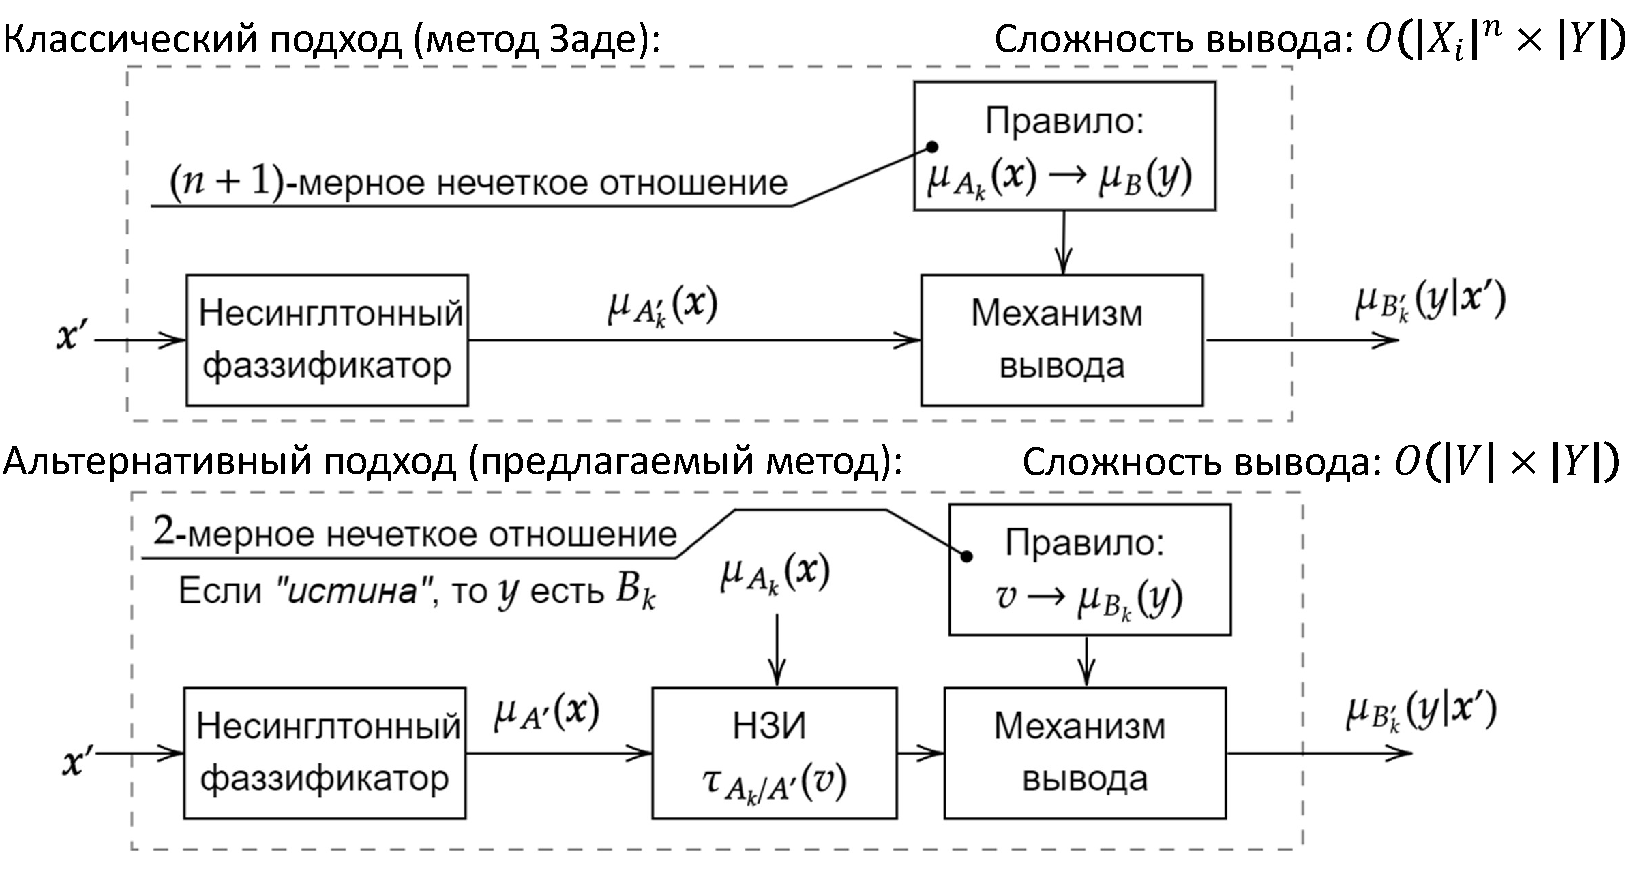
\includegraphics[scale=0.45]{ftv-schema-comparizon}
\caption{Сравнение классической схемы нечеткого вывода и схемы нечеткого вывода на основе НЗИ}
\label{fig:ftv-schema-comparizon}
\end{figure}

Порядок функции временной сложности вычисления $B'_k$ на основе выражения (\ref{eqn:ftv-compute-11}) составляет $O\left(n|V|^2+|V|\cdot |Y|\right)$, где $V=CP(A_k, A')$. Сравнение схем нечетких выводов с соответствии с соотношениями (\ref{eqn:fuz-problem-4}) и (\ref{eqn:ftv-compute-11}) представлены на рис. \cref{fig:ftv-schema-comparizon}.

\todo{\ul{Вывод типа Мамдани}}

В \cite{Sinuk2023} ослаблено ограничение на использование одной и той же $T$-нормы в формуле композиционного правила вывода в работах Менделя для случая вывода типа Мамдани, а также показано, что вывод по отдельному правилу в случае $T_2 = T_4 = T$ может быть записан через \textit{меру возможности}:
\begin{align*}
	\mu_{B'_k}(y) = \sup_{v\in[0;1]}\left\{\tau_{A_{k}|A'} \overset{\mathrm{T_2}}{\star} (v \overset{\mathrm{T_4}}{\star} \mu_{B_k}(y)) \right\} = \textstyle\prod_{\mathbf{A_k}|\mathbf{A'}} \overset{\mathrm{T}}{\star} \mu_{B_k}(y),
\end{align*}
где $\prod_{\mathbf{A_k}|\mathbf{A'}}=\sup_{v\in[0;1]}\left\{\tau_{A_{k}|A'} \overset{\mathrm{T}}{\star} v\right\}$.


Если при этом используется дефаззификация \textit{по центру сумм (CoS)} и $T$-норма Ларсена, то, как доказано в \cite{Sinuk2023}, результат дефаззификации зависит от ширины гауссовой или треугольной функции принадлежности консеквента, тогда как дефаззификация \textit{по среднему центру} учитывает только параметр центра. Например, при использовании в качестве выходной ф. п. гауссовой функции $\mu_{B_k}(y) = exp(-((y-\bar{y}_k)/\sigma_k)^2)$ формула дефаззификации имеет вид: 

\begin{equation}
	\hat{y}_{CoS} = \frac{\int_{\mathbb{Y}} y \sum_{k=1}^{N} \prod_{\mathbf{A_k}|\mathbf{A'}} \overset{\mathrm{T}_2}{\star} \mu_{B_k}(y)}{\int_{\mathbb{Y}} \sum_{k=1}^{N} \prod_{\mathbf{A_k}|\mathbf{A'}} \overset{\mathrm{T}_2}{\star} \mu_{B_k}(y)} = \frac{\sum_{k=1}^{N} \prod_{\mathbf{A_k}|\mathbf{A'}} \bar{y}_k \sigma_k}{\sum_{k=1}^{N} \prod_{\mathbf{A_k}|\mathbf{A'}} \sigma_k},
\end{equation}
поскольку $	\int_{-\inf}^{\inf}\mu_{B_k}(y) dy = \sigma_k \sqrt{\pi}$ и $\int_{-\inf}^{\inf} y \mu_{B_k}(y) dy = \bar{y}_k \sigma_k \sqrt{\pi}$.

Для предложенного метода вывода на основе нечеткого значения истинности в \cite{Karatach2024} показано, что для достаточно удаленных и непересекающихся выходных ф. п. нечетких множеств, т. е. когда $\mu_{B_k}(\bar{y}_r) = 0$ для $k \ne r$, сложность вычисления дефаззификации по центру тяжести сокращается за счет упрощения выражений импликаций:
\begin{itemize}
	\item для \textit{S}-импликации
	\begin{equation*}
		\hat{y}_{CoG} = \frac{\sum_{k=1}^{N} \overline{y}_k \Tnorm_{r=1}^N \left\{\sup_{v\in [0, 1]} \left\{\tau_{A_r|A'}\overset{\mathrm{T}_2}{\star}(1-v)\right\}\right\}}{\sum_{k=1}^{N} \Tnorm_{r=1}^N \left\{\sup_{v\in [0, 1]} \left\{\tau_{A_r|A'}\overset{\mathrm{T}_2}{\star}(1-v)\right\}\right\}},
	\end{equation*}
	\item для \textit{R}-импликации
	\begin{equation*}
		\hat{y}_{CoG} = \frac{\sum_{k=1}^{N} \overline{y}_k \Tnorm_{r=1}^N \left\{\tau_{A_r|A'}(0)\right\}}{\sum_{k=1}^{N} \Tnorm_{r=1}^N \left\{\tau_{A_r|A'}(0)\right\}},
	\end{equation*}
	\item для \textit{Q}-импликации
	\begin{equation*}
	{\fontsize{11}{6}
		\hat{y}_{CoG} = \frac{
			\sum_{k=1}^{N} \overline{y}_k \mathrm{T}_2 \left\{
			\sup_{v\in [0, 1]} \left\{\tau_{A_k|A'}\overset{\mathrm{T}_2}{\star}max(1-v, v)\right\}
			\Tnorm_{\substack{r=1\\r\ne k}}^N \left\{
			\sup_{v\in [0, 1]} \left\{\tau_{A_r|A'}\overset{\mathrm{T}_2}{\star}(1-v)\right\}
			\right\}
			\right\}
		}{
			\sum_{k=1}^{N} \mathrm{T}_2 \left\{
			\sup_{v\in [0, 1]} \left\{\tau_{A_k|A'}\overset{\mathrm{T}_2}{\star}max(1-v, v)\right\}
			\Tnorm_{\substack{r=1\\r\ne k}}^N \left\{
			\sup_{v\in [0, 1]} \left\{\tau_{A_r|A'}\overset{\mathrm{T}_2}{\star}(1-v)\right\}
			\right\}
			\right\}
		}.
	}
	\end{equation*}
\end{itemize}



\ul{Применение предложенного метода вывода в нечеткой модели для задачи классификации объектов}

Пусть производится классификация для набора объектов $\left\{q_l\right\}_{l=1}^M$, значения признаков которых значения признаков формализуются посредством термов лингвистических переменных, совокупность значений которых формирует вектор $\mathbf{x_l}=\left[x_{l1},\ldots,x_{ln}\right]$. Объекты классифицируются среди множества классов $\Omega = \left\{\omega_1, \dots, \omega_m\right\}$. Тогда база знаний нечеткой системы описывается набором из $N$ правил вида:
\begin{align*}
	R_k: \text{Если } \bigwedge_{i=1}^n \left(x_i\text{ есть }A_{ki}\right)\text{, то }\bigwedge_{j=1}^m \left(q\in\omega_j\,(\text{со степенью }\bar{z}_{kj})\right), k=\overline{1,N}.
\end{align*}
В этом правиле степень принадлежности объекта $q$ к классу $\omega_j$ задается значением $\bar{z}_{kj}$, которому можно поставить в соответствие значение лингвистической переменной $z_j$. Это значение выражается нечетким множеством имеющим в качестве базового множеств диапазон $[0,1]$, а в качестве функции принадлежности используется singleton:
\begin{equation}
\mu_{B_{kj}}(z_j) = \left\{
\begin{alignedat}{2}
	& 1, \quad & \text{eсли } z_j = \bar{z}_{kj} \\
	& 0, \quad & \text{eсли } z_j \ne \bar{z}_{kj}
\end{alignedat}
\right.
\end{equation}

Тогда при использовании дискретизированной дефаззификации по центру тяжести степень принадлежности объекта $q$ к $j$-му классу вычисляется по формуле:
\begin{align}
	\tau_{A_k|A'}(v) = \underset{i=\overline{1,n}}{\mathrm{\tilde{T}}} \left\{\mu_{CP(A_{ki}, A'_i)}(v_i)\right\}, k=\overline{1,N},\\
	\hat{z}_j = \frac{\sum_{r=1}^{N} \bar{z}_r \Tnorm_{k=1}^N \left\{\sup_{v\in [0, 1]} \left\{\tau_{\mathbf{A_k}|\mathbf{A'}}\overset{\mathrm{T}_2}{\star} I\left(v, \mu_{B_{kj}}(\bar{z}_r)\right)\right\}\right\}}{\sum_{r=1}^{N} \Tnorm_{k=1}^N \left\{\sup_{v\in [0, 1]} \left\{\tau_{\mathbf{A_k}|\mathbf{A'}}\overset{\mathrm{T}_2}{\star} I\left(v, \mu_{B_{kj}}(\bar{z}_r)\right)\right\}\right\}}.
\end{align}

%\begin{figure}[th]
%	\centering
%	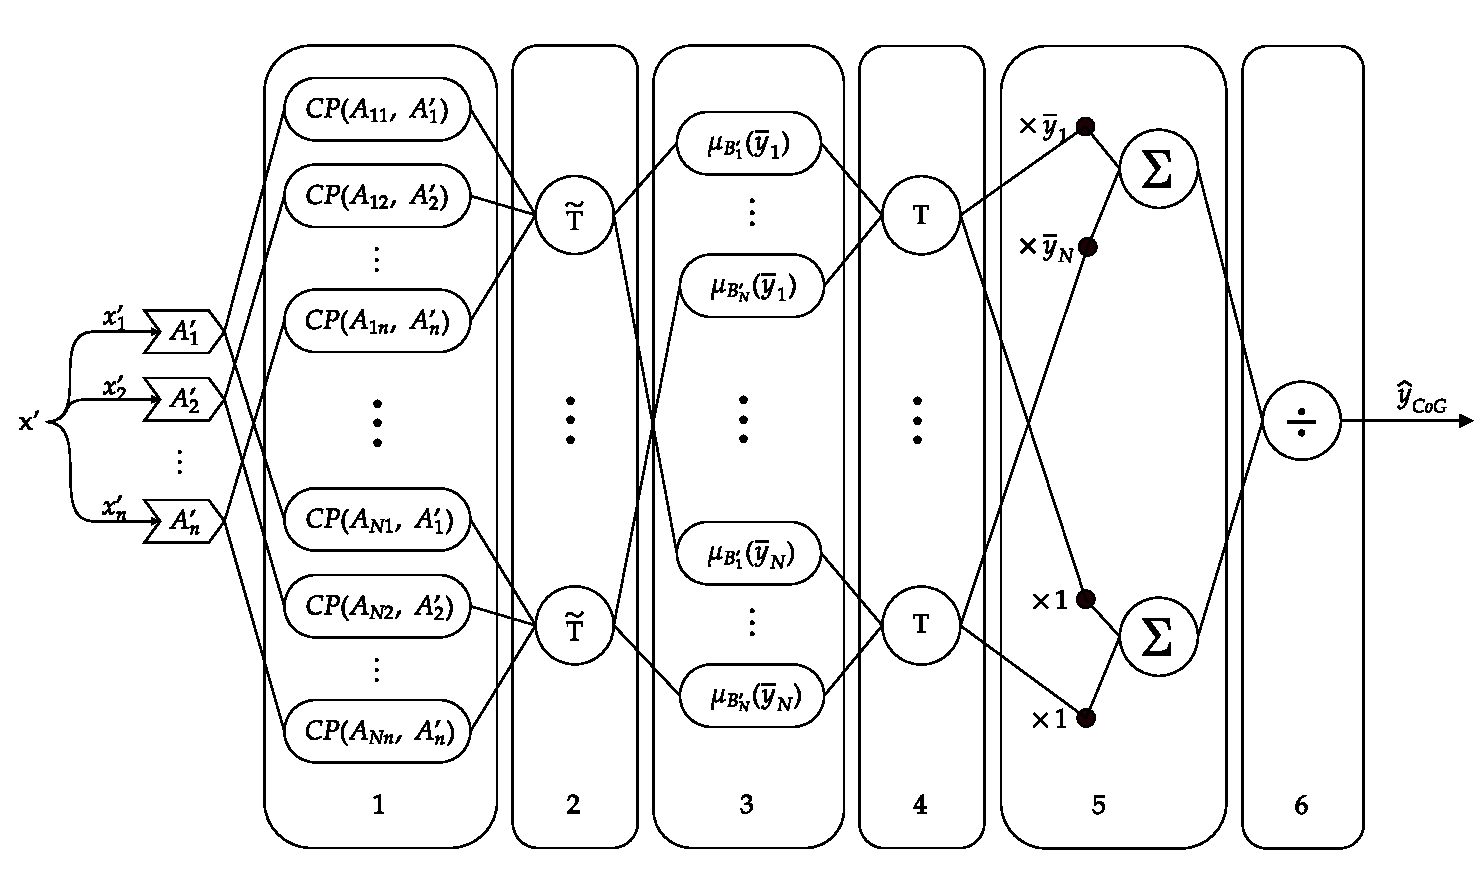
\includegraphics[scale=0.5]{neurofuzzysystem-defuzzification-cog}
%	\caption{Схема нейро-нечеткой системы с использованием дефаззификации по методу центра тяжести}
%	\label{fig:neurofuzzysystem-defuzzification-cog}
%\end{figure}



\ul{Применение предложенного метода вывода в нечеткой модели для задачи регрессии временных рядов}

Пусть задан временной ряд $\left\{y_t\right\}_{t=1}^T = \left\{y_1, \dots, y_T\right\}$, где $y_t \in \mathbb{R}$ --- измеренное значение наблюдаемой переменной в момент времени $t$, а $T$ --- длина доступной выборки. При моделировании временных последовательностей с использованием нейро-нечетких систем каждое значение $y_t\in \mathbb{Y}\subseteq \mathbb{R}$ фаззифицируется в нечеткое множество $A'_t$. Тогда для прогнозирования значения $\hat{y}_{t+h}$ с горизонтом $h$ на основании среза наблюдений $y_{t-p+1}, \dots, y_t$ можно использовать нечеткую систему с базой из $N$ правил вида:
\begin{align*}
	R_k: \text{Если } \bigwedge_{i=1}^p \left(y_{t-i+1}\text{ есть }A_{ki}\right)\text{, то }y_{t+1}\textrm{ есть }A_{k\,p+1}, k=\overline{1,N},
\end{align*}
где $p$ --- размер окна запаздывания (порядок модели, количество входов нечеткой системы).

В задаче регрессии дискретная формула дефаззификации по центру тяжести не показывает достаточной точности, а непрерывная ее формулировка имеет большую вычислительную сложность. Поэтому в работе для регрессии используется дефаззификация по среднему максимуму:

\begin{align}
	\tau_{A_k|A'}(v) = \underset{i=\overline{1,n}}{\mathrm{\tilde{T}}} \left\{\mu_{CP(A_{ki}, A'_{t-p+i})}(v_i)\right\}, k=\overline{1,N},\\
	\hat{y}_{t+h} = \argmax_{y\in\mathbb{Y}} \left\{\Tnorm_{k=1}^N \left\{\sup_{v\in [0, 1]} \left\{\tau_{\mathbf{A_k}|\mathbf{A'}}\overset{\mathrm{T}_2}{\star} I\left(v, \mu_{A_{k\,p+1}}(y)\right)\right\}\right\}\right\}.
\end{align}

\begin{figure}[thb]
	\centering
	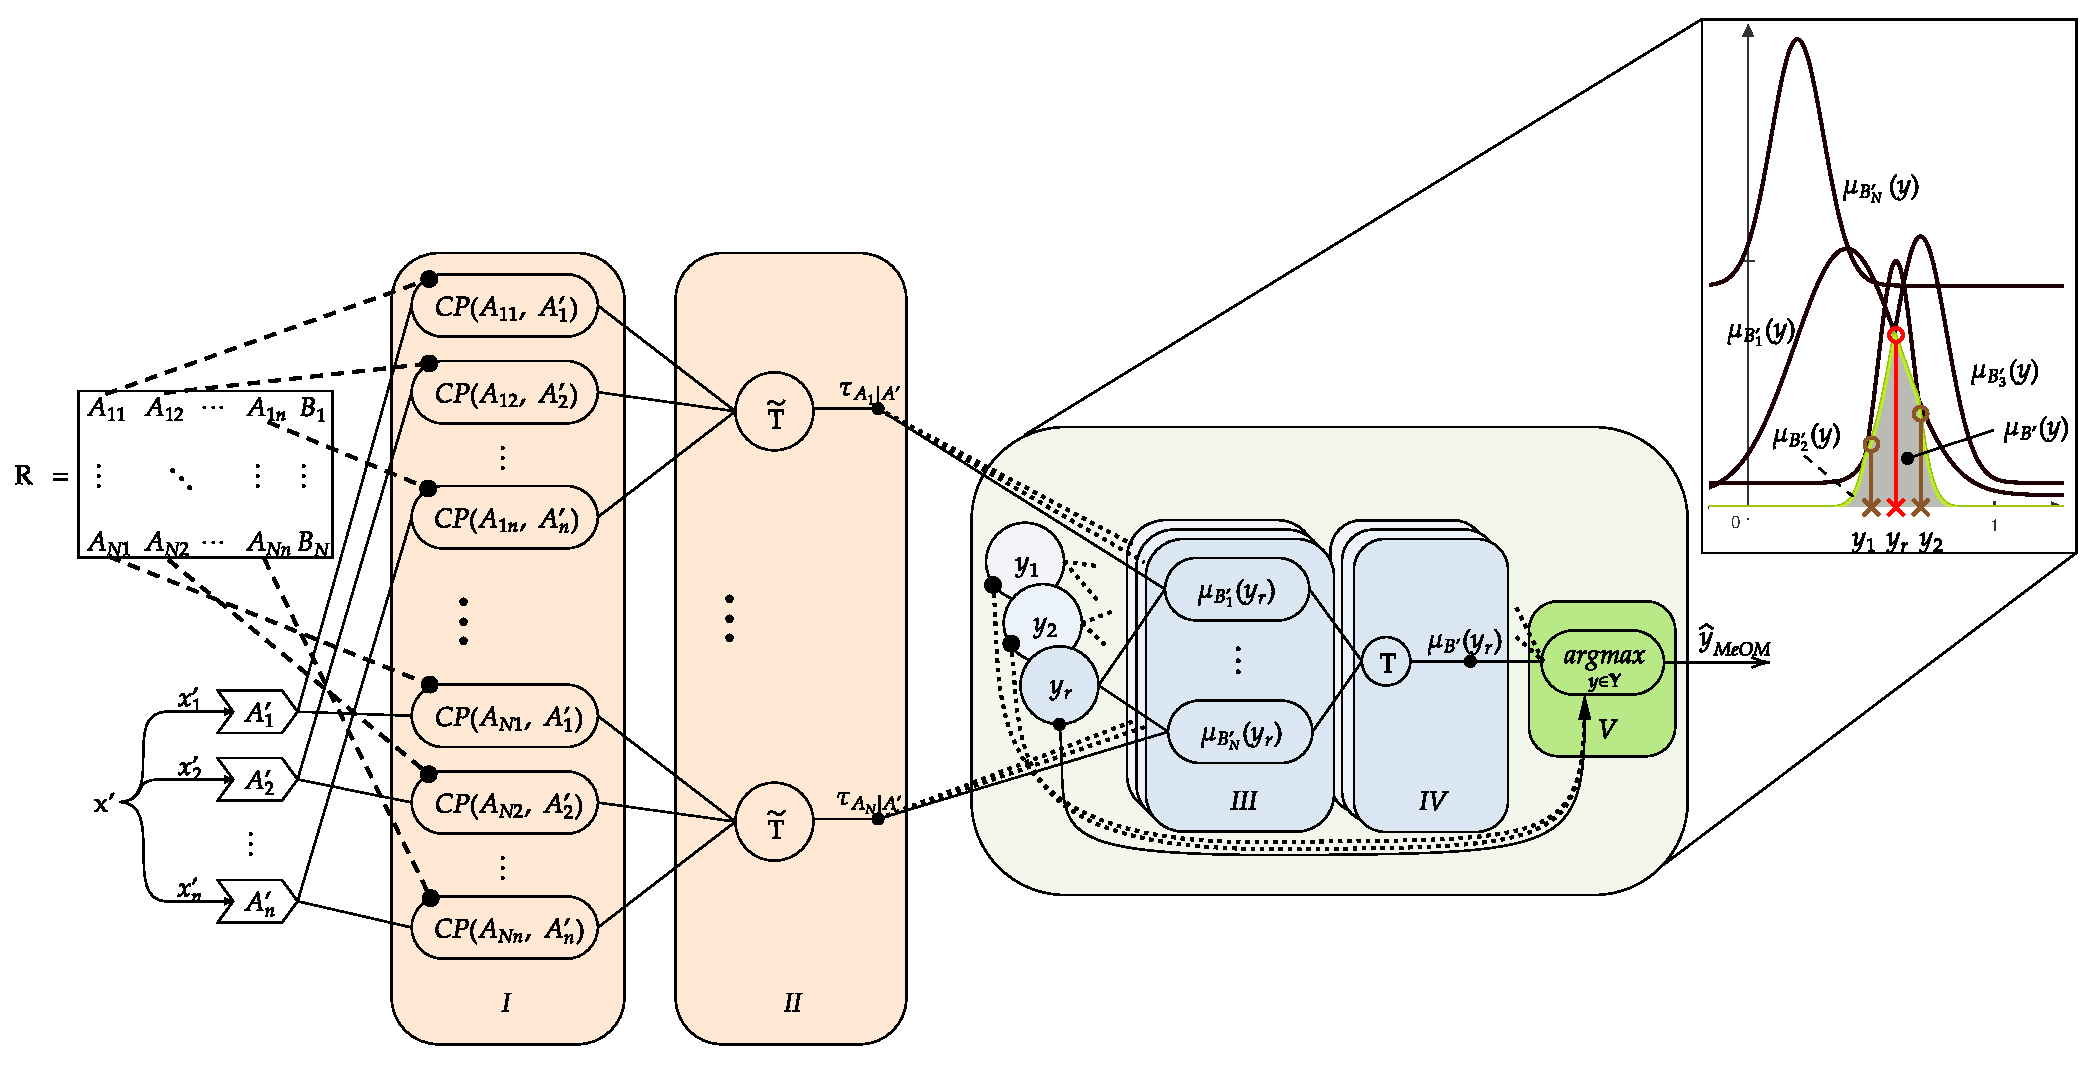
\includegraphics[width=\linewidth]{nfs-ftv-and-defuz-meom-with-defuz-demo}
	\caption{Схема нейро-нечеткой системы с вычислением НЗИ и дефаззификацией по среднему максимуму, а также пример работы дефаззификации.}
	\label{fig:nfs-ftv-and-defuz-meom-with-defuz-demo}
\end{figure}





%Нейро-сетевая структура изображена на рисунке 

%\begin{figure}[ht]
%	\centering
%	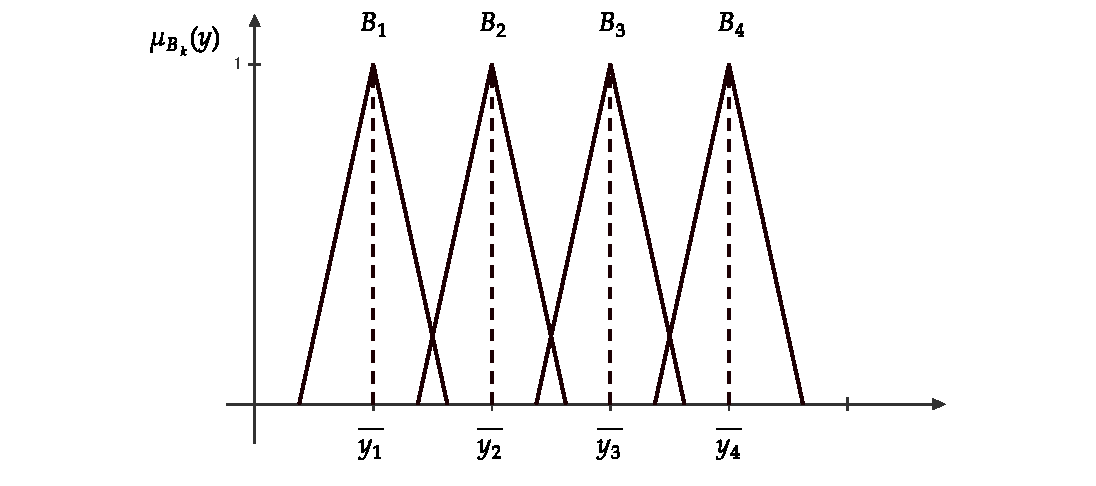
\includegraphics[scale=0.5]{out-mf-with-low-crossing}
%	\caption{Пример нечетких множеств, удовлетворяющих условию $\mu_{B_k}(y_r) = 0$ для $y \ne r$.}
%	\label{fig:out-mf-with-low-crossing}
%\end{figure}



\textbf{Третья глава} посвящена выработке эффективной параллельной реализации разработанного метода нечеткого вывода на основе нечеткого значения истинности с использованием технологии CUDA. В главе описан ключевые особенности организации вычисления нечеткого вывода при использовании технологии CUDA, параллельный алгоритм свертки НЗИ, особенности реализации методов дефаззификации в нечеткой модели регрессии и схема ускоренного вывода регрессионной нечеткой системы за счет предварительного отбора правил с ближайшими антецедентами.

\ul{Параллельный алгоритм свертки НЗИ}

При программной реализации вычисления и свертки НЗИ $\tau_{A_{ki}|A'_i}$ вычисление производится в точках расчетной сетки. \ul{Значение НЗИ по $i$-му входу в точке расчетной сетки $v_j$ в данной работе обозначается $ftv_i[v_j]$ (\textit{ftv --- fuzzy truth value}).} Расчетная сетка размера $D_{ftv}$ задается на пространстве $\mathbb{V}=[0;1]$ мощности $|\mathbb{V}|$.

Для нахождения свертки НЗИ по одному правилу можно составить алгоритм на основе формулы (\ref{eqn:ftv-compute-10}). Вычислительная сложность при параллельной реализации такого алгоритма составит $O\left(D_{ftv}^2 \cdot \log{n}\right)$. Значения $ftv_i[v_j]$ необходимо вычислить до запуска алгоритма свертки, что потребует сложности по памяти $O\left(D_{ftv}\cdot n\right)$.

\begin{algorithm}
	\begin{algorithmic}
		\Require $ftv_i,\ i=\overline{1,n}$ --- это $\tau_{A_{ki}|A'_i}$ дискретизированная в точках $v_j$
		\State $max\_ftv[i] = 0;$
		\For{$v_j = 1\dots0$}
		\State $s \gets \left\{ftv_i[v_j] \mid ftv_i[v_j] >= max\_ftv[i]\right\};$
		\State $max\_ftv[i] \gets max(max\_ftv[i], ftv_i[v_j]);$
		\State $v\_max\_index \gets \mathrm{arg\,max}_i\left\{ftv_i[v_j]\right\};$
		\If{$s = \emptyset \And i = v\_max\_index$}
		\State $r[i] \gets ftv_{i}[v_j];$
		\Else
		\State $r[i] \gets max\_ftv[i];$
		\EndIf
		\State $ftv\_reduced[v_j] \gets \underset{i}{T_3}\left\{r[i]\right\}$;
		\EndFor
		\State \Return $ftv\_reduced$
	\end{algorithmic}
	\caption{Алгоритм свертки НЗИ при $T_1=min$}
	\label{alg:ftv-reduction}
\end{algorithm}

\begin{figure}[ht]
	\centering
	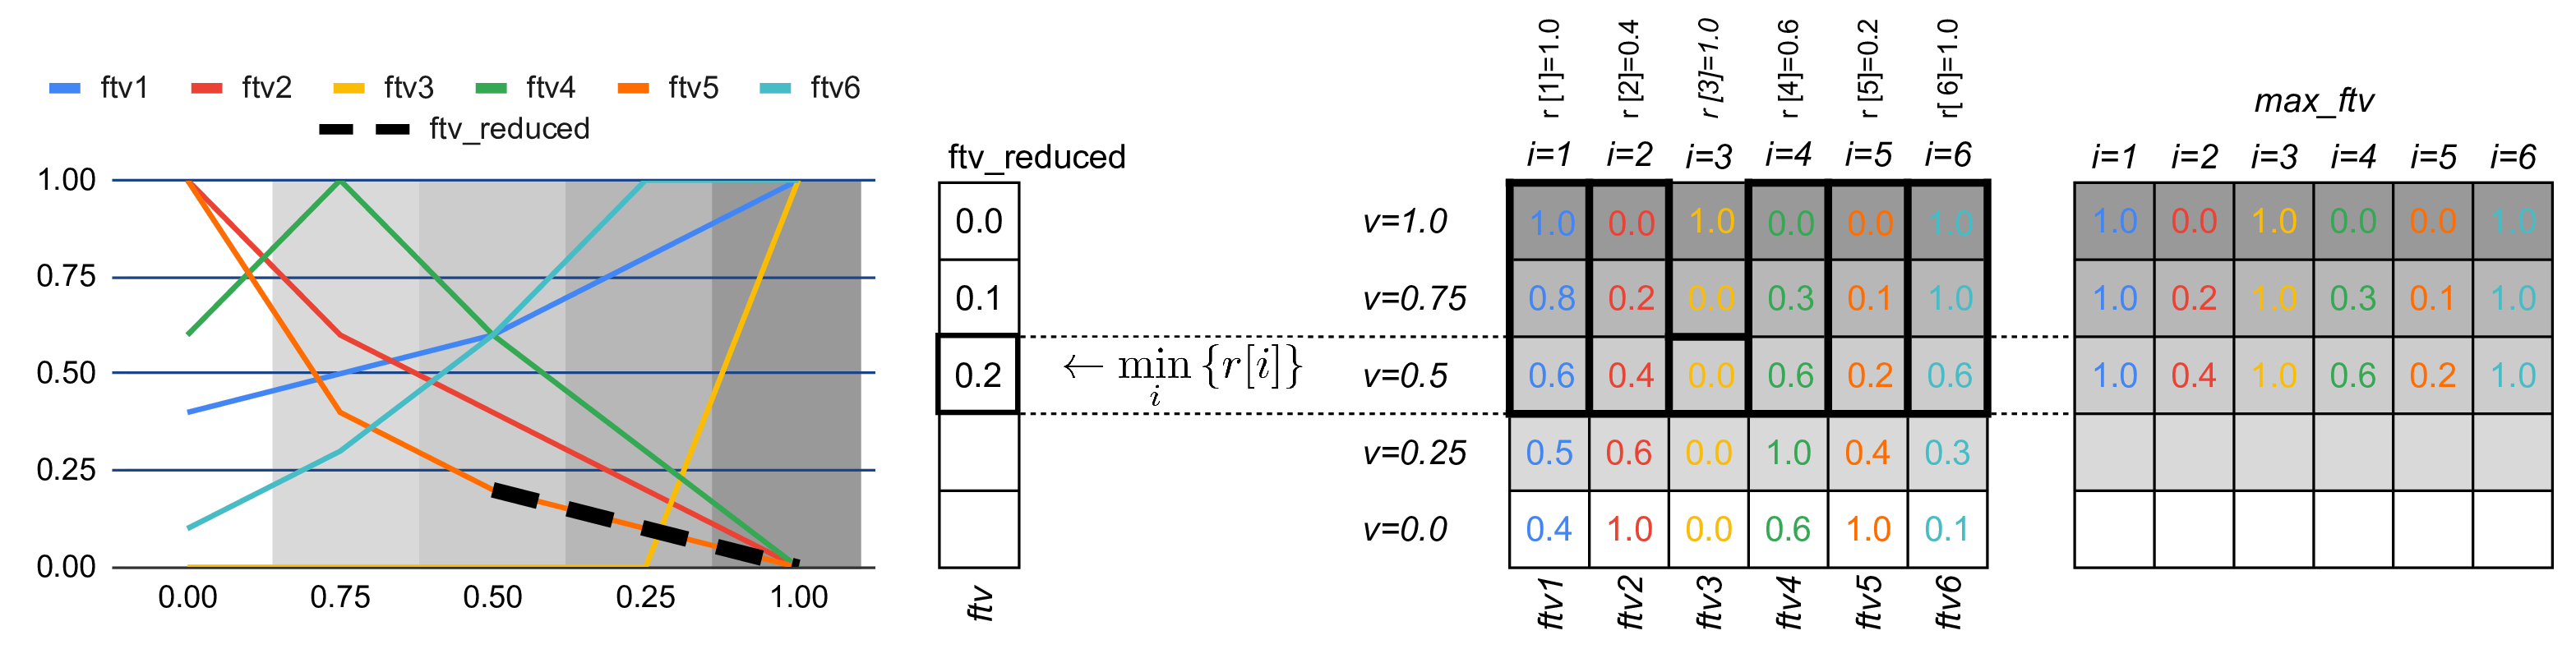
\includegraphics[width=\textwidth]{ftvs-reduction-example-gradient}
	\caption{Пример работы параллельного алгоритма свертки НЗИ при расчетной сетке состоящей из 5 точек.}
	\label{fig:ftvs-reduction-example}
\end{figure}

При выполнении работы был разработан параллельный алгоритм свертки НЗИ \cite{Karatach2023b} с вычислительной сложностью $O\left(D_{ftv}\cdot \log{n}\right)$. Алгоритм \ref{alg:ftv-reduction} разработан при допущении, что $T_1 = min$, тогда $\underset{i=\overline{1,n}}{\mathrm{T_1}}v_i = \min_{i=\overline{1,n}} v_i$ в формуле (\ref{eqn:ftv-compute-8}). При работе алгоритм итеративно продвигается от 1 к 0 в области $\mathbb{V}$, как показано на рисунке \cref{fig:ftvs-reduction-example}. На каждой $j$-й итерации вычисляются значения $ftv_i[v_j]$, которые агрегируются в одном вспомагательном массиве \textit{max\_ftv}, который требует сложности по памяти $O\left(n\right)$.

%При дискретизированном вычисление ф. п. свертки НЗИ в некоторой точке расчетной сетки $v_j\in [0,1]$ потребуется просматривать значения НЗИ в отрезке $[v_j, 1]$, то есть имеет вычислительную сложность $O(D_{ftv})$, где $D_{ftv}$ --- число точек расчетной сетки ф. п. НЗИ. Таким образом вычисление свертки НЗИ по формуле (\ref{eqn:ftv-compute-11}) может быть распараллелено по точкам расчетной сетки, а нахождение $\tau_{\mathbf{A_k}|\mathbf{A'}}(v_j)$ использует операцию свертки, которая в имеет ограниченную возможность распараллеливания, но в целом требует большого количества повторных вычислений значений $\tau_{A_{ki}|A'_i}(v_k), v_k\in [v_j, 1]$. В \ref{alg:ftv-reduction} \cite{} предложен алгоритм вычисления свертки НЗИ сразу по всем входам с использованием техники динамического программирования, имеющий линейную зависимость от размера расчетной сетки $D_{ftv}$..


\ul{Библиотека с параллельной реализацией нечеткого вывода на основе технологии CUDA}

Для более оперативного проведения экспериментов и практического применения в нагруженных промышленных приложениях была выполнена параллельная реализация нечеткого вывода на основе НЗИ с использованием языка программирования С++ и технологии CUDA. Для удобства использования к разработанному модулю вывода был реализован интерфейс из языка Python с помощью расширения Cython. Схема использования изображена на рисунке \cref{fig:application-schema-diagram}.

Важным достоинством реализации является полная организация вычислений внутри \textit{потоковых мультипроцессоров} графических ускорителей за счет размещения всей базы правил и пакета экземпляров входных данных в разделяемой памяти на чипе потокового мультипроцессора, что предотвращает возникновение простоя арифметико-логических модулей при ожидании загрузки порции данных (например, базы правил) из глобальной памяти графического ускорителя. Также, вычисления организованы внутри группы из 32 CUDA-нитей, что избавляет от необходимости синхронизации внутри CUDA-блока и позволяет использовать инструкции аппаратной свертки массивов чисел внутри таких групп.

В библиотеке реализована дискретизированная дефаззификация по центру тяжести и дефаззификация по среднему максимуму. Для точного вычисления значения дефаззификации выхода нечеткой системы для задачи регрессии используется метод оптимизации \textit{Gradient-aware Particle Swarm Optimization}.

\begin{figure}[ht]
	\centering
	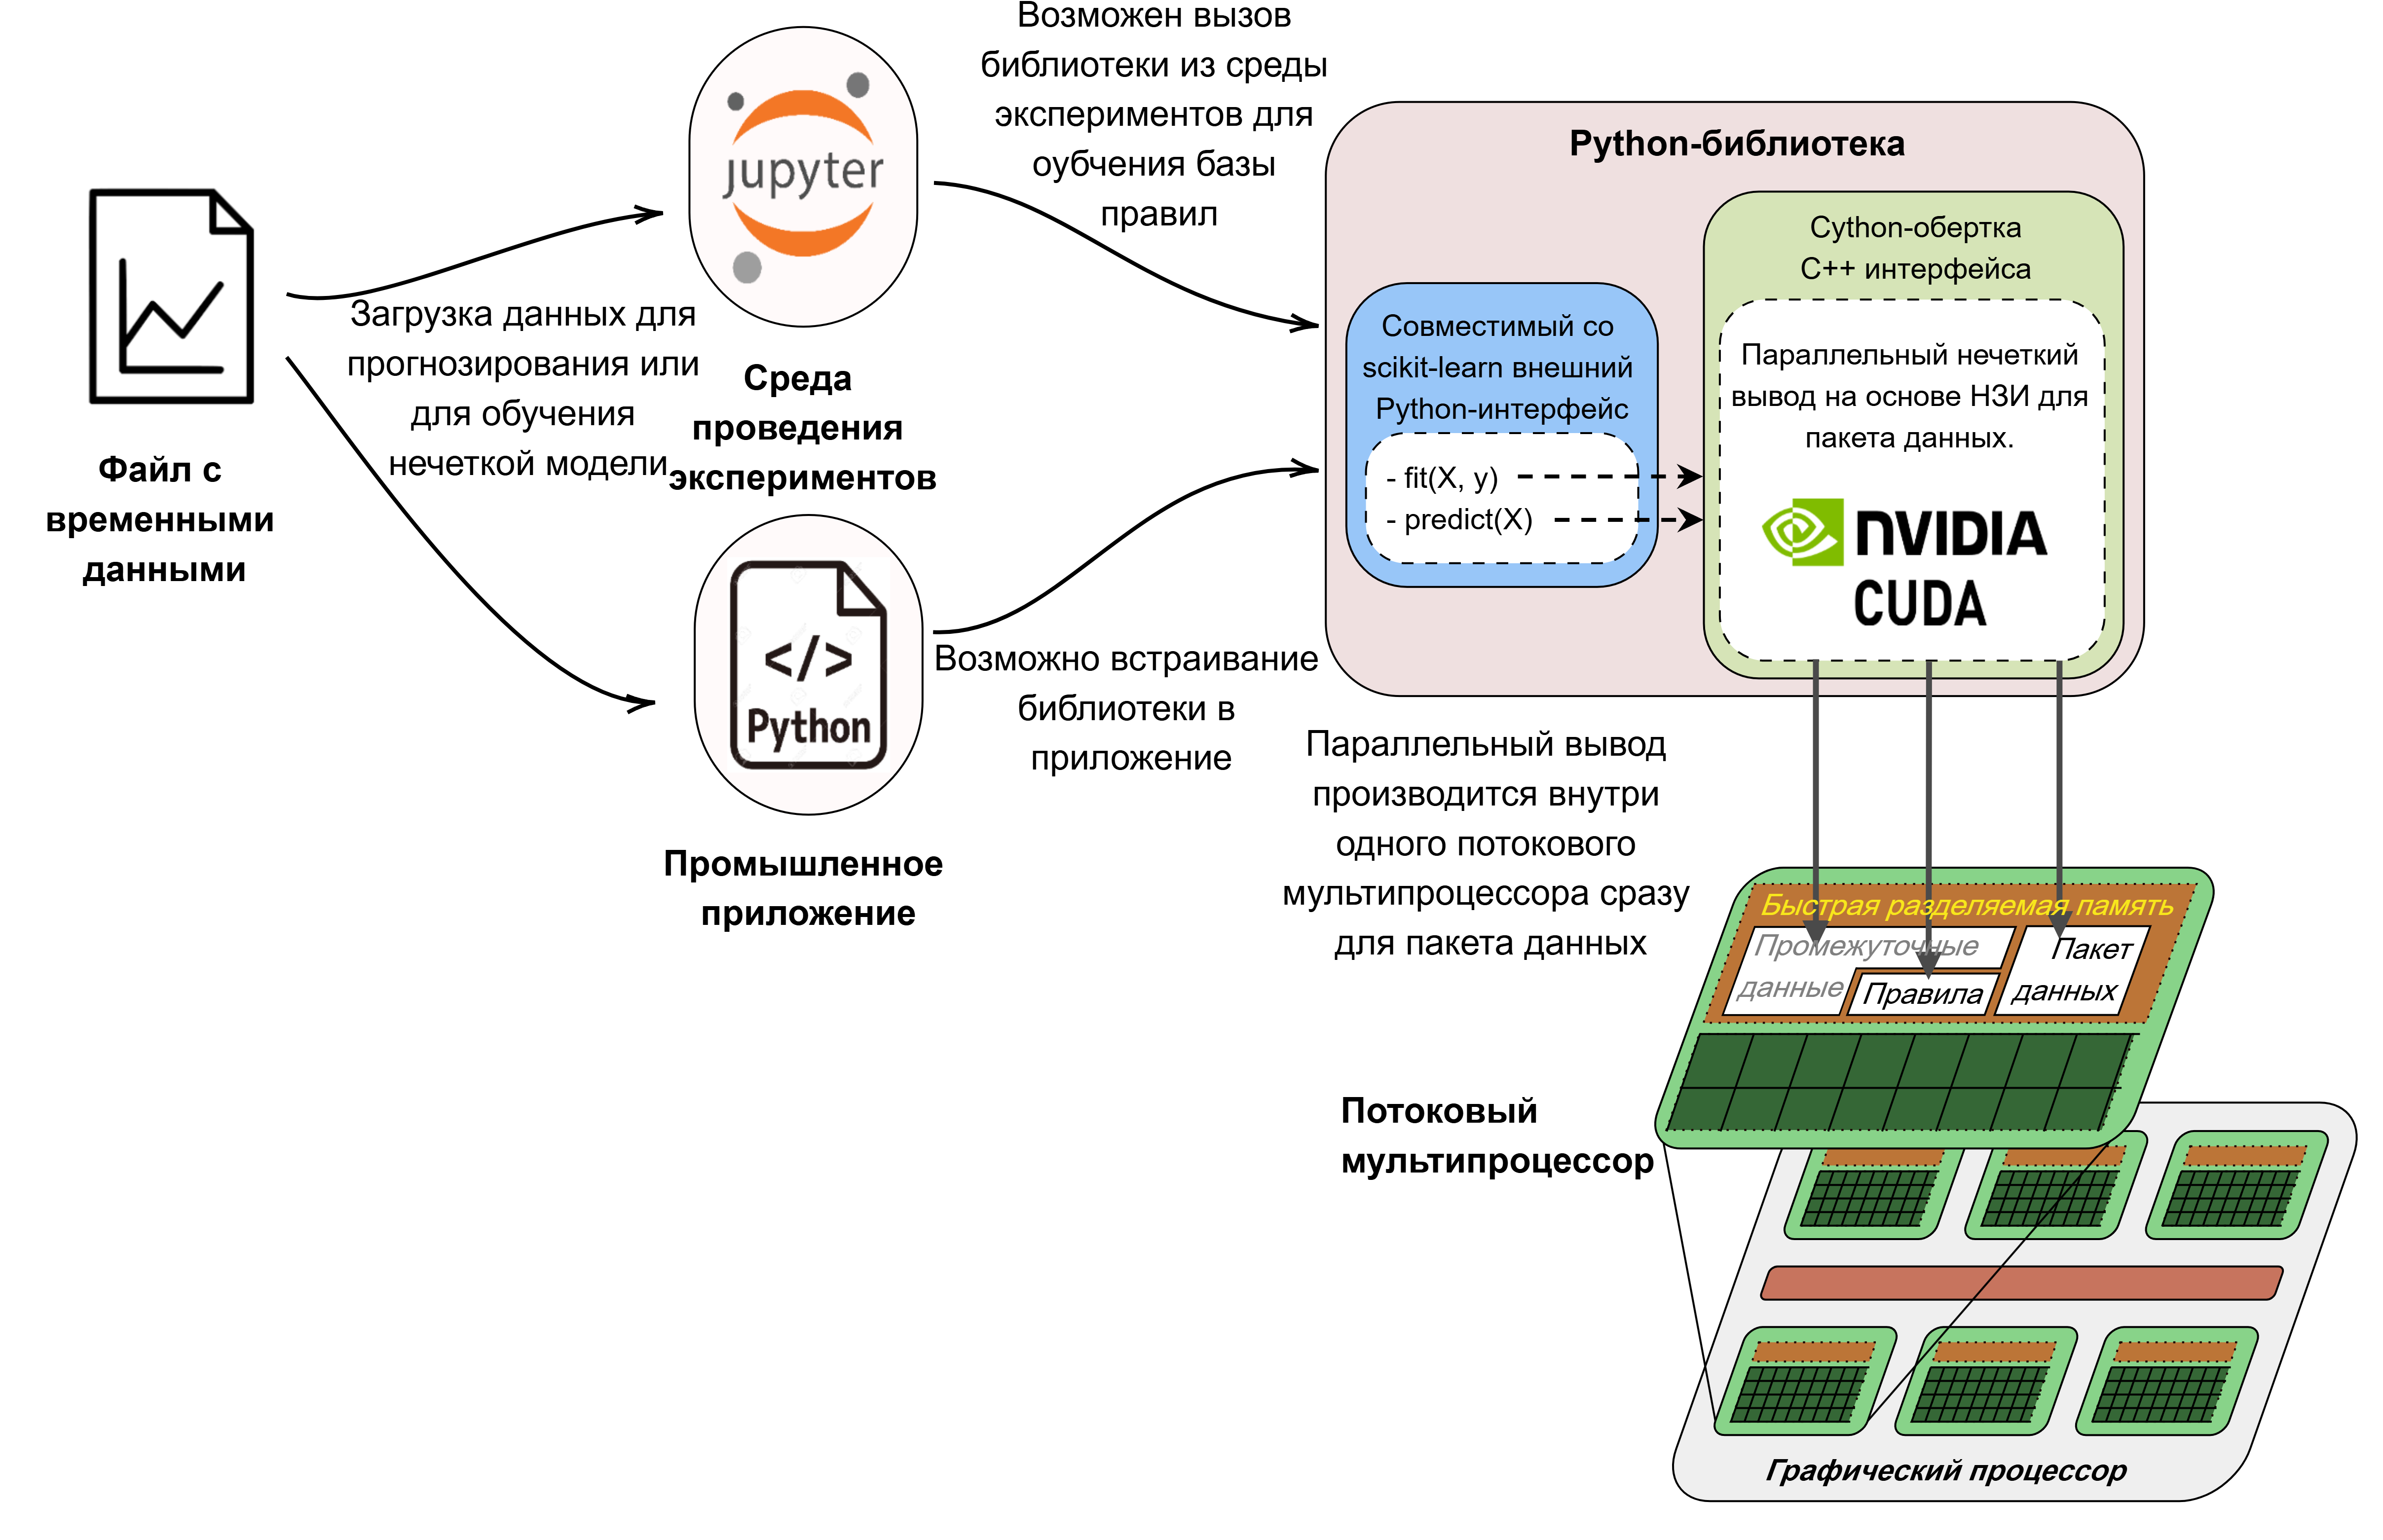
\includegraphics[width=\linewidth]{application-schema-diagram}
	\caption{Схема использования библиотеки для нечеткого моделирования и прогнозирования временных рядов.}
	\label{fig:application-schema-diagram}
\end{figure}

\textbf{Четвёртая глава} содержит описание нескольких проведенных экспериментов для оценки характеристик разработанной нечеткой модели прогнозирования временных рядов. Первый эксперимент направлен на подтверждение полиномиальной зависимости времени нечеткого вывода от количества входов нечеткой системы, а также на прирост качества прогнозирования при использовании нечеткого вывода логического типа с несинглтонной фаззификацией. Второй эксперимент был проведен для оценки качества в прикладной задаче прогнозирования временных рядов.

Первый эксперимент проводился с использованием синтетического набора данных Mackey-Glass (M-G). В данной работе этот набора данных был сгенерирован в результате решения дифференциального уравнения:
\begin{equation}
	\frac{dx(t)}{dt} = \beta\frac{x(t-\tau)}{1+x(t-\tau)^n}-\gamma x(t)
	\label{eqn:mackey-glass-definition},
\end{equation}
со значениями параметров $\tau = 30, \beta = 0.2, \gamma = 0.1$.

В эксперименте использовался участок временного ряда $t=\overline{1,1000}$, а также применялся адаптивный метод оценки зашумленности временной последовательности в каждой точке $t$ на основе экспоненциально взвешенного скользящего среднего.

\begin{figure}[ht]
	\begin{minipage}[c]{0.49\textwidth}
		\centering
		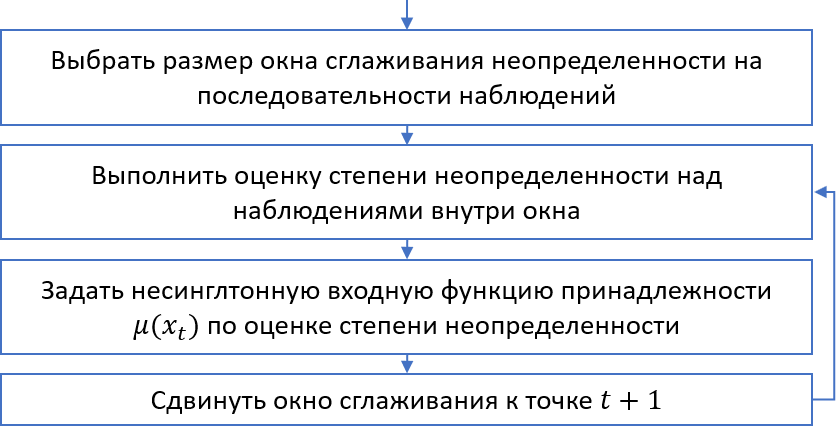
\includegraphics[width=\textwidth]{ns-procedure}
		\caption{Схема обобщенной процедуры адаптивной несинглтонной фаззификации временной последовательности.}
		\label{fig:ns-procedure}
	\end{minipage}
	\hfill
	\begin{minipage}[c]{0.49\textwidth}
		\centering
%		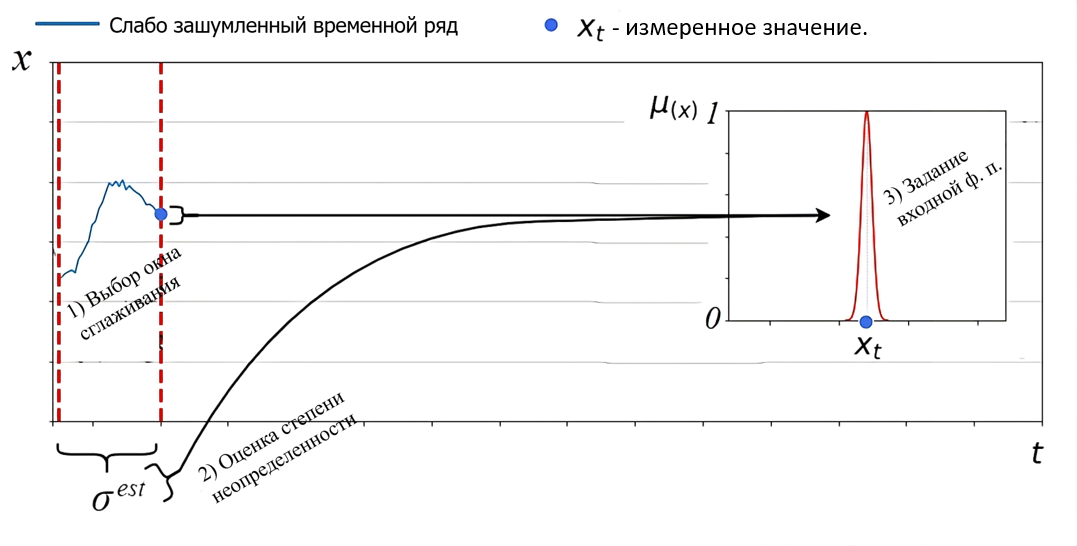
\includegraphics[width=\textwidth]{ns-demo-low-noise}
%		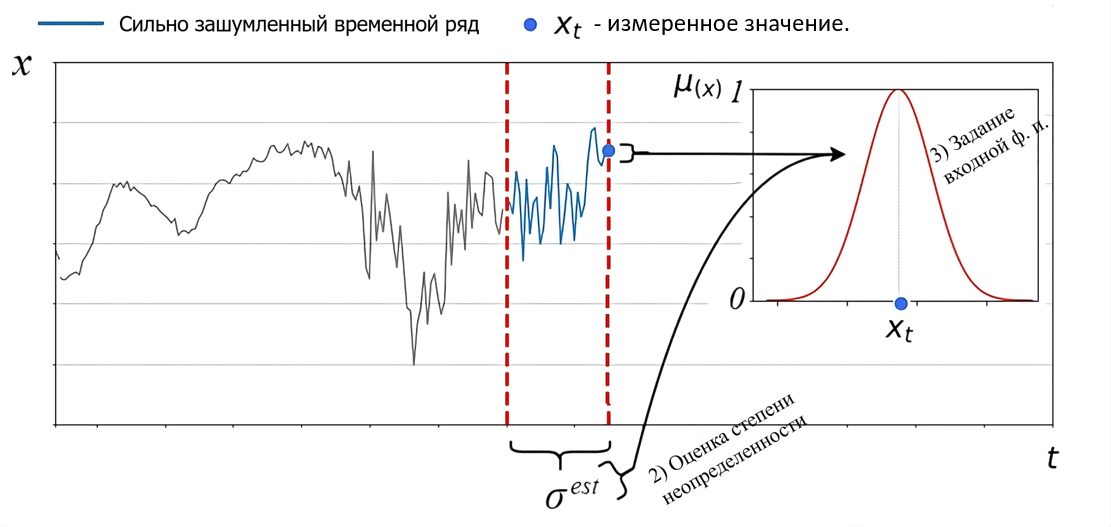
\includegraphics[width=\textwidth]{ns-demo-large-noise}
		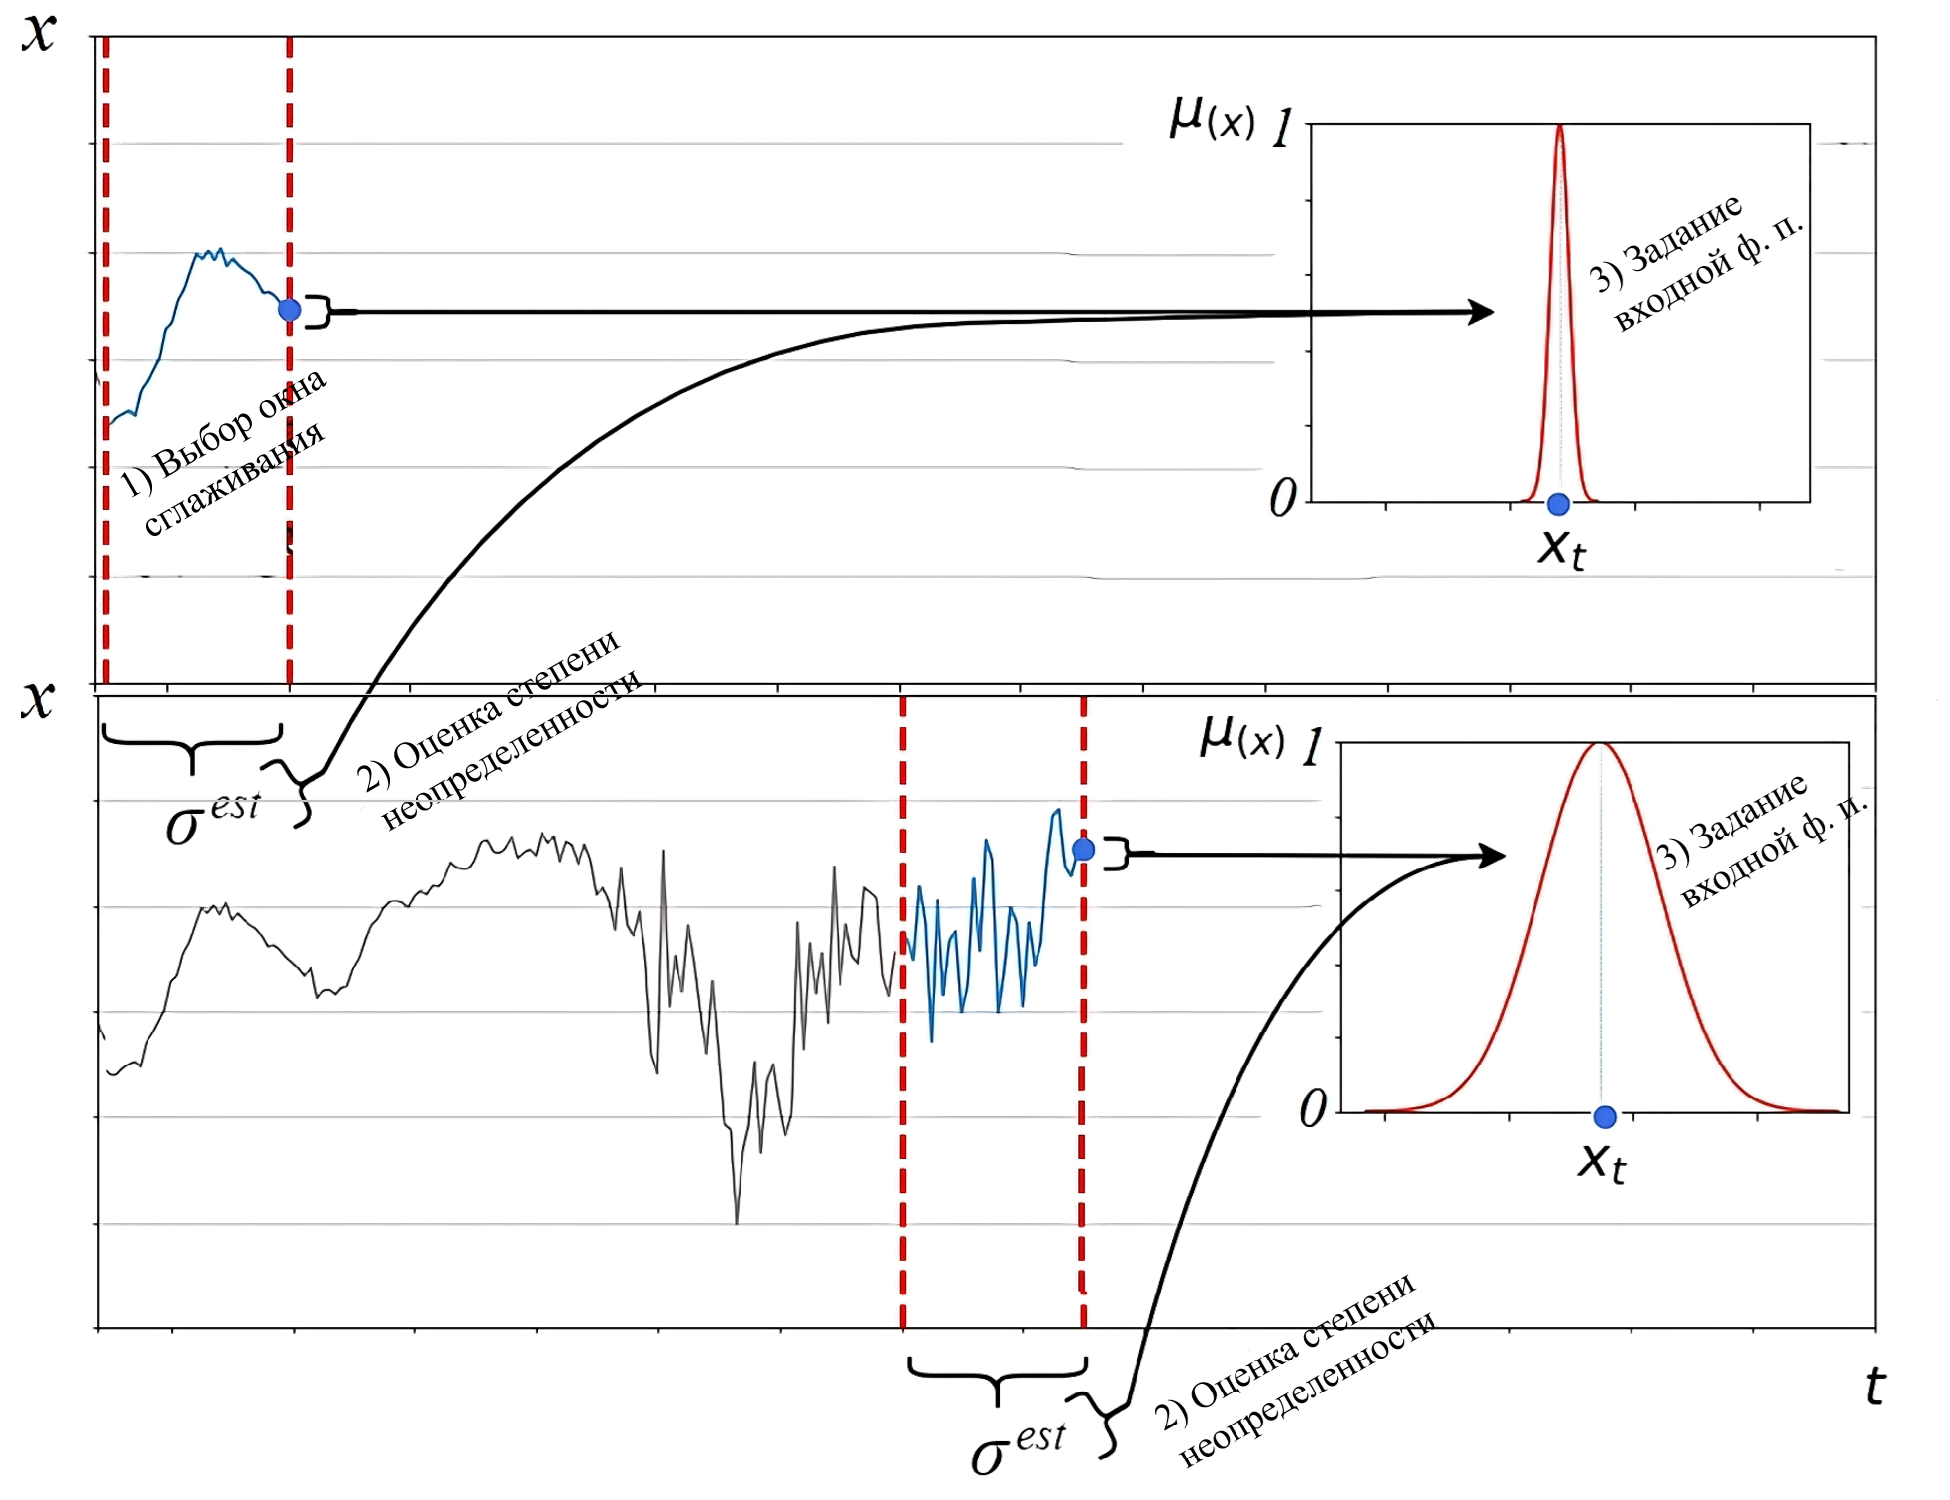
\includegraphics[width=\textwidth]{ns-demo-low-and-high-noise}
		\caption{Иллюстрация процедуры несинглтонной фаззификации временного ряда с низким (вверху) и высоким (внизу) уровнем шума.}
		\label{fig:ns-demo-low-and-high-noise}
	\end{minipage}
\end{figure}

Нечеткие множества для значений временного ряда были получены с использованием этой процедуры фаззификации временных рядов (\cref{fig:ns-procedure}) для обеспечения адаптивности оценки неопределенности в конкретной точке. Формулы для вычисления степени неопределенности показаны ниже%

\begin{minipage}{0.45\linewidth}
\begin{align}
	\label{eqn:mackey-glass-seq-diff}
	d_1 &= d_2, \notag \\
	d_t &= \frac{1}{\sqrt{2}}(x_t - x_{t-1}),
\end{align}
\begin{align}
	\hat{d}_t &= (1-\alpha) \hat{d}_{t-1} + \alpha d_t \notag \\
	&= \sum_{p=1}^t \alpha (1-\alpha)^{t-p} d_p. %\notag
	\label{eqn:mackey-glass-seq-diff-mean}
\end{align}
\end{minipage}\hfill
\begin{minipage}{0.45\linewidth}
\begin{align}
	\hat{\sigma}^2_t &= (1-\alpha) \hat{\sigma}^2_{t-1} + \alpha (d_t - \hat{d}_t) \notag \\
	&= \sum_{p=1}^t \alpha (1-\alpha)^{t-p} (d_p - \hat{d}_p)^2, \label{eqn:mackey-glass-seq-diff-var-iterative} \\
	\hat{\sigma}_t &= \sqrt{\hat{\sigma}^2_t}, \label{eqn:mackey-glass-seq-diff-std}
\end{align}
\end{minipage}

\begin{figure}[ht]
	\centering
	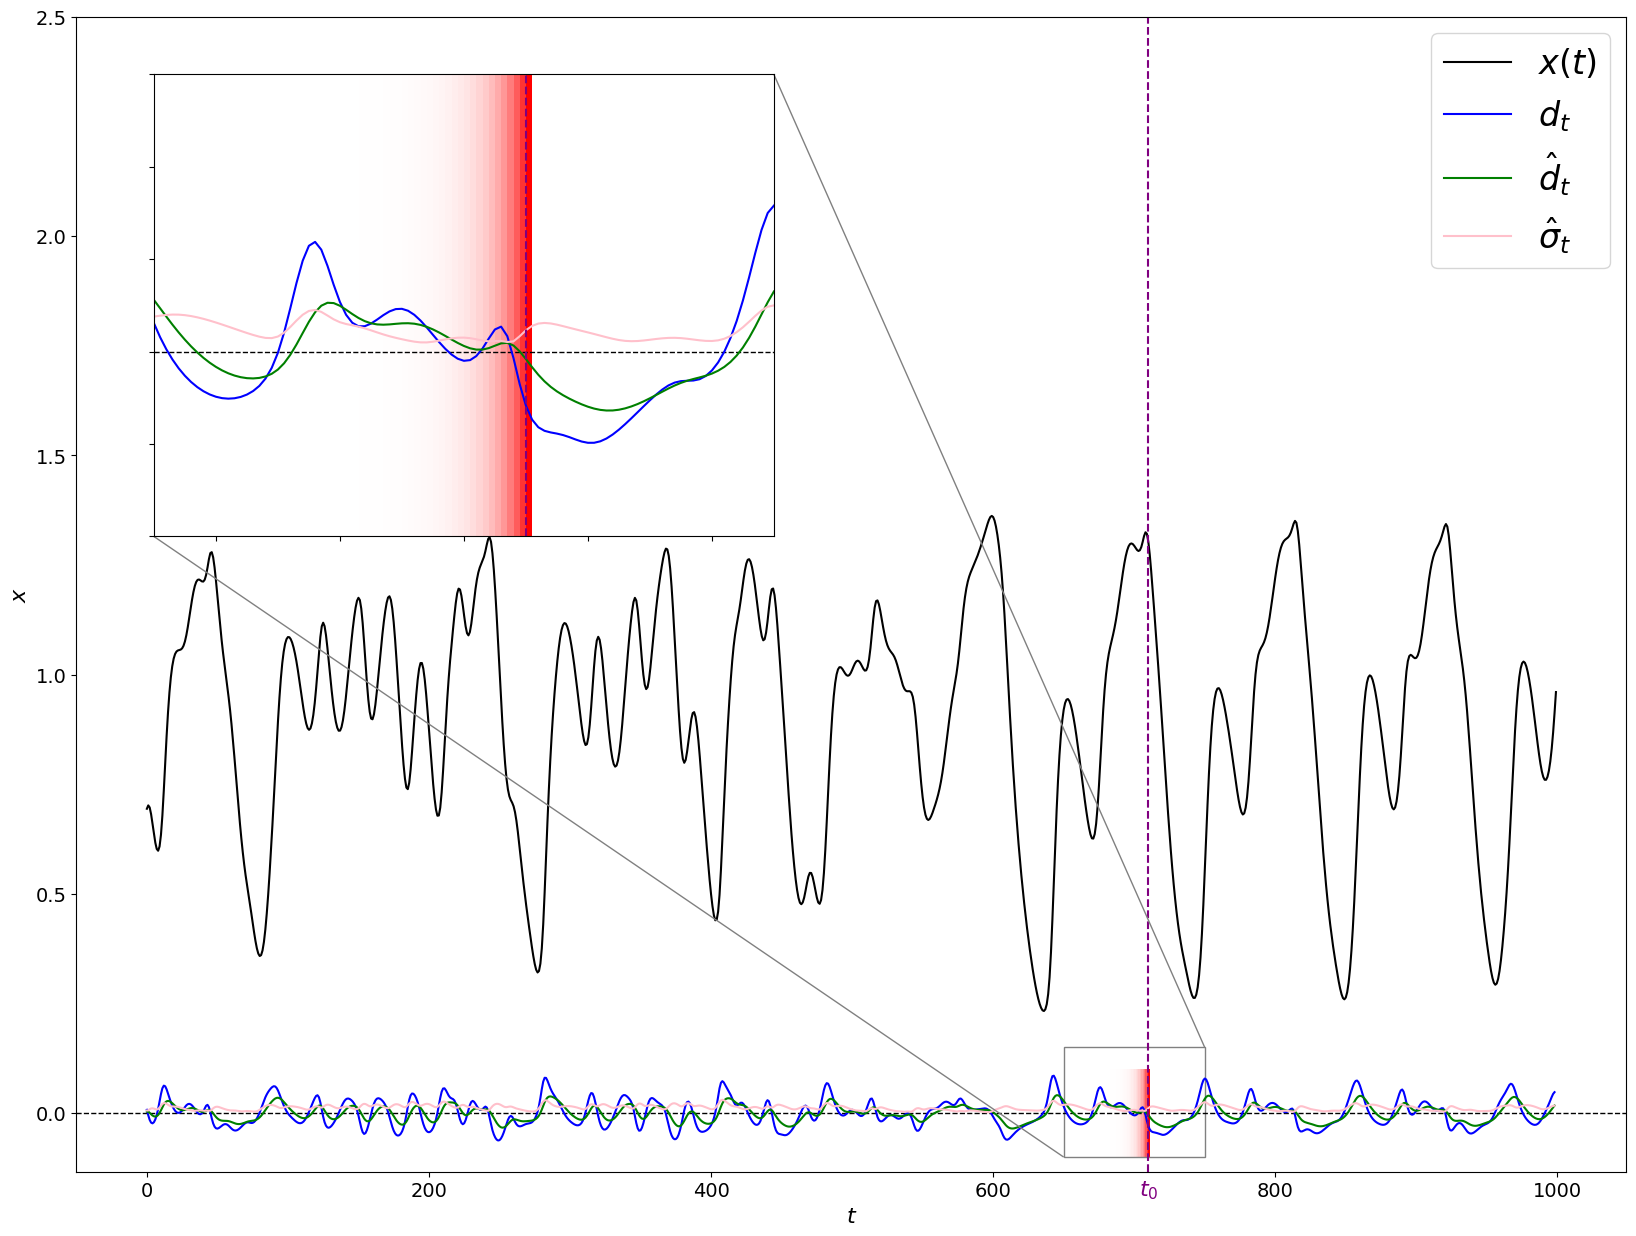
\includegraphics[scale=0.3]{mackey-glass-ewma-example}
	\caption{График сгенерированной последовательности Mackey-Glass $x(t), t\in[0;999]$, график разностей соседних точек $d_t$ последовательности $x(t)$, график $\hat{d}_t$ с наложением экспоненциально взвешенного сглаживания на последовательность разностей и график экспоненциально взвешенного скользящего среднеквадратичного отклонения разностей $\hat{\sigma}_t$. На вложенном изображении участка $t\in[650,750]$ яркостью красного цвета показано значения весового коэффициента $\alpha (1-\alpha)^{t-p}, p=\overline{1,t_0}$ при $\alpha = 0.2$.}
	\label{fig:mackey-glass-ewma-example}
\end{figure}

\begin{figure}[tbh]
	\centering
	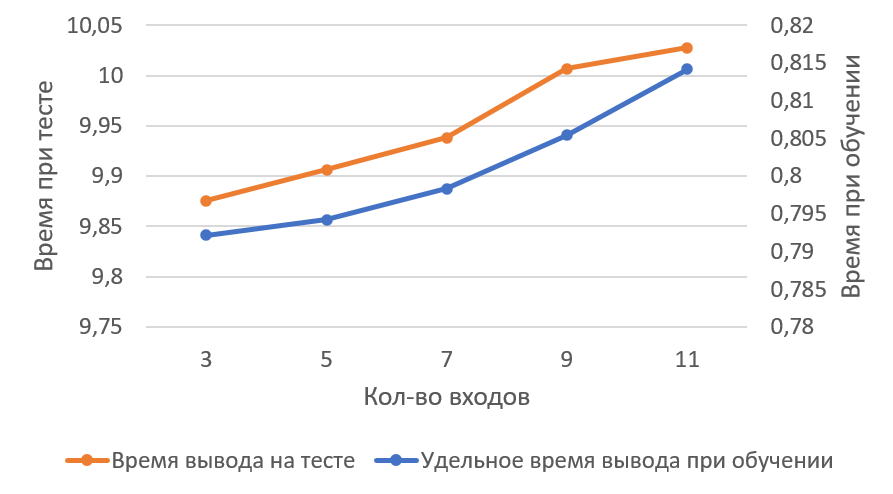
\includegraphics[scale=0.7]{mackey-glass-inference-duration}
	\caption{График длительности выполнения параллельной реализации нечеткого вывода для обучающего и тестового набора данных при количестве правил $N=30$.}
	\label{fig:mackey-glass-inference-duration}
\end{figure}

После проведенного вычислительного эксперимента были получены показатели удельного (на одну точку из набора точек одной итерации алгоритма PSO) времени работы параллельного алгоритма нечеткого вывода на основе НЗИ на обучающем наборе данных и времени работы на тренировочном наборе данных для различного размера окна запаздывания, изображенные на рисунке \cref{fig:mackey-glass-inference-duration}. На этом рисунке наблюдается линейный рост времени выполнения алгоритма с увеличением количества входов нечеткой системы, что \textbf{подтверждает утверждение о полиномиальной зависимости временной сложности метода нечеткого вывода на основе НЗИ от количества входов}.

Для сравнения с альтернативными нечеткими моделями условия этого эксперимента были выбраны такими же как в публикации \cite{}, приводящей результаты прогнозирования временного ряда M-G для нечетких систем типа Мамдани при синглтонной и несинглтонной фаззификации. Качество прогнозирования оценивалось с использованием метрики sMAPE:
\[
sMAPE = \frac{100\%}{n} \sum_{t=1}^n 
\frac{|y_t - \hat{y}_t|}{\tfrac{|y_t| + |\hat{y}_t|}{2}},
\]
где $y_t$ и $\hat{y}_t$ соответствуют истинному и предсказанному значению в момент времени $t$.

\begin{figure}
	\centering
	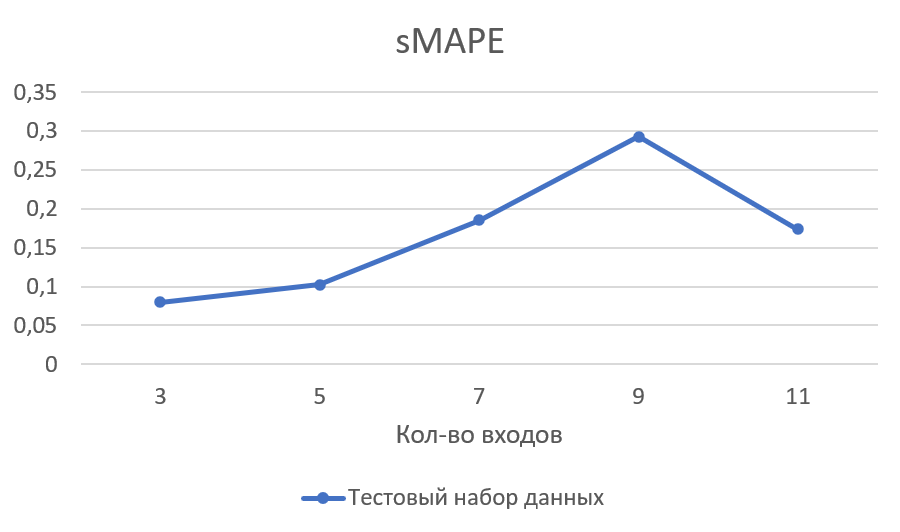
\includegraphics[scale=0.7]{mackey-glass-inference-smape}
	\caption{График значений метрики sMAPE на обучающем и тестовом наборах данных при различных размерах окна запаздывания, количестве правил --- 30.}
	\label{fig:mackey-glass-inference-smape}
\end{figure}

По итогу проведенного эксперимента лучший показатель качества прогнозирования по этой метрике на рисунке \cref{fig:mackey-glass-inference-smape} достигается при размере окна запаздывания --- 3 точки. 

%
Достигнутое в этом случае значение $sMAPE = 8\%$ при количестве правил 30, заметно превосходит точность моделирования незашумленной последовательности Mackey-Glass (M-G) с использованием синглтонной фаззификации со значением $sMAPE \approx 40\%$ в \cite{Pekaslan2020}. Также полученное качество прогнозирования сопоставимо со значением этой метрики при аналогичной конфигурации эксперимента прогнозирования временного ряда M-G в той же публикации, где для достижения точности моделирования временной последовательности $sMAPE \approx 10\%$ используется нечеткая система типа Мамдани, содержащая 184 правила\footnote{Непосредственно в самой статье не указано количество используемых правил. Однако авторами этой статьи опубликован программный код описанного в статье метода, запустив который удалось воспроизвести проводимые авторами эксперименты и восстановить количество правил в их нечетких системах.} в базе правил для не зашумленного временного ряда M-G и 597, 402, 312 правил для различных конфигураций и амплитуды добавленного шума. Данные наблюдения показывают, что \textbf{метод регрессии временных рядов на основе логического нечеткого вывода при несинглтонной фаззификации значительно превосходит качество регрессии с использованием синглтонной фаззификации, а также имеет сопоставимую с методом регрессии Мамдани при несинглтонной фаззификации точность, но при меньшем количестве правил} за счет возможности построения более сложной функции аппроксимации.

Второй эксперимент посвящен применению разработанного метода для прогнозирования помесячного объема транзакций безналичных платежей корпоративным клиентам банка. Источником неопределенности в этом наборе данных является стохастический характер динамики временной последовательности. Поэтому в этом эксперименте также использовалась процедура адаптивной несинглтонной фаззификации. В качестве метрики использовалась RMAE (relative MAE) --- отношение средней абсолютной ошибки к математическому ожиданию средних по рядам клиентов:
\[
RMAE = \frac{MAE}{\mathbb{E}[\mathbb{E}[s_t]]}.
\]

По итогу эксперимента было получено значение метрики $RMAE = 0.112/0.147$ при прогнозировании на один/три месяца соответственно. Это превосходит на $12\%/5\%$ качество прогнозирования с использованием многослойного перцептрона со значениями $RMAE = 0.128/0.157$. 




%В заключении перечислены основные научные результаты, каждый из которых подтверждён приведёнными формулами, схемами, экспериментальными графиками и таблицами: (1) формализация и аналитическая реализация метода на основе НЗИ; (2) снижение вычислительной сложности и эффективная параллельная реализация; (3) экспериментальная оценка на реальных задачах; (4) создание программной системы с поддержкой GPU и интеграцией в Python.

В \textbf{заключении} сделаны выводы о полученных в процессе работы результаты.

\pdfbookmark{Заключение}{conclusion}                                  % Закладка pdf
\section*{Заключение}
В результате выполнения работы удалось выработать метод нечеткого вывода на основе нечеткого значения истинности, позволяющий использовать тип фаззификации non-singleton при полиномиальной сложности вывода от количества входов, а также показано улучшение качества прогнозирования временных рядов с использованием логического типа вывода в сравнении с синглтонной фаззификацией и выводом типа Мамдани. В работе решены поставленные задачи и получены следующие результаты:
%% Согласно ГОСТ Р 7.0.11-2011:
%% 5.3.3 В заключении диссертации излагают итоги выполненного исследования, рекомендации, перспективы дальнейшей разработки темы.
%% 9.2.3 В заключении автореферата диссертации излагают итоги данного исследования, рекомендации и перспективы дальнейшей разработки темы.
\begin{enumerate}
  \item Анализ состояния исследований в области анализа качественных/за­шумленных данных с использованием нечеткого моделирования показал недостатки существующих методов. В частности, было выявлено отсут­ствие таких методов для моделирования систем и процессов, имеющих множество качественных/зашумленных входов, которые работали бы с полиномиальной вычислительной сложностью от количества входов и не были бы связаны со значительными упрощениями теории нечеткого логического вывода.
  \item Для логического подходов были разработаны методы, позволяющие осуществлять нечеткий логиеский вывод с полиномиаль­
  ной сложностью для произвольного набора используемых t-норм, что обеспечивает более гибкую настройку таких систем. Для определенных частных случаев в наборах используемых норм были разработаны опти­мизированные версии этих методов с использованием меры возможности.
  \item Разработан метод классификации для объектов со многими нечеткими входах\ldots
  \item Математическое моделирование показало \ldots
  \item Для выполнения поставленных задач был создан \ldots
\end{enumerate}


\pdfbookmark{Литература}{bibliography}                                % Закладка pdf
%При использовании пакета \verb!biblatex! список публикаций автора по теме
%диссертации формируется в разделе <<\publications>>\ файла
%\verb!common/characteristic.tex!  при помощи команды \verb!\nocite!

\ifdefmacro{\microtypesetup}{\microtypesetup{protrusion=false}}{} % не рекомендуется применять пакет микротипографики к автоматически генерируемому списку литературы
\urlstyle{rm}                               % ссылки URL обычным шрифтом
\ifnumequal{\value{bibliosel}}{0}{% Встроенная реализация с загрузкой файла через движок bibtex8
	\renewcommand{\bibname}{\large \bibtitleauthor}
	\nocite{*}
	\insertbiblioauthor           % Подключаем Bib-базы
	%\insertbiblioexternal   % !!! bibtex не умеет работать с несколькими библиографиями !!!
}{% Реализация пакетом biblatex через движок biber
	% Цитирования.
	%  * Порядок перечисления определяет порядок в библиографии (только внутри подраздела, если `\insertbiblioauthorgrouped`).
	%  * Если не соблюдать порядок "как для \printbibliography", нумерация в `\insertbiblioauthor` будет кривой.
	%  * Если цитировать каждый источник отдельной командой --- найти некоторые ошибки будет проще.
	%
	
	
	\ifnumgreater{\value{usefootcite}}{0}{
		\begin{refcontext}[labelprefix={}]
			\ifnum \value{bibgrouped}>0
			\insertbiblioauthorgrouped    % Вывод всех работ автора, сгруппированных по источникам
			\else
			\insertbiblioauthor      % Вывод всех работ автора
			\fi
		\end{refcontext}
	}{
		\ifnum \totvalue{citeexternal}>0
		\begin{refcontext}[labelprefix=A]
			\ifnum \value{bibgrouped}>0
			\insertbiblioauthorgrouped    % Вывод всех работ автора, сгруппированных по источникам
			\else
			\insertbiblioauthor      % Вывод всех работ автора
			\fi
		\end{refcontext}
		\else
		\ifnum \value{bibgrouped}>0
		\insertbiblioauthorgrouped    % Вывод всех работ автора, сгруппированных по источникам
		\else
		\insertbiblioauthor      % Вывод всех работ автора
		\fi
		\fi
		%  \insertbiblioauthorimportant  % Вывод наиболее значимых работ автора (определяется в файле characteristic во второй section)
		\begin{refcontext}[labelprefix={}]
			\insertbiblioexternal            % Вывод списка литературы, на которую ссылались в тексте автореферата
		\end{refcontext}
		% Невидимый библиографический список для подсчёта количества внешних публикаций
		% Используется, чтобы убрать приставку "А" у работ автора, если в автореферате нет
		% цитирований внешних источников.
		\printbibliography[heading=nobibheading, section=0, env=countexternal, keyword=biblioexternal, resetnumbers=true]%
	}
	\clearpage
}
\ifdefmacro{\microtypesetup}{\microtypesetup{protrusion=true}}{}
\urlstyle{tt}                               % возвращаем установки шрифта ссылок URL
      % Содержание автореферата

%%% Выходные сведения типографии
\newpage\thispagestyle{empty}

\vspace*{0pt plus1fill}

\small
\begin{center}
    \textit{\thesisAuthor}
    \par\medskip

    \thesisTitle
    \par\medskip

    Автореф. дис. на соискание ученой степени \thesisDegreeShort
    \par\bigskip

    Подписано в печать \blank[\widthof{999}].\blank[\widthof{999}].\blank[\widthof{99999}].
    Заказ № \blank[\widthof{999999999999}]

    Формат 60\(\times\)90/16. Усл. печ. л. 1. Тираж 100 экз.
    %Это не совсем формат А5, но наиболее близкий, подробнее: http://ru.wikipedia.org/w/index.php?oldid=78976454

    Типография \blank[0.5\linewidth]
\end{center}
\cleardoublepage

\end{document}
